%************************************************
\chapter{Redes long short-term memory para resolver la ecuación de Schrödinger}\label{ch:LSTMapplied}
% ************************************************
\section{Introducción}
En el capítulo anterior se desarrollaron conceptos básicos generales de las redes neuronales, actualmente existen diversos tipos de redes que se aplican a problemas comunes y que se distinguen por su arquitectura.
\\
En este capítulo se abordará un modelo particular de red llamado \emph{long short-term memory} (\acs{LSTM}), que pertenece a un tipo de redes llamadas \emph{redes neuronales recurrentes} (\acs{RNN}, por sus siglas en inglés). Este tipo de redes es comúnmente utilizada cuando los atributos en el conjunto de datos están relacionados entre sí, o guardan una dependencia.
\\\\
En la sección \autoref{sec:lstm} se desarrollará la arquitectura de las redes \acs{LSTM}, así como sus aplicaciones más comunes, haciendo énfasis a las series de tiempo, que son de particular interés en el presente trabajo, pues la evolución temporal de un paquete de onda puede tratarse como un problema de series de tiempo, encontrando así una manera de abordar el problema de propagar una onda en el tiempo utilizando una red \acs{LSTM}.
\\
En la sección \autoref{sec:Project} se implementa el modelo de \acs{LSTM} que servirá como propagador $\mathcal{U}$ en la ecuación de Schrödinger Dependiente del Tiempo (\autoref{eq:TDSE ket}) para los potenciales $V(r,t)$ revisados en la sección \autoref{sec:ProtonTransfer}.
\\
A lo largo de la sección se presentará el conjunto de datos de entrenamiento de la red, así como los parámetros del modelo del potencial que se utilizaron para su obtención; también se presentarán los hiper-parámetros empleados en la red. Finalmente, en la sección \autoref{sec:Resultados} se presentan los resultados y predicciones obtenidas con del modelo.

\section{Redes neuronales recurrentes}\label{sec:RNN}
Como se mencionó anteriormente, las \acs{RNN}s se emplean cuando entre los atributos del conjunto de datos existen relaciones. Un dato de entrada para este tipo de redes puede verse de la siguiente forma:

\begin{equation}
  \label{eq:xdataRNN}
  \vec{X} = (\vec{x}_0, \vec{x}_1, \dots , \vec{x}_n)
\end{equation}

en donde cada $\vec{x}_t$ es un vector de dimensión $d$ recibido al tiempo $t$. Para cada tiempo $t$ se tiene un valor de salida: $\vec{y}_t$ con la misma dimensión.
\\
Algunos ejemplos de aplicaciones se muestran a continuación:

\begin{itemize}[label=\textcolor{CTtitle}{\textbullet}]
\item \emph{Secuencias de texto:} En donde la importancia o información de una palabra depende del contexto en el que se encuentra dentro de una oración. Cada palabra\footnote{En este caso, la dimensión $d$ hace referencia al número de palabras que tiene el léxico utilizado.}: $\vec{x}_t$,  puede verse como un atributo relacionado a la palabra anterior en una oración: $\vec{x}_{t-1}$, o a la palabra siguiente: $\vec{x}_{t+1}$.
 \item \emph{Series de tiempo:} $\vec{x}_t$ en este caso puede almacenar $d$ valores, que pueden ser, por ejemplo, los correspondientes al valor de una función $f(x,t)$ en una maya de $d$ puntos en el espacio $x$ al tiempo $t$. En este tipo de configuración la salida $\vec{y}_t$ podría ser la predicción pronosticada de $\vec{x}_{t+1}$.
 \end{itemize}
  
Un diagrama sencillo de una \acs{RNN} se muestra en la \autoref{fig:RNN}, en donde un auto-bucle actualizará el \textbf{estado oculto} $\vec{h}_t$ a cada tiempo $t$ después de la entrada $\vec{x}_t$:
\begin{equation}
  \label{eq:hidden}
  \vec{h}_t = Tanh(W_{xh}\vec{x}_t + W_{hh} \vec{h}_{t-1})
\end{equation}
%\begin{equation}
%  \vec{h}_t = f(\vec{h}_{t-1}, \vec{x}_t)
%\end{equation}
donde \emph{Tanh} es la función de activación, que está siendo aplicada a cada elemento del vector resultante de la multiplicación y suma de las matrices de peso $W$ por los vectores $\vec{x}_t$ y $\vec{h}_{t-1}$ para cada tiempo $t$. La salida, por su parte, está dada por:
\begin{equation}
  \vec{y}_t = W_{hy}\vec{h}_t
\end{equation}

\begin{figure}[!htbp]
  \centering
  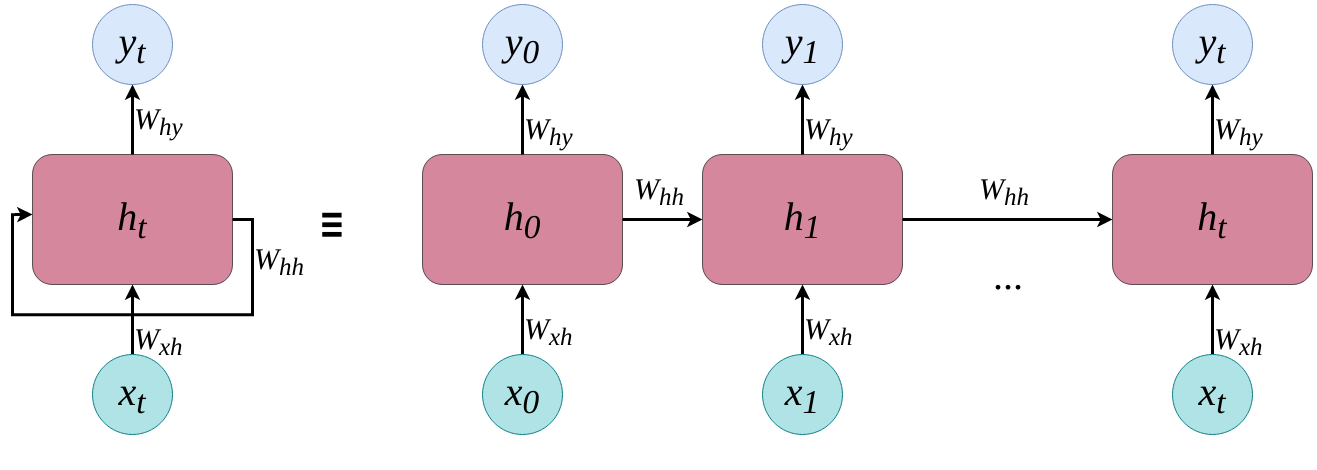
\includegraphics[width=0.9\textwidth]{./img/RNN.png}
  \caption{Diagrama de una \acs{RNN} y su representación en capas de tiempo.}
  \label{fig:RNN}
\end{figure}

En la \autoref{fig:RNN}, a la derecha se muestra la representación de la \acs{RNN} en capas para cada tiempo, en donde es importante notar que las matrices de peso $W$ son las mismas en cada tiempo $t$, de manera que ecuación de recurrencia \autoref{eq:hidden} aplica la misma función.
\\

Uno de los principales problemas de las \acs{RNN}s en la práctica es en el entrenamiento, pues el gradiente tiende a desvanecerse o incrementar excesivamente, debido a la inestabilidad que produce la multiplicación de forma recursiva de las matrices de peso $W$, problema que puede incrementarse cuanto más grande sea la secuencia de tiempo que procesa la red y cuantas más capas ocultas tenga. \cite{Nielsen:2018}
\\
Una alternativa que previene este problema es el cambio de la relación de recurrencia para el estado oculto $\vec{h}_t$ (\autoref{eq:hidden}) mediante el uso de la \emph{memoria a largo plazo} de una red \acs{LSTM}, que se abordará en la siguiente sección.

\section{Redes long short-term memory}\label{sec:lstm}

Las \textbf{redes long short-term memory} son un tipo de \acs{RNN} diseñadas para mitigar los problemas con el gradiente que estas tienen en el entrenamiento. La manera en la que realizan esto es cambiando las condiciones de recurrencia de cómo el estado oculto $\vec{h}_t$ es propagado en el tiempo, para ello, se introduce un nuevo vector llamado \textbf{celda de estado} o \textbf{cell state} en inglés denotado por $\vec{c}_{t}$ de la misma dimensión de $\vec{h}_t$, que puede interpretarse como una \emph{memoria a largo plazo} que retiene parte de la información de las celdas de estados de tiempos pasados. \cite{Nielsen:2018}

\begin{figure}[!htbp]
  \centering
  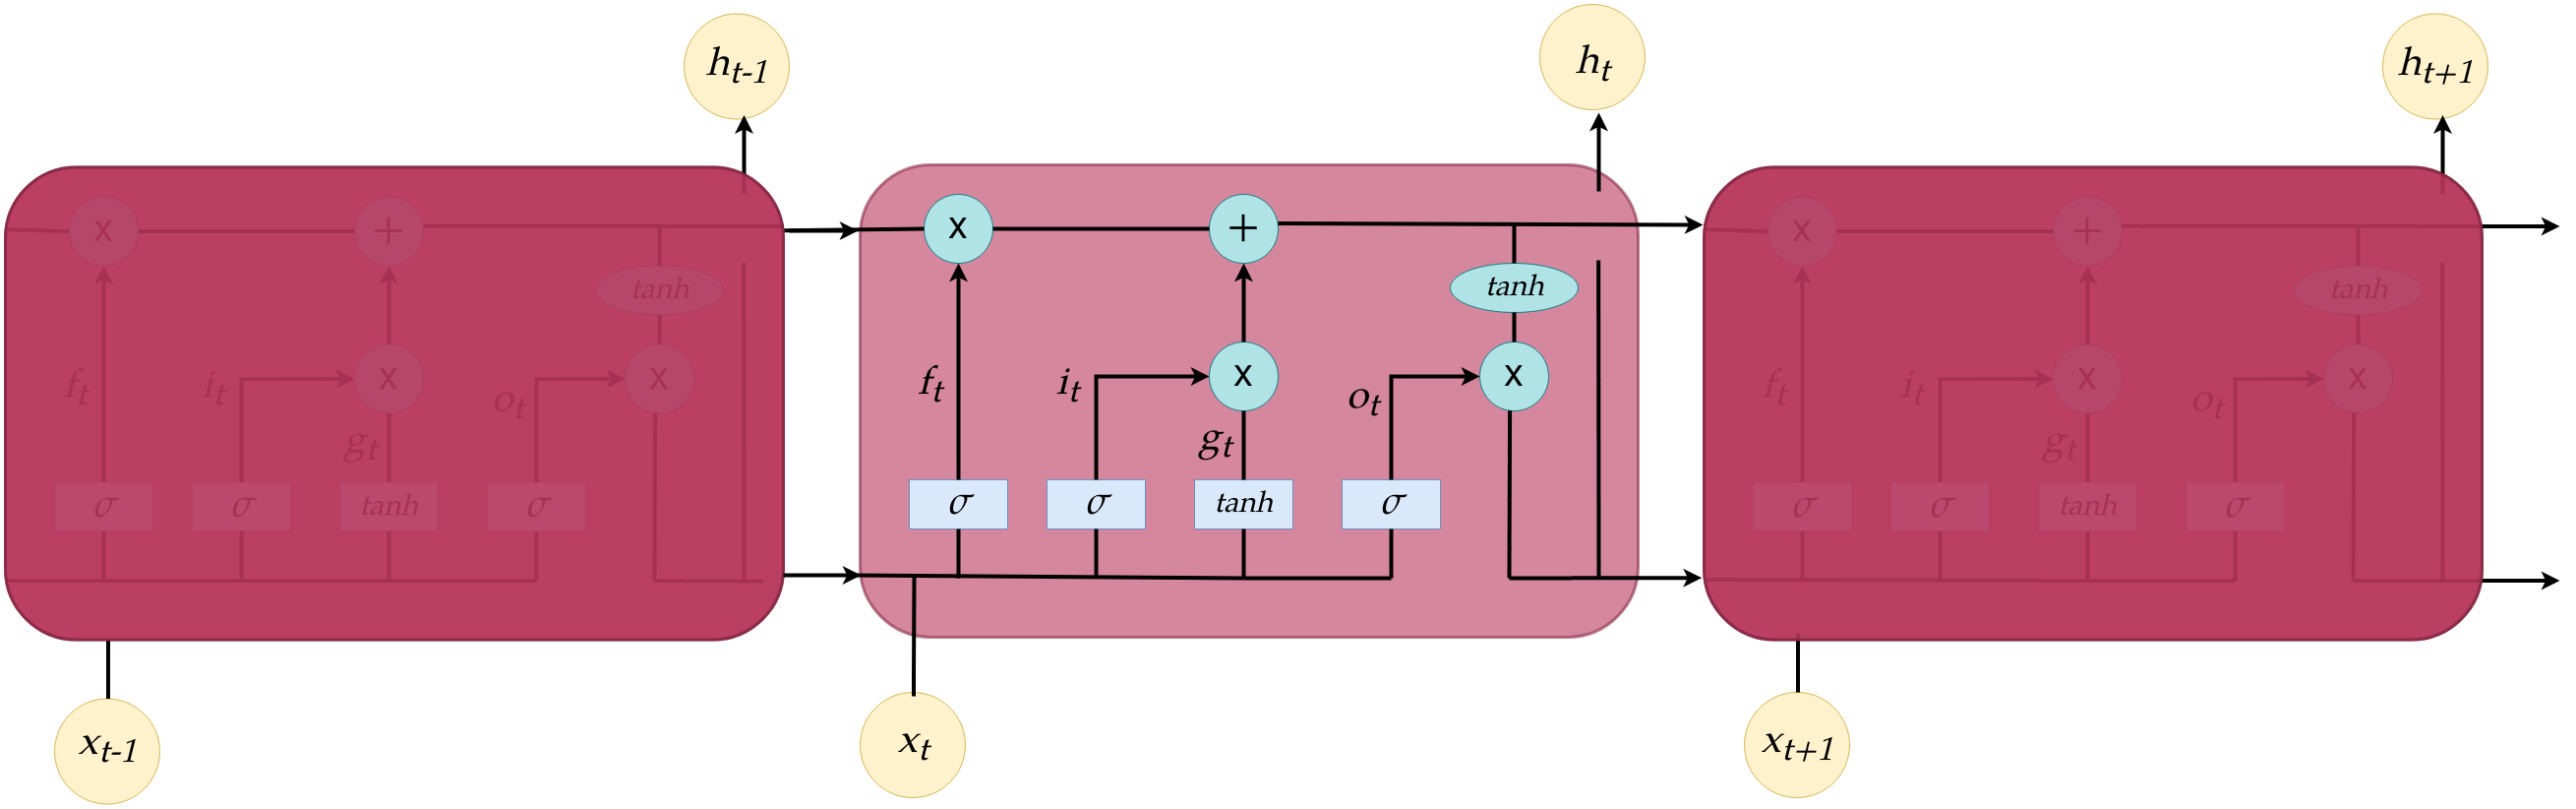
\includegraphics[width=0.9\textwidth]{./img/LSTM_layerS.drawio.png}
  \caption{Diagrama de una \acs{LSTM} representada en capas de tiempo.}
  \label{fig:LSTMlayerS}
\end{figure}

El diagrama de la \autoref{fig:LSTMlayerS} muestra la estructura de una \acs{LSTM} desplegada en capas de tiempo, su forma en cadena es igual a la de las \acs{RNN}s mencionadas en la sección anterior, sin embargo, cada bloque de memoria (recuadros rosas) tiene una arquitectura particular más compleja que la de una \acs{RNN} común.

\subsection{Arquitectura}\label{sec:LSTM_Arch}
La \autoref{fig:LSTMlayer} muestra un bloque de memoria de una \acs{LSTM}, en donde se observa cómo interactúan los vectores de estado oculto y de celda de estado pasados: $\vec{h}_{t-1}$ y $\vec{c}_{t-1}$ con funciones llamadas compuertas o gates en inglés, denotadas por $\vec{f}_t$, $\vec{i}_t$, $\vec{o}_t$ y operaciones básicas como suma y multiplicación, para producir nuevos vectores $\vec{h}_{t}$ y $\vec{c}_{t}$. Al tiempo $t=0$, los vectores de estado oculto y de celda de estado comienzan inicializados con un valor aleatorio. \cite{Olah}

\begin{figure}[!htbp]
  \centering
  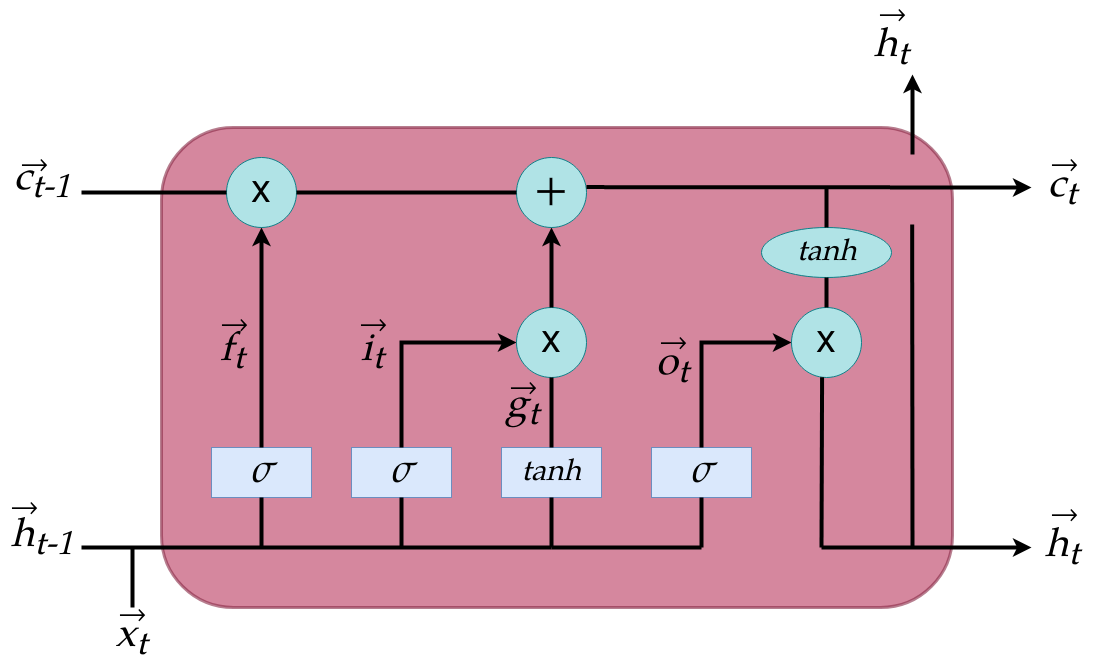
\includegraphics[width=0.7\textwidth]{./img/LSTM_layer.png}
  \caption{Diagrama de un bloque de memoria de una \acs{LSTM}.}
  \label{fig:LSTMlayer}
\end{figure}

Una compuerta llamada \textbf{forget} $\vec{f}$, decide qué información proveniente del tiempo anterior $t-1$ se mantiene y cual no, tomando en consideración también la entrada $\vec{x}_t$, aplicando la función sigma (es decir, $\vec{f}$ es una capa \emph{Sigmoid}):

\begin{equation}\label{eq:ft}
\vec{f}_t = \sigma(W_{xf}\vec{x}_t + W_{hf}\vec{h}_{t-1} + b_f)
\end{equation}

En donde $W$ y $b$ con sus correspondientes subíndices representan las matrices de peso y vectores de sesgo correspondientes a cada capa oculta. \\
Posteriormente, para decidir qué nueva información será incluida a la celda de estado se calculan:

\begin{equation}\label{eq:it}
\vec{i}_t = \sigma(W_{xi}\vec{x}_t + W_{hi}\vec{h}_{t-1} + b_i)
\end{equation}
\begin{equation}
  \label{eq:gt}
\vec{g}_t = Tanh(W_{xg}\vec{x}_t + W_{hg}\vec{h}_{t-1} + b_g)  
\end{equation}

en donde $\vec{i}$ es una capa \emph{Sigmoid}, llamada compuerta \textbf{input}, y $\vec{g}$ es una capa \emph{Tanh} que genera un vector con valores nuevos que son candidatos para ser agregados a la nueva celda de estado $\vec{c}_t$.
\\
La actualización de la celda de estado se da como:

\begin{equation}\label{eq:ct}
\vec{c}_t = \vec{f}_t \ast \vec{c}_{t-1} + \vec{i}_t \ast \vec{g}_t
\end{equation}

en donde $\ast$ representa el \emph{producto Hadamard}, en donde la multiplicación de los vectores se realiza elemento por elemento. Finalmente, la salida esta dada por:

\begin{equation}\label{eq:ot}
\vec{o}_t = \sigma(W_{xo}\vec{x}_t + W_{ho}\vec{h}_{t-1} + b_o)
\end{equation}

\begin{equation}\label{eq:ht}
\vec{h}_t = \vec{o}_t\ast Tanh(\vec{c}_t)
\end{equation}

en donde $\vec{o}$ es una capa \emph{Sigmoid} llamada compuerta \textbf{output}, y el vector $\vec{h}_t$ es el estado oculto al tiempo $t$, que servirá como entrada, junto con el vector de celda de estado $\vec{c}_t$ para el bloque de memoria del tiempo $t+1$, como se muestra en la \autoref{fig:LSTMlayerS}.

% ************************************************************
% ************************************************************
% PROYECTO
% ************************************************************
% ************************************************************

\section{Propagación temporal de funciones de onda con LSTM}\label{sec:Project}

En esta sección se implementa una red \acs{LSTM} para predecir la evolución en un periodo de tiempo largo\footnote{Respecto a la escala de tiempo característico del sistema físico estudiado.} de un paquete de onda a un tiempo inicial $\psi(r,t)$ bajo un potencial dependiente del tiempo $V(r,t)$ en intervalos de tiempo$\Delta t$. Se utilizó como referencia un trabajo previo \cite{Main:2021} en donde se implementó un modelo de perceptrón multicapa para obtener el paquete de onda propagado un paso de tiempo $\Delta t$.

\subsection{Obtención de datos}\label{sec:6.4.1}

El conjunto de datos de entrenamiento utilizado se obtuvo generando 8000 trayectorias de $200\,fs$, cada una con un $\Delta t = 1\,fs$. El diagrama de la \autoref{fig:DiagTraj} muestra una trayectoria, en donde $\psi(r,t_l)r$ con $l=0,\dots 200$ representa la parte real del paquete de onda, $\psi(r,t_l)i$ la parte imaginaria y $V(r,t_l)$ el potencial.

\begin{figure}[H]
  \centering
  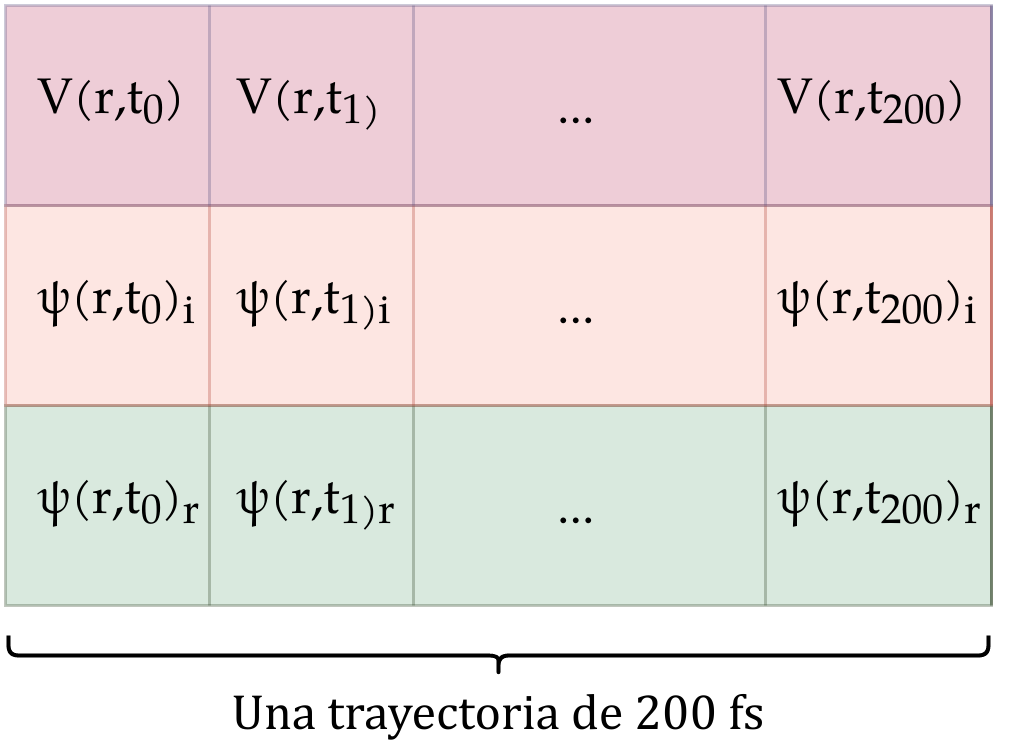
\includegraphics[width=0.7\textwidth]{./img/DiagTrayectoria.png}
  \caption{Diagrama de una trayectoria generada.\\Para cada tiempo $t_i$ la onda $\psi(r,t_i)$ contiene el valor de la onda en los $N=32$ puntos en la malla del espacio de posiciones en $r$.}
  \label{fig:DiagTraj}
\end{figure}

Para cada trayectoria, los paquetes de onda iniciales, es decir al tiempo $t=0$, se definieron como ondas Gaussianas: (\autoref{fig:Gauss})
\begin{figure}[H]
  \centering
  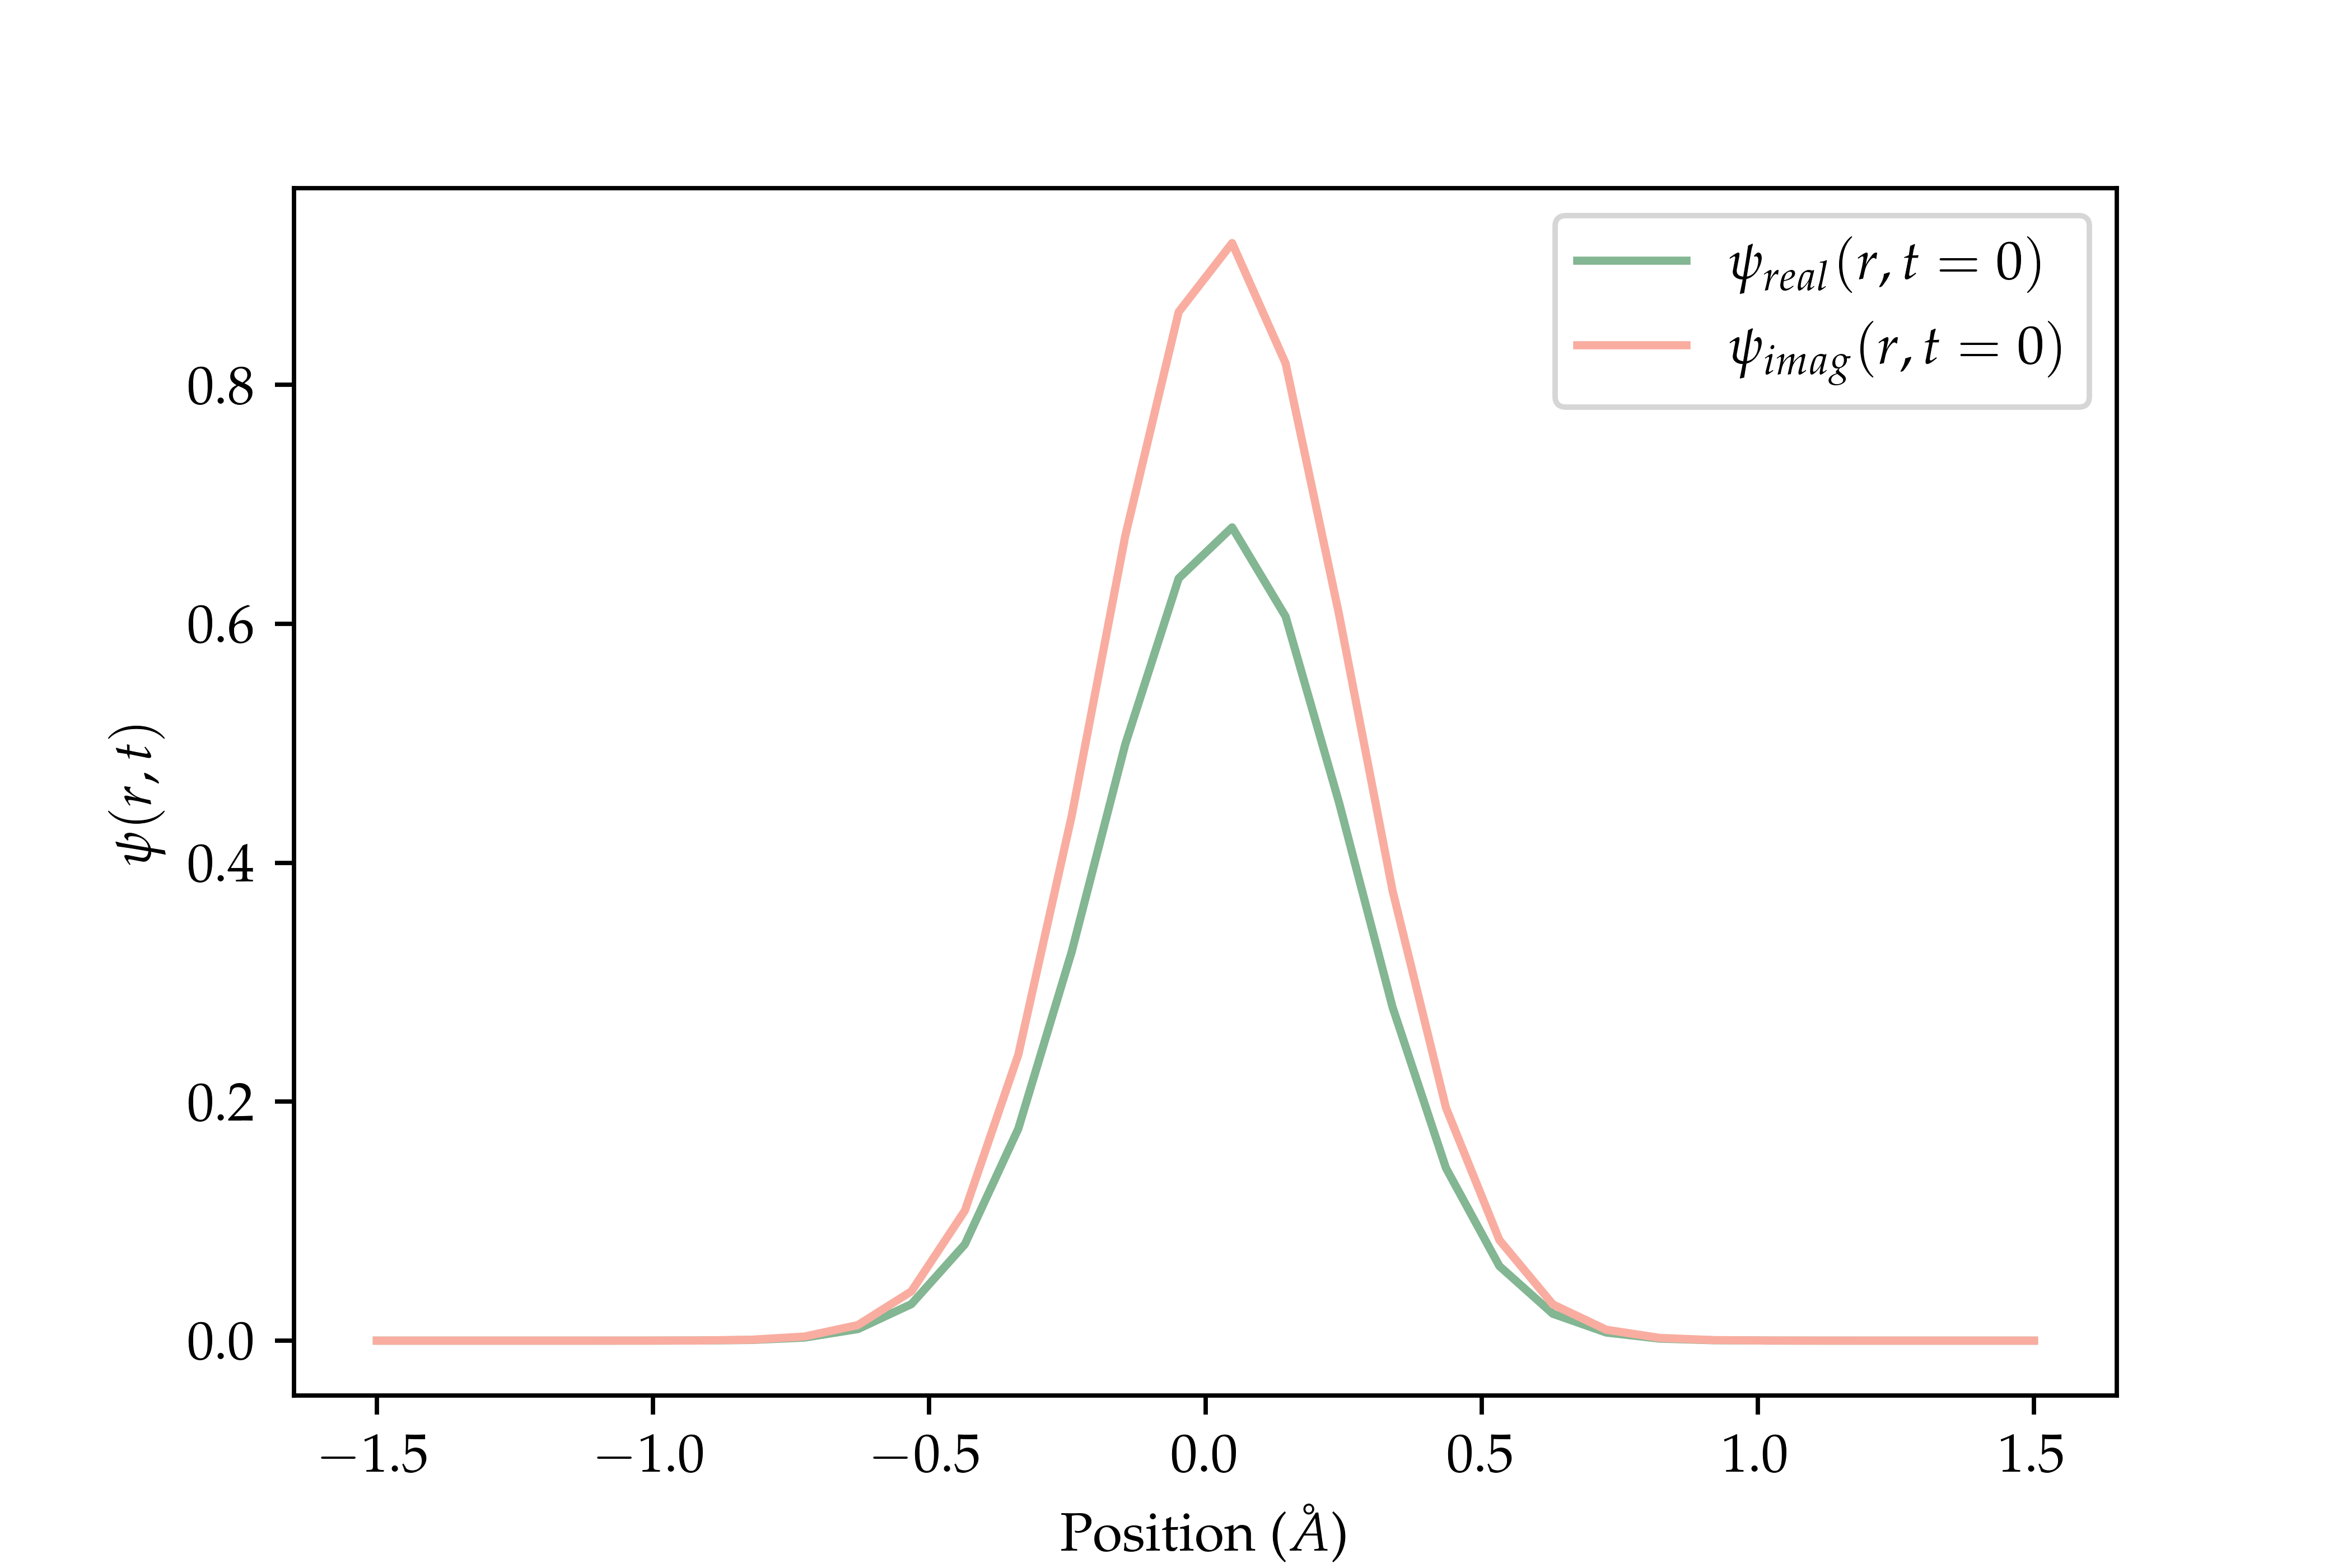
\includegraphics[width=1\textwidth]{./img/DataWave.png}
  \caption{Parte real y compleja de un paquete de onda inicial $\psi(r,t=0)$.}
  \label{fig:Gauss}
\end{figure}

\begin{equation}
  \label{eq:gaussian}
  \psi(r,0) = C_i\cdot \frac{1}{\sigma\sqrt{2\pi}}\exp{\frac{-(r-\mu)^2}{2\sigma^2}}
\end{equation}
en donde $\mu$ y $\sigma$ son valores aleatorios elegidos de una distribución uniforme de $(-0.5,0.5)\mathring{A}$ y $(0.1,0.3)\mathring{A}$ respectivamente. $C_i$ es un número complejo aleatorio elegido de tal manera que la onda esté normalizada, es decir:
$$\bra{\psi(r,0)}\ket{\psi(r,0)} = 1$$

Para propagar la onda se utilizó el método \acs{DVR} revisado en la sección \autoref{sec:DVRapp} con una malla de $N=32$ puntos, con $a=r_0=-1.5\mathring{A}$ y $b=r_{N-1}=1.5\mathring{A}$ (\autoref{eq:malla}).
\\
El modelo de potencial $V(r,t)$ utilizado fue el mismo que se usó en la sección \autoref{sec:ProtonTransfer}. Para cada trayectoria se eligieron valores de parámetros para el modelo de potencial aleatorios entre rangos especificados en la \autoref{tab:RangeValuesPot}. En la \autoref{fig:Pote} se muestra un ejemplo de un potencial generado.
\begin{figure}[H]
  \centering
  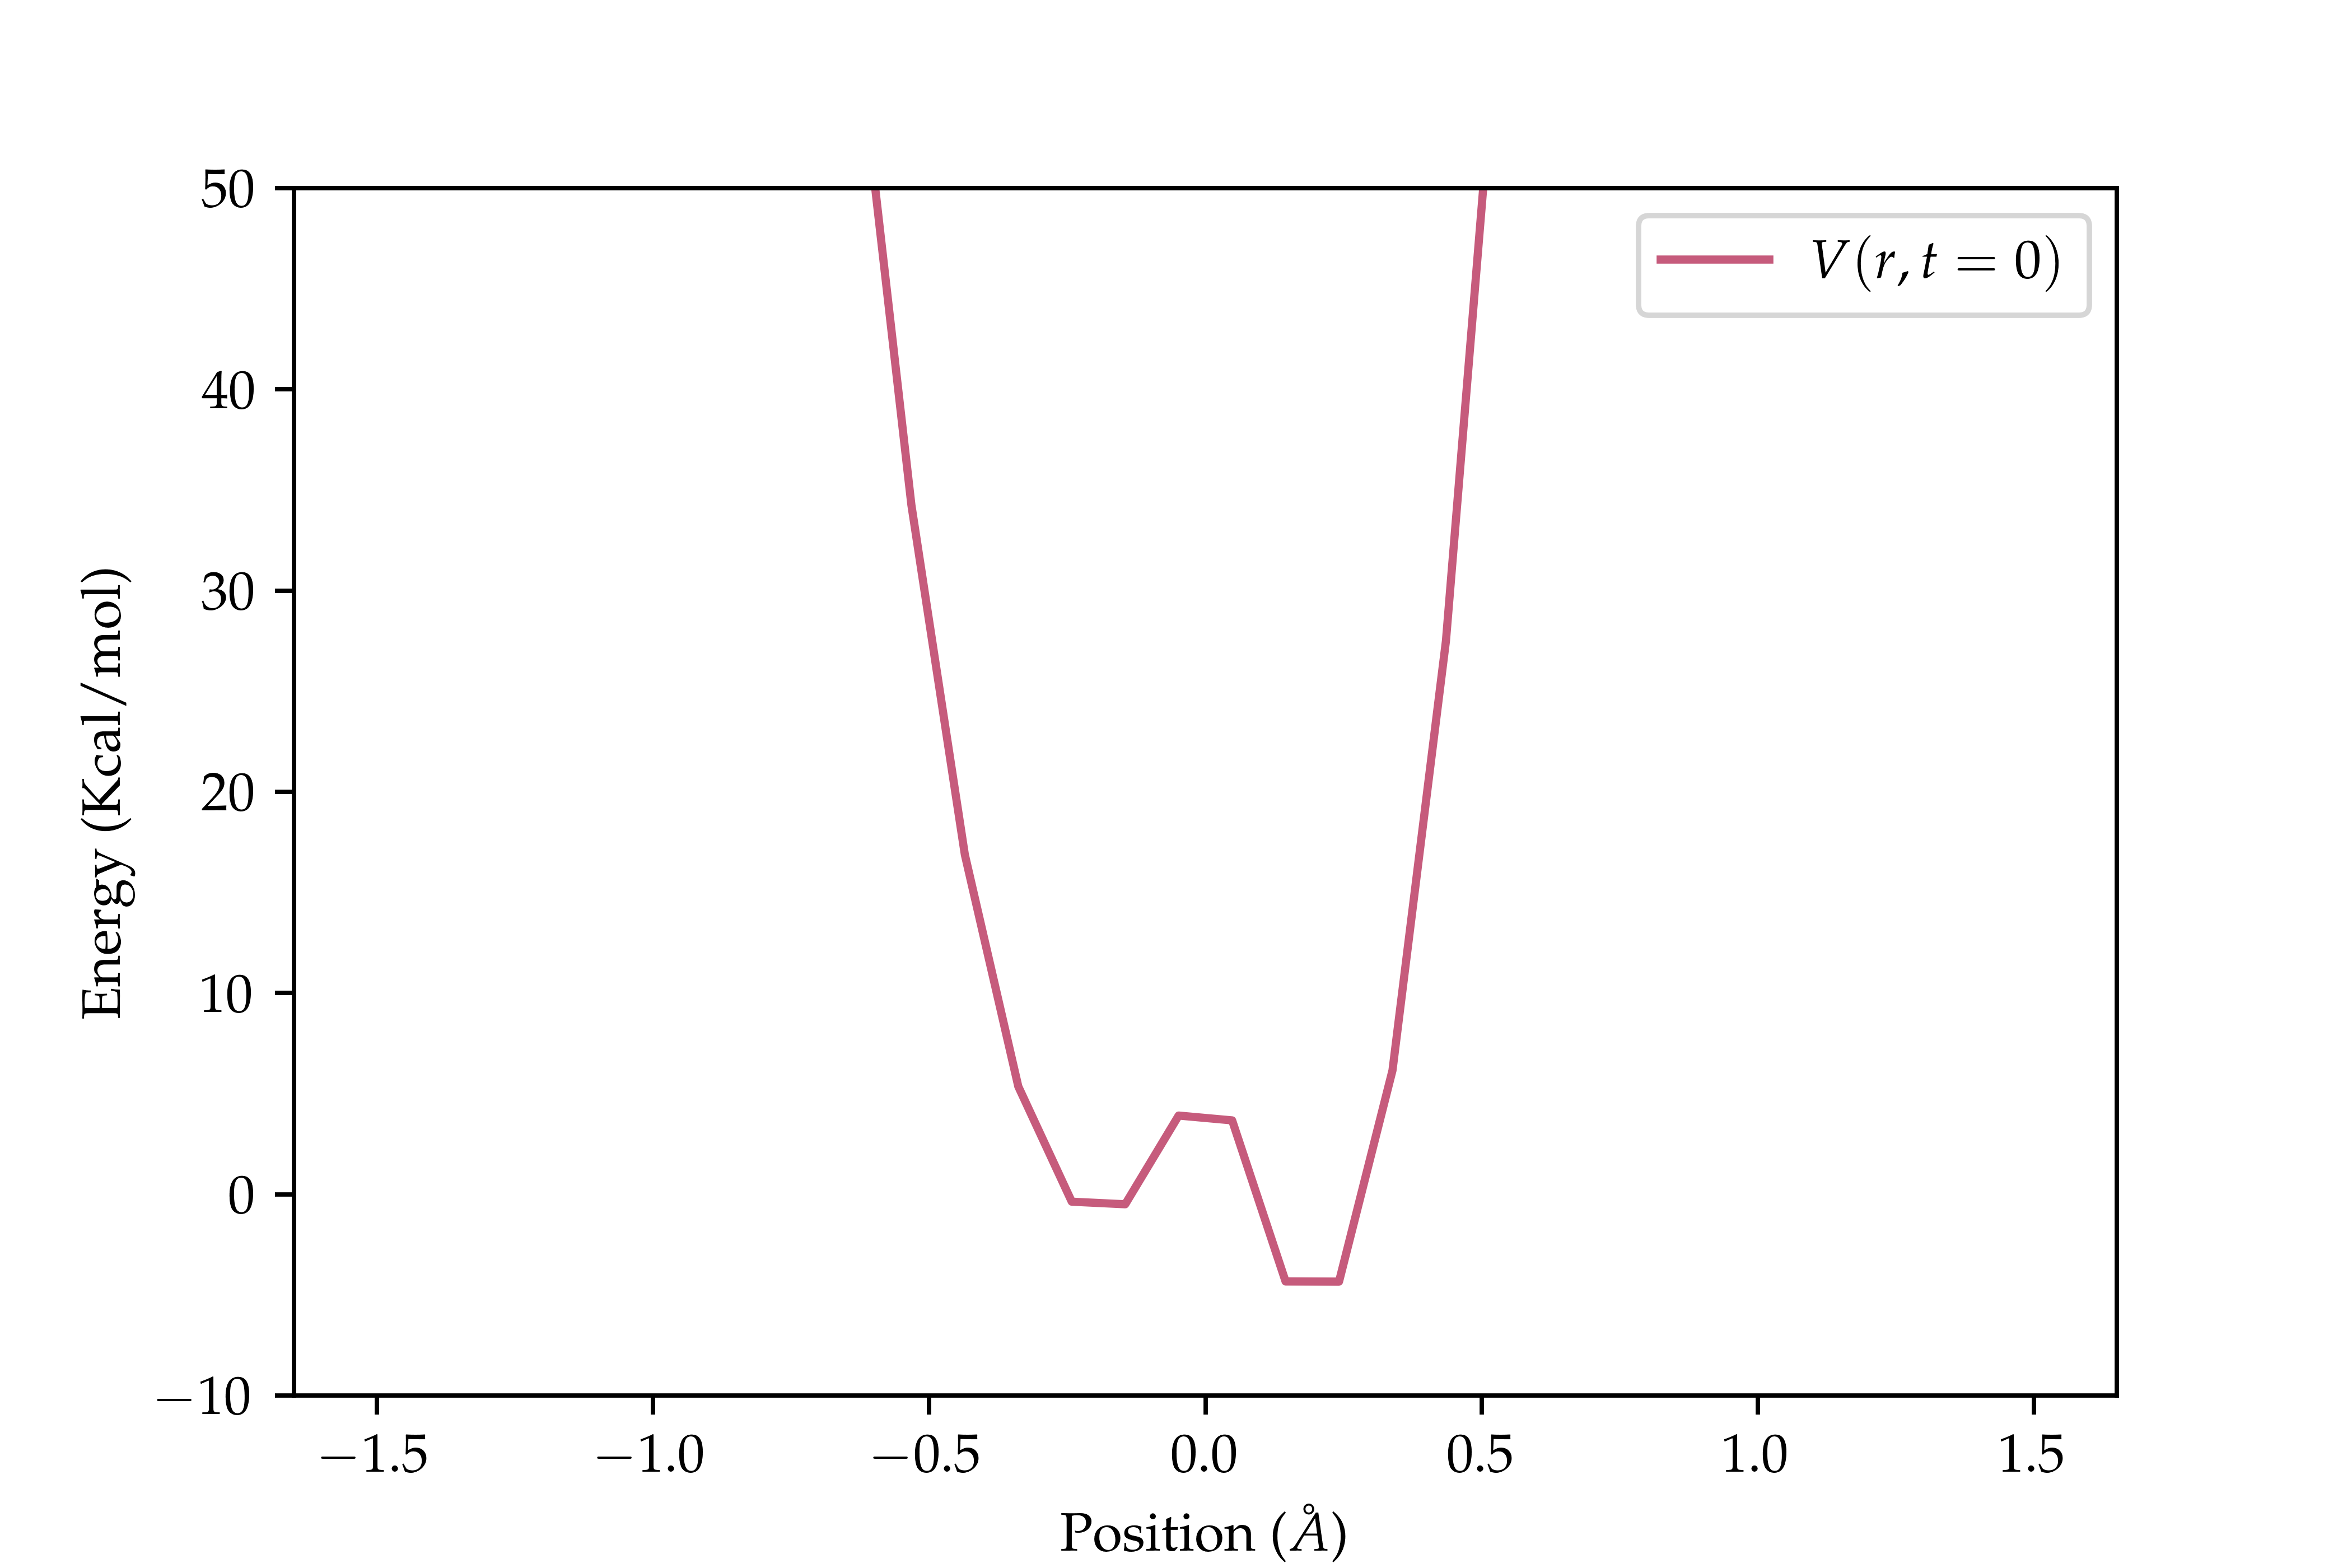
\includegraphics[width=1\textwidth]{./img/DataPot.png}
  \caption{Potencial inicial al tiempo $t=0$}
  \label{fig:Pote}
\end{figure}

En el repositorio \href{https://github.com/Jessi-MM/PropagatorLearning/tree/main/Data_Gaussian}{\faGithub Trayectorias} se encuentran los datos generados\footnote{\textcolor{CTtitle}{\faExclamationTriangle} Para trabajos futuros, se recomienda fuertemente NO crear un directorio por dato, pues esto generó problemas de peso y tiempo de cómputo. Un solo archivo con extensión .csv o .hdf5 es más recomendado para guardar una mayor cantidad de datos.}. Cada carpeta contiene los directorios y archivos siguientes:

 \begin{forest}
      for tree={
        font=\ttfamily,
        grow'=0,
        math content,
        align=center,
        child anchor=west,
        parent anchor=south,
        anchor=west,
        calign=first,
        inner xsep=7pt,
        edge path={
          \noexpand\path [draw, \forestoption{edge}]
          (!u.south west) +(7.5pt,0) |- (.child anchor) pic {folder} \forestoption{edge label};
        },
        % style for your file node 
        file/.style={edge path={\noexpand\path [draw, \forestoption{edge}]
          (!u.south west) +(7.5pt,0) |- (.child anchor) \forestoption{edge label};},
          inner xsep=2pt,font=\small\ttfamily
                     },
        before typesetting nodes={
          if n=1
            {insert before={[,phantom]}}
            {}
        },
        fit=band,
        before computing xy={l=15pt},
      }  
    [Trayectorias
      [data0
      [Potential
      [0-Potential.npy\\$\vdots$,file]
      [200-Potential.npy,file
      ]
        ]
        [Wavepacket
        [0-Wavepacket.npy\\$\vdots$,file
        ]
        [200-Wavepacket.npy,file
        ]
        ]
      ]
    ]
 \end{forest}

 En donde \texttt{data0} corresponde a la trayectoria $0$. El archivo \emph{0-Potential.npy} es un arreglo de $N=32$ entradas que corresponde al valor del potencial al tiempo $t=0\,fs$, el archivo \emph{0-Wavepacket.npy} es un arreglo de $N=32$ entradas complejas que corresponden al paquete de onda al tiempo $t=0\,fs$; así respectivamente para cada tiempo hasta $t=200\,fs$. Además de los datos, se encuentra un archivo de texto: \emph{ValuesPotential.txt}, en donde se registran los valores de los parámetros para generar el potencial, es decir, los valores exactos elegidos de la \autoref{tab:RangeValuesPot}.
 \\
 
 El código para generar las trayectorias se encuentra en el repositorio: \href{https://github.com/Jessi-MM/PropagatorLearning/blob/main/src/Proton_Transfer_DataGenerate.ipynb}{\faGithub Generación de datos}, que contiene dos clases: \emph{Potential\_System}, que contiene las ecuaciones del modelo del potencial y la clase \emph{ProtonTransfer}, con la que se generan las trayectorias. A continuación se muestra un ejemplo para generar una trayectoria, con la información que muestra el diagrama de la \autoref{fig:DiagTraj}:

 \begin{lstlisting}[language=Python, morekeywords={ProtonTransfer, True, False}]
   trayectoria0 = ProtonTransfer(n=32, a=-1.5, b=1.5, time=True, var_random=True, save_dir='data0')
   trayectoria0.vector_potential(t=200,step=1)
   trayectoria0.evolution_wp(t=200, step=1, gaussiana=True)\end{lstlisting}

En donde se utilizan las siguientes variables:
\begin{itemize}[label=\textcolor{CTtitle}{\textbullet}]
\item n: Número de puntos en la malla
\item a: Punto inicial de la malla $[\mathring{A}]$
\item b: Punto final de la malla $[\mathring{A}]$
\item time: True o False. Determina si se utiliza un potencial dependiente del tiempo: True, o independiente del tiempo: False  
\item var\_random: True o False. True inicia las variables de manera aleatoria para el potencial del sistema. False solicita al usuario cada variable. \autoref{tab:RangeValuesPot}
\item save\_dir: Nombre del directorio donde se guardarán los datos del potencial y la evolución de onda.
\item t: Tiempo total de la trayectoria $[fs]$
\item step: $\Delta t$ para la evolución temporal de la onda $[fs]$
\item gaussiana: True o False. True genera una onda inicial Gaussiana (\autoref{eq:gaussian}), False solicita $k$ para generar la onda inicial como una suma de eigenfunciones (\autoref{eq:psi_0}) 
\end{itemize}

\subsection{Procesamiento de datos: visualización y forma}\label{sec:6.4.2}

Para el entrenamiento de la red, las trayectorias deben estar conformados por entradas $X$ y etiquetas o salidas $y$, para este problema, cada entrada está conformada por la parte real y compleja de un paquete onda y el potencial al tiempo $t$, es decir un vector de la forma:

$$(\psi_{real}(r,t), \psi_{imag}(r,t),V(r,t))$$

para $t \in \{0,1,\dots,199\}$ de dimensión:

$$(32+32+32,200)=(96,200)$$

mientras que la salida es el paquete de onda propagado al tiempo $t+1$:

$$(\psi_{real}(r,t+1), \psi_{imag}(r,t+1))$$

para $t \in \{0,1,\dots,199\}$ de dimensión:

$$(32+32,200)=(64,200)$$

La \autoref{fig:datavis} muestra cada componente de los vectores de entrada y salida en su representación del espacio de posiciones $r$ a un tiempo $t$, en donde las funciones de onda $\psi$ están escaladas por un factor de 20 para poder visualizar el potencial en la misma gráfica.

\begin{figure}[!htbp]
  \centering
  \makebox[\textwidth][c]{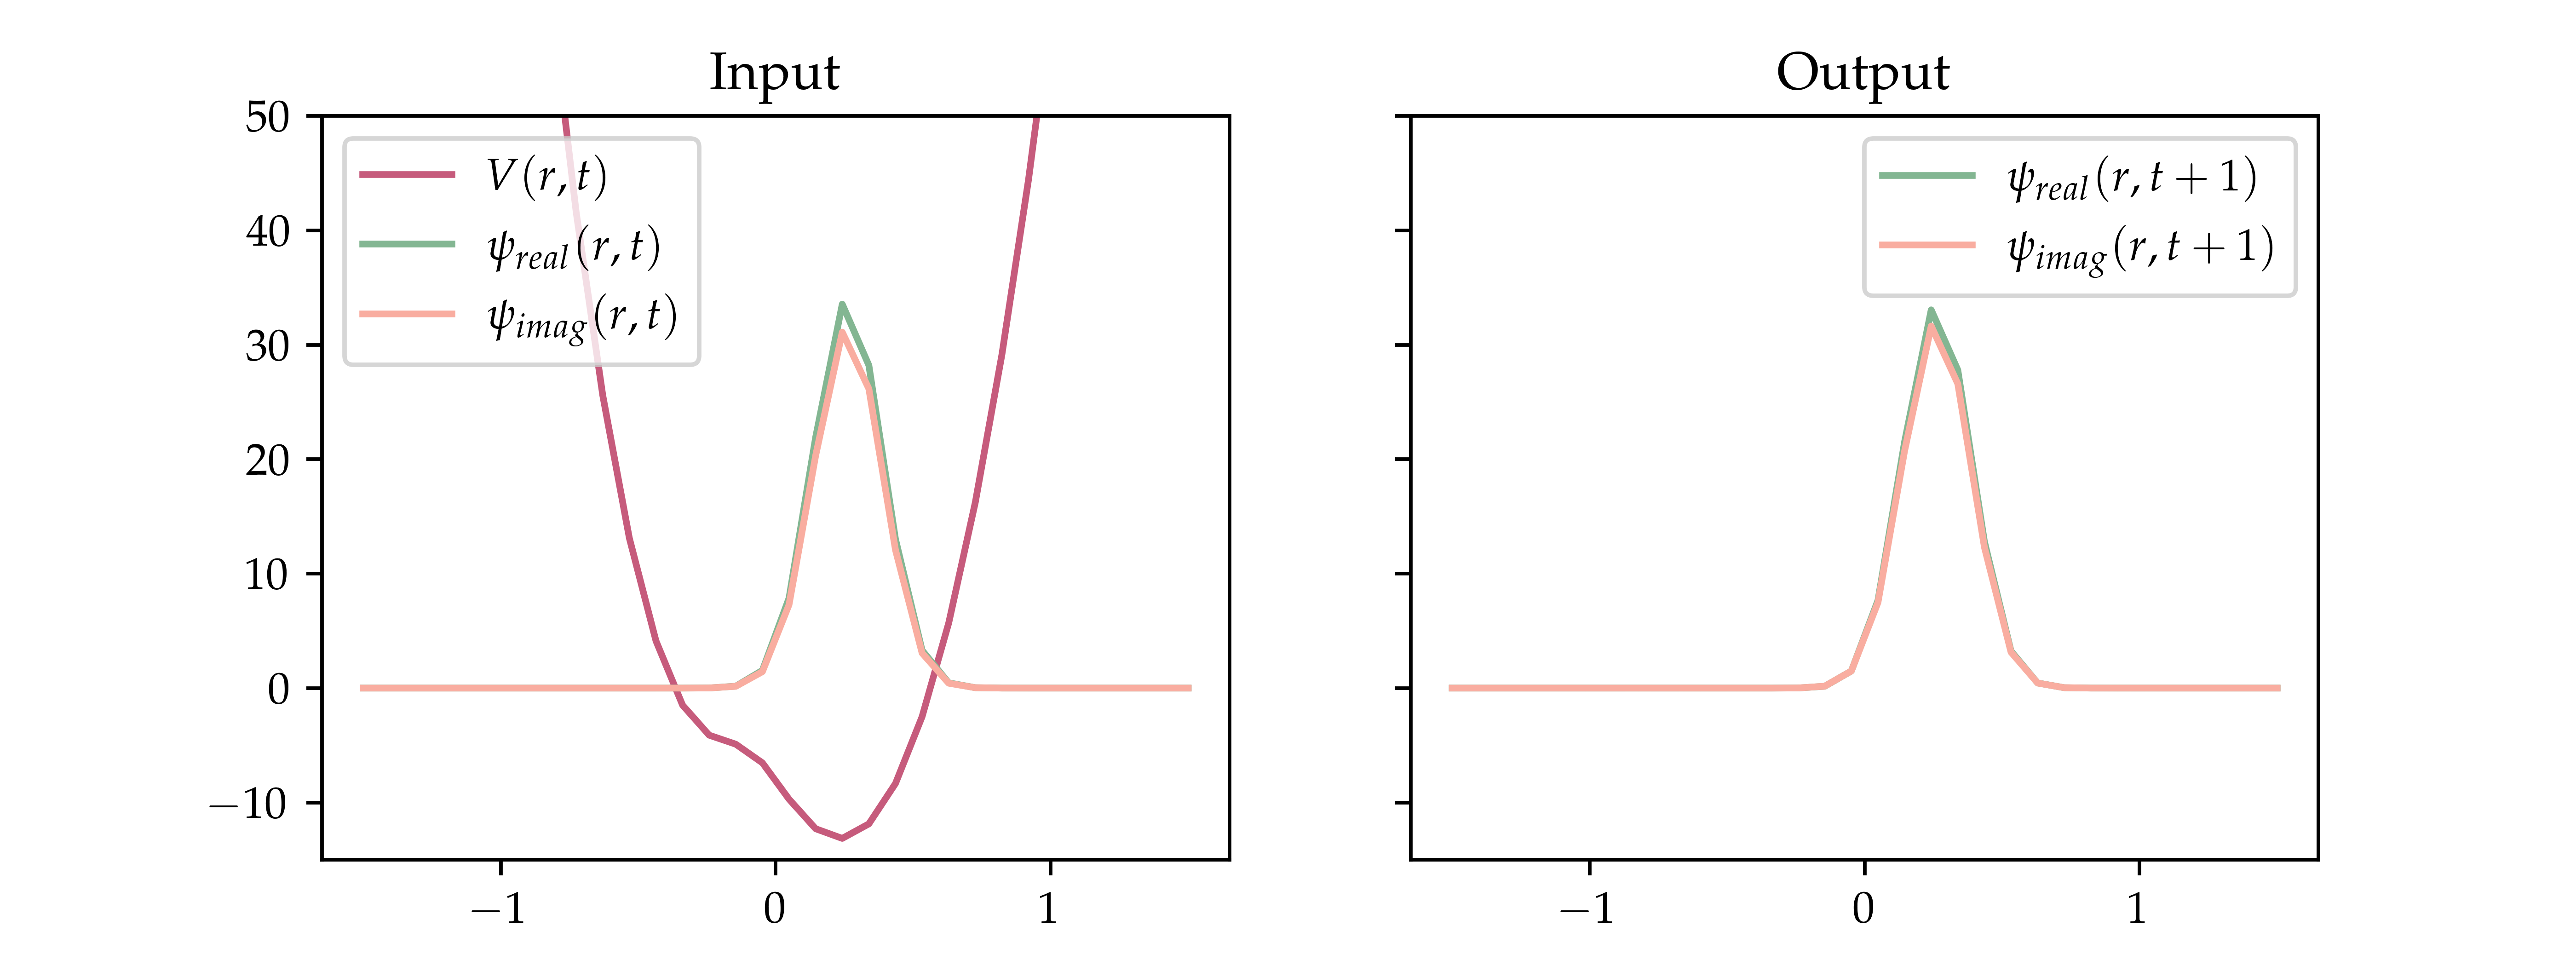
\includegraphics[width=1.3\textwidth]{./img/dataInputOutput.png}}
  \caption{Visualización gráfica: Entrada $X$ y etiqueta $y$ a un tiempo $t$.}
  \label{fig:datavis}
\end{figure}

El código para la preparación de los datos se encuentra en la \href{https://github.com/Jessi-MM/PropagatorLearning/tree/main/Data_Gaussian}{\faGithub Notebook principal} en la clase \texttt{Propagator\_Dataset}.\\
La división de los datos se muestra en la \autoref{tab:SplitData}.

\begin{table}[ht]
  \myfloatalign
  \begin{tabularx}{0.7\textwidth}{XXXX} \toprule
   \tableheadline{Entrenamiento} & \tableheadline{Validación} & \tableheadline{Test} & \tableheadline{Total} \\ \midrule
   5600          &  1600  & 800  & 8000  \\ \midrule
   70\%          &  20\% & 10\% & 100\% \\
    \bottomrule
  \end{tabularx}
  \caption{División de datos}
  \label{tab:SplitData}
\end{table}

\subsection{Modelo LSTM: arquitectura y entrenamiento}\label{sec:6.4.3}

Para el modelo de la red y su entrenamiento se utilizó PyTorch versión 1.9.0+cu102 en una computadora personal. El resumen del modelo se muestra en la \autoref{tab:model}, y el código completo se puede ver en \href{https://github.com/Jessi-MM/LSTM_PropagatorLearning/blob/main/src/Python/LSTM_model.py}{\faGithub Implementación LSTM}.

\begin{table}[ht]
  \myfloatalign
  \begin{tabularx}{\textwidth}{XXX} \toprule
   \tableheadline{Capas} & \tableheadline{Nodos} & \tableheadline{Entrada/Salida} \\ \midrule
   LSTM          &  1024  & (In: 96, Ou:1024)  \\ \midrule
   LSTM          &  1024  & (In: 1024, Ou:1024)  \\ \midrule
   Lineal        &  64    & (In: 1024, Ou:64) \\
   \bottomrule
   Loss Function:      & Mean Square Error \\
   Optimizer:          & AdamW &  weight decay = 0.01 \\
   Batch size:         & 10 \\
   Learning rate:      & 0.0001 \\
   Epochs:             & 290 \\
   \bottomrule
   
  \end{tabularx}
  \caption{Resumen del modelo}
  \label{tab:model}
\end{table}

En donde los parámetros utilizados fueron elegidos después de varios intentos para hallar los que minimizaran la función de pérdida o loss function más rápido, es decir en un menor número de épocas. Las funciones de activación en las capas \acs{LSTM} son las mencionadas en la sección \autoref{sec:lstm}, mientras que la última capa corresponde a una capa lineal debido a que la salida $y$ corresponde a valores reales. El algoritmo de optimización\footnote{Detalles en la sección \autoref{sec:TrainNN}} utiliza una técnica de regularización para prevenir el sobre-entrenamiento, que consiste en agregar una pequeña penalización a la pérdida, que es la norma $L_2$ de todos los pesos entrenables del modelo: \cite{https://doi.org/10.48550/arxiv.1711.05101}

\[ loss = loss + \text{weight decay}*L_2\]

En la \autoref{fig:Model} se muestra un diagrama del modelo de red representado en capas de tiempo (sección \autoref{sec:lstm}), con las entradas y salidas correspondes.

\begin{figure}[!htbp]
  \centering
  \makebox[\textwidth][c]{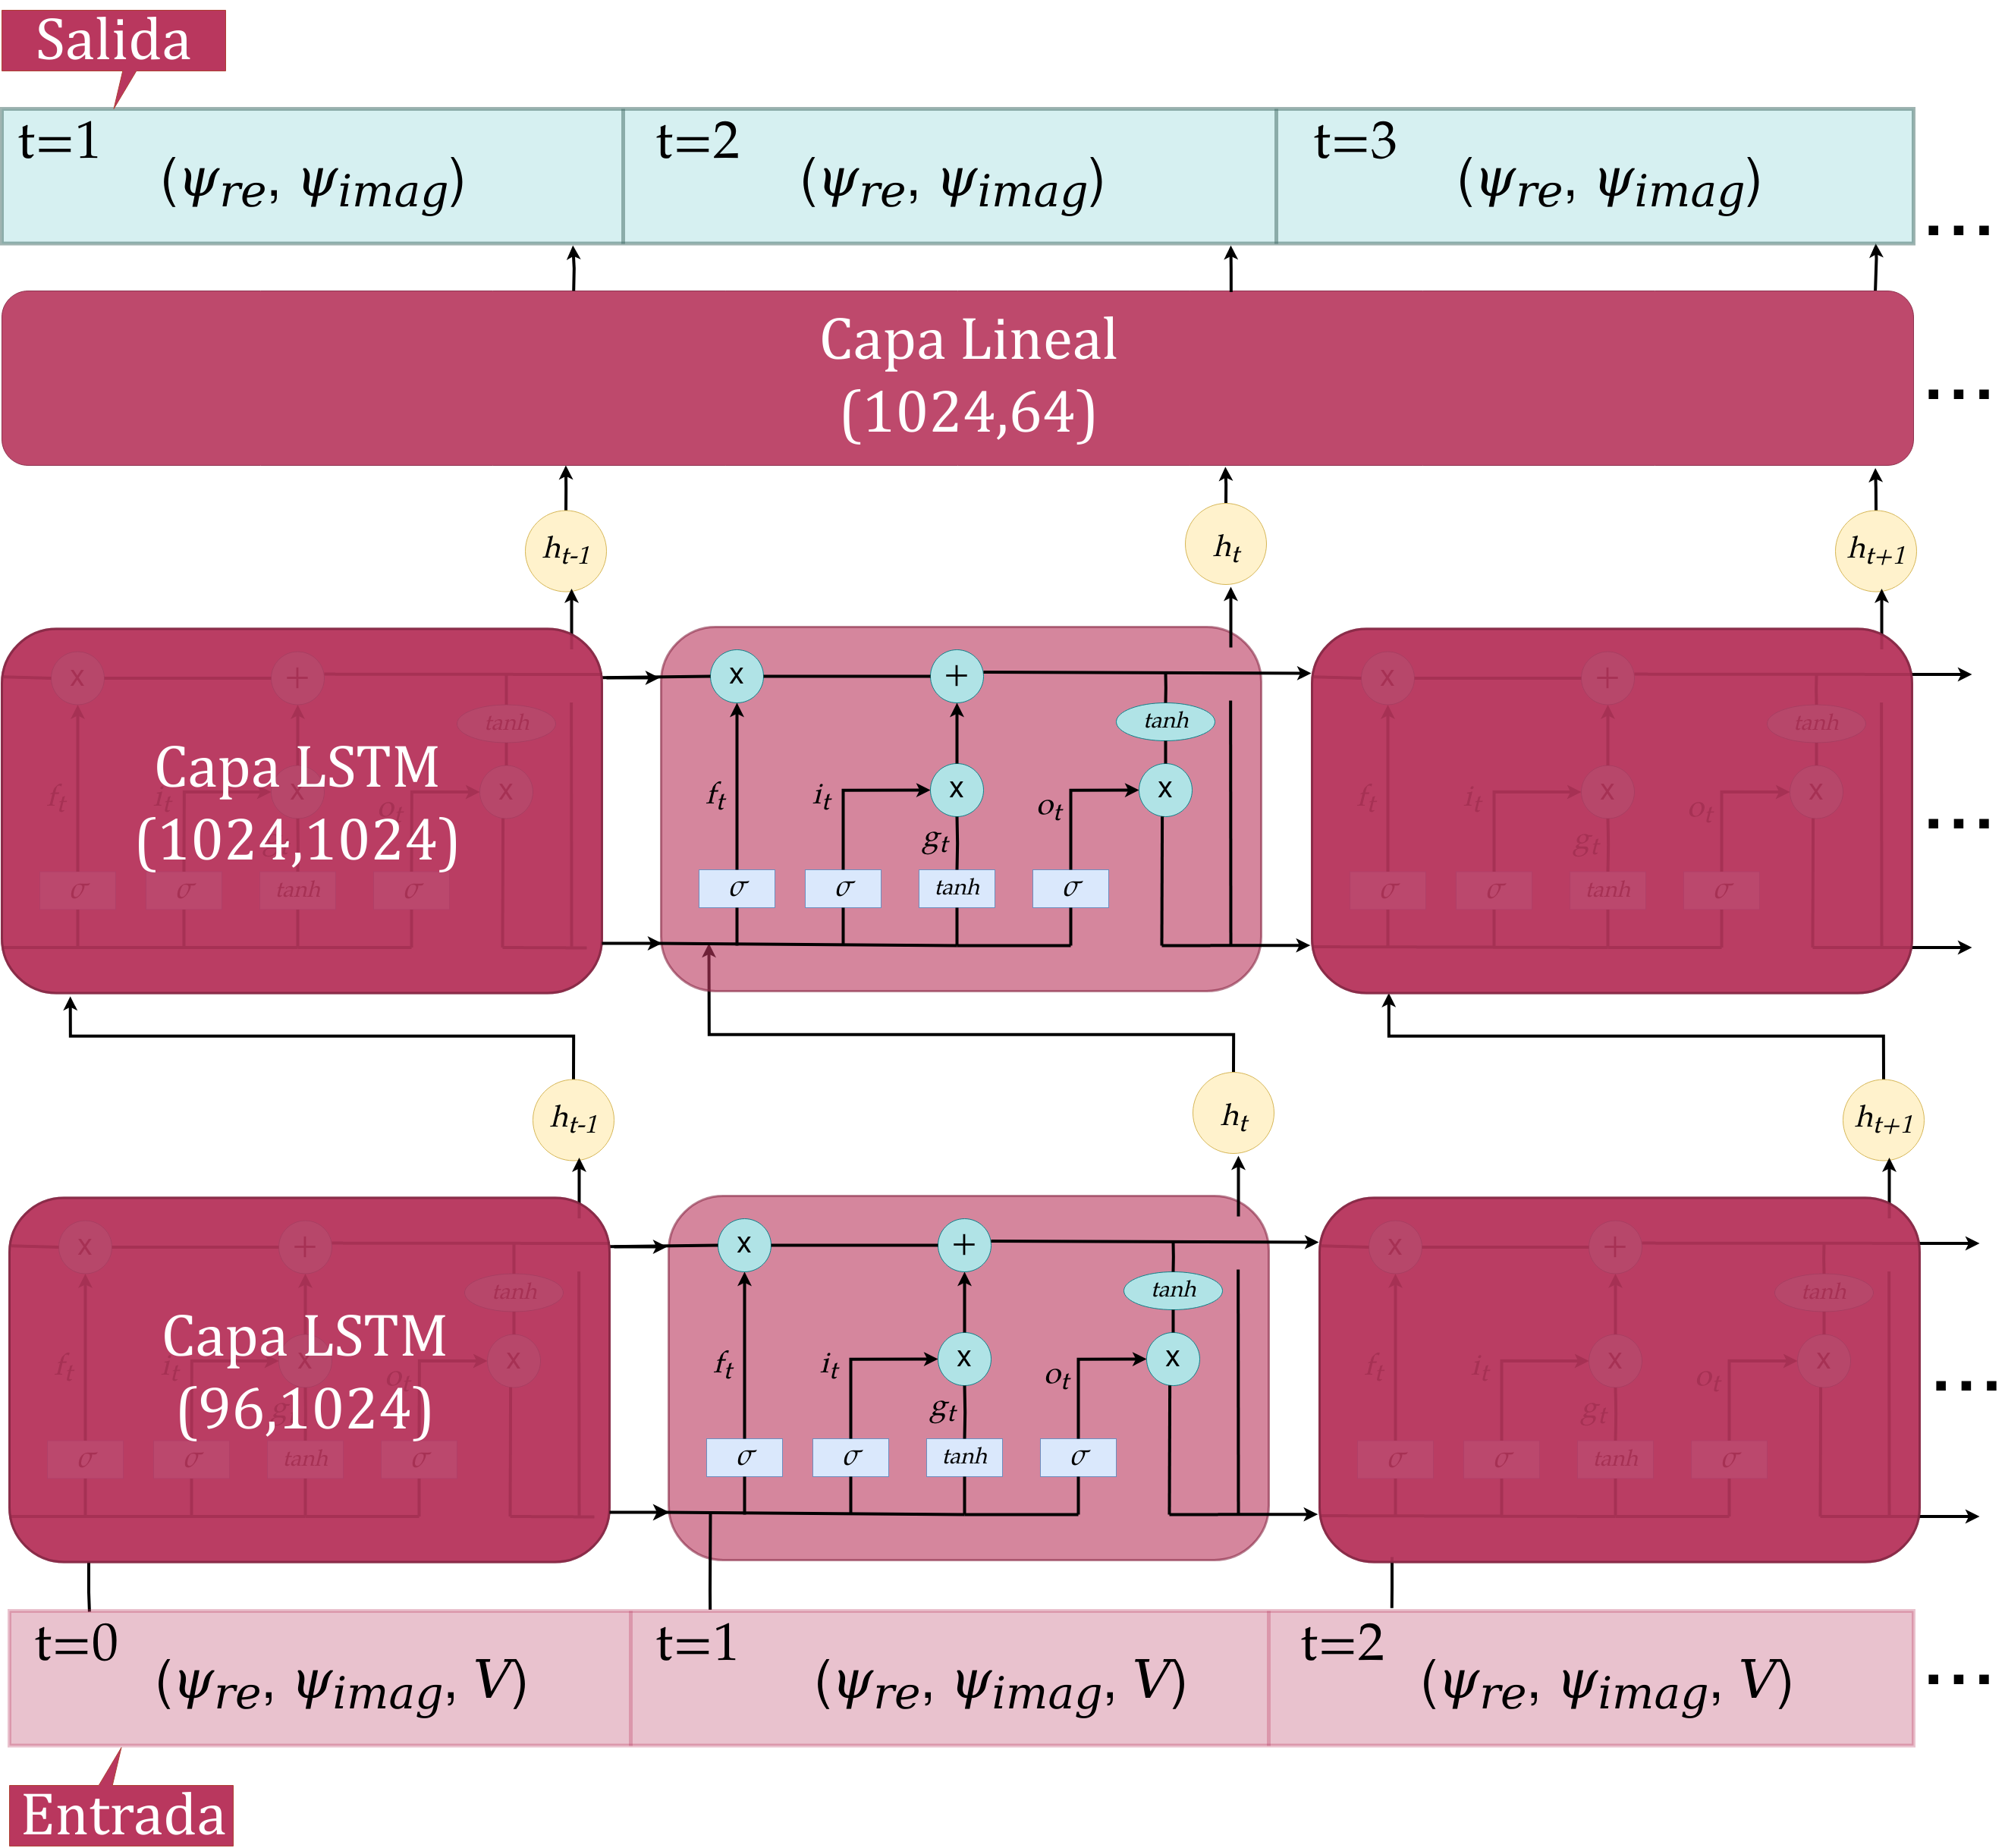
\includegraphics[width=1.3\textwidth]{./img/model/modelDiag2.png}}
  \caption{Diagrama del modelo \acs{LSTM}: se muestran 3 de las 200 capas de tiempo.}
  \label{fig:Model}
\end{figure}

Para calcular la precisión del modelo se utilizó la \autoref{eq:S}:

\begin{equation}
  \label{eq:S}
  S = \bra{\psi_{LSTM}}\ket{\psi_{True}} = |S|\exp{i\theta}
\end{equation}

que compara dos funciones de onda, la predicha por el modelo $\psi_{LSTM}$ respecto a la esperada $\psi_{True}$, cuando se trata de la misma función de onda, dado que están normalizadas, se sigue que:
\begin{equation*}
  \bra{\psi}\ket{\psi} = \int_{a}^{b}\psi(x) \psi(x)^\dag dx = \int_{a}^{b}|\psi(x)| dx = 1 = |S|\exp{i\theta}
\end{equation*}

$\iff |S|=1$ y $\theta =0$. Es decir, que la función de onda $\psi_{LSTM}$ predicha por el modelo es más parecida a la esperada $\psi_{True}$ cuanto más se acerca $|S|$ a $1$ y $\theta$ a $0$. \\

Al finalizar cada época en el entrenamiento se calculó la función de precisión para cada onda en cada trayectoria en el conjunto de validación y se promediaron los valores correspondientes a $|S|$ y $\theta$. 

\subsection{Resultados y análisis: precisión y predicciones}\label{sec:Resultados}

En la \autoref{fig:S-phase} se muestran los valores promedio obtenidos de la magnitud absoluta $|S|$ y la fase $\theta$ a través de las épocas.

\begin{figure}[!htbp]
  \centering
  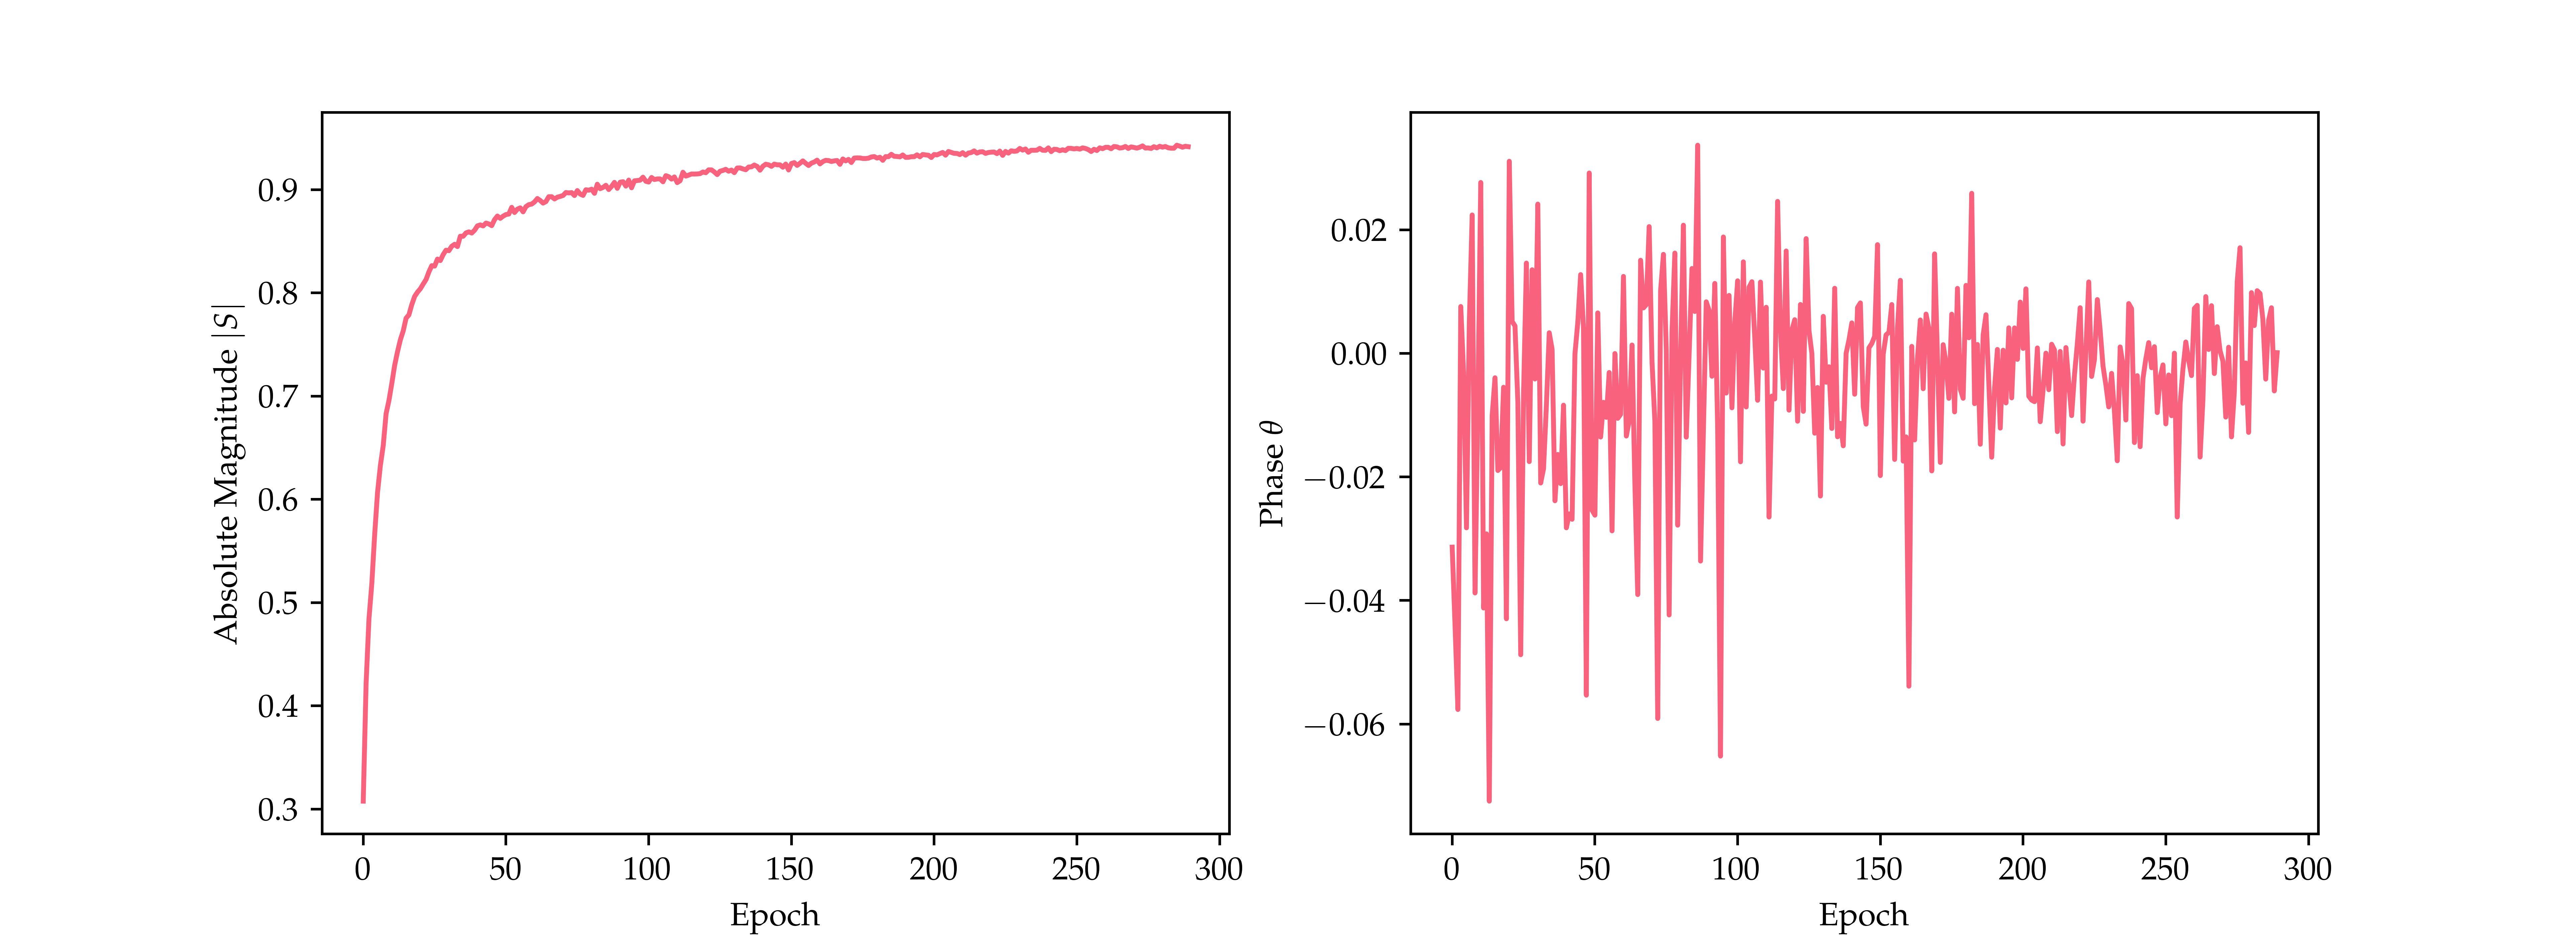
\includegraphics[width=1\textwidth]{./img/S-plot.png}
  \caption{Valores promedio de $|S|$ y $\theta$ en el conjunto de validación por cada época.}
  \label{fig:S-phase}
\end{figure}

Al finalizar el entrenamiento, sobre el conjunto de testeo los resultados de las variables se reportan en la \autoref{tab:res-S}.

\begin{table}[ht]
  \myfloatalign
  \begin{tabularx}{0.3\textwidth}{XX} \toprule
   \tableheadline{$|S|$} & \tableheadline{$\theta$} \\ \midrule
   0.946          &  0.0001 \\
   \bottomrule  
  \end{tabularx}
  \caption{Valores promedio de $|S|$ y $\theta$ en el conjunto de testeo}
  \label{tab:res-S}
\end{table}

A continuación se muestran algunos ejemplos de predicciones de un solo paso del tiempo tomados aleatoriamente de distintas trayectorias. Los potenciales $V(r,t)$ y funciones de onda iniciales $\psi(r,t=0)$ se tomaron del conjunto de testeo.

\begin{figure}[H]
  \centering
  \makebox[\textwidth][c]{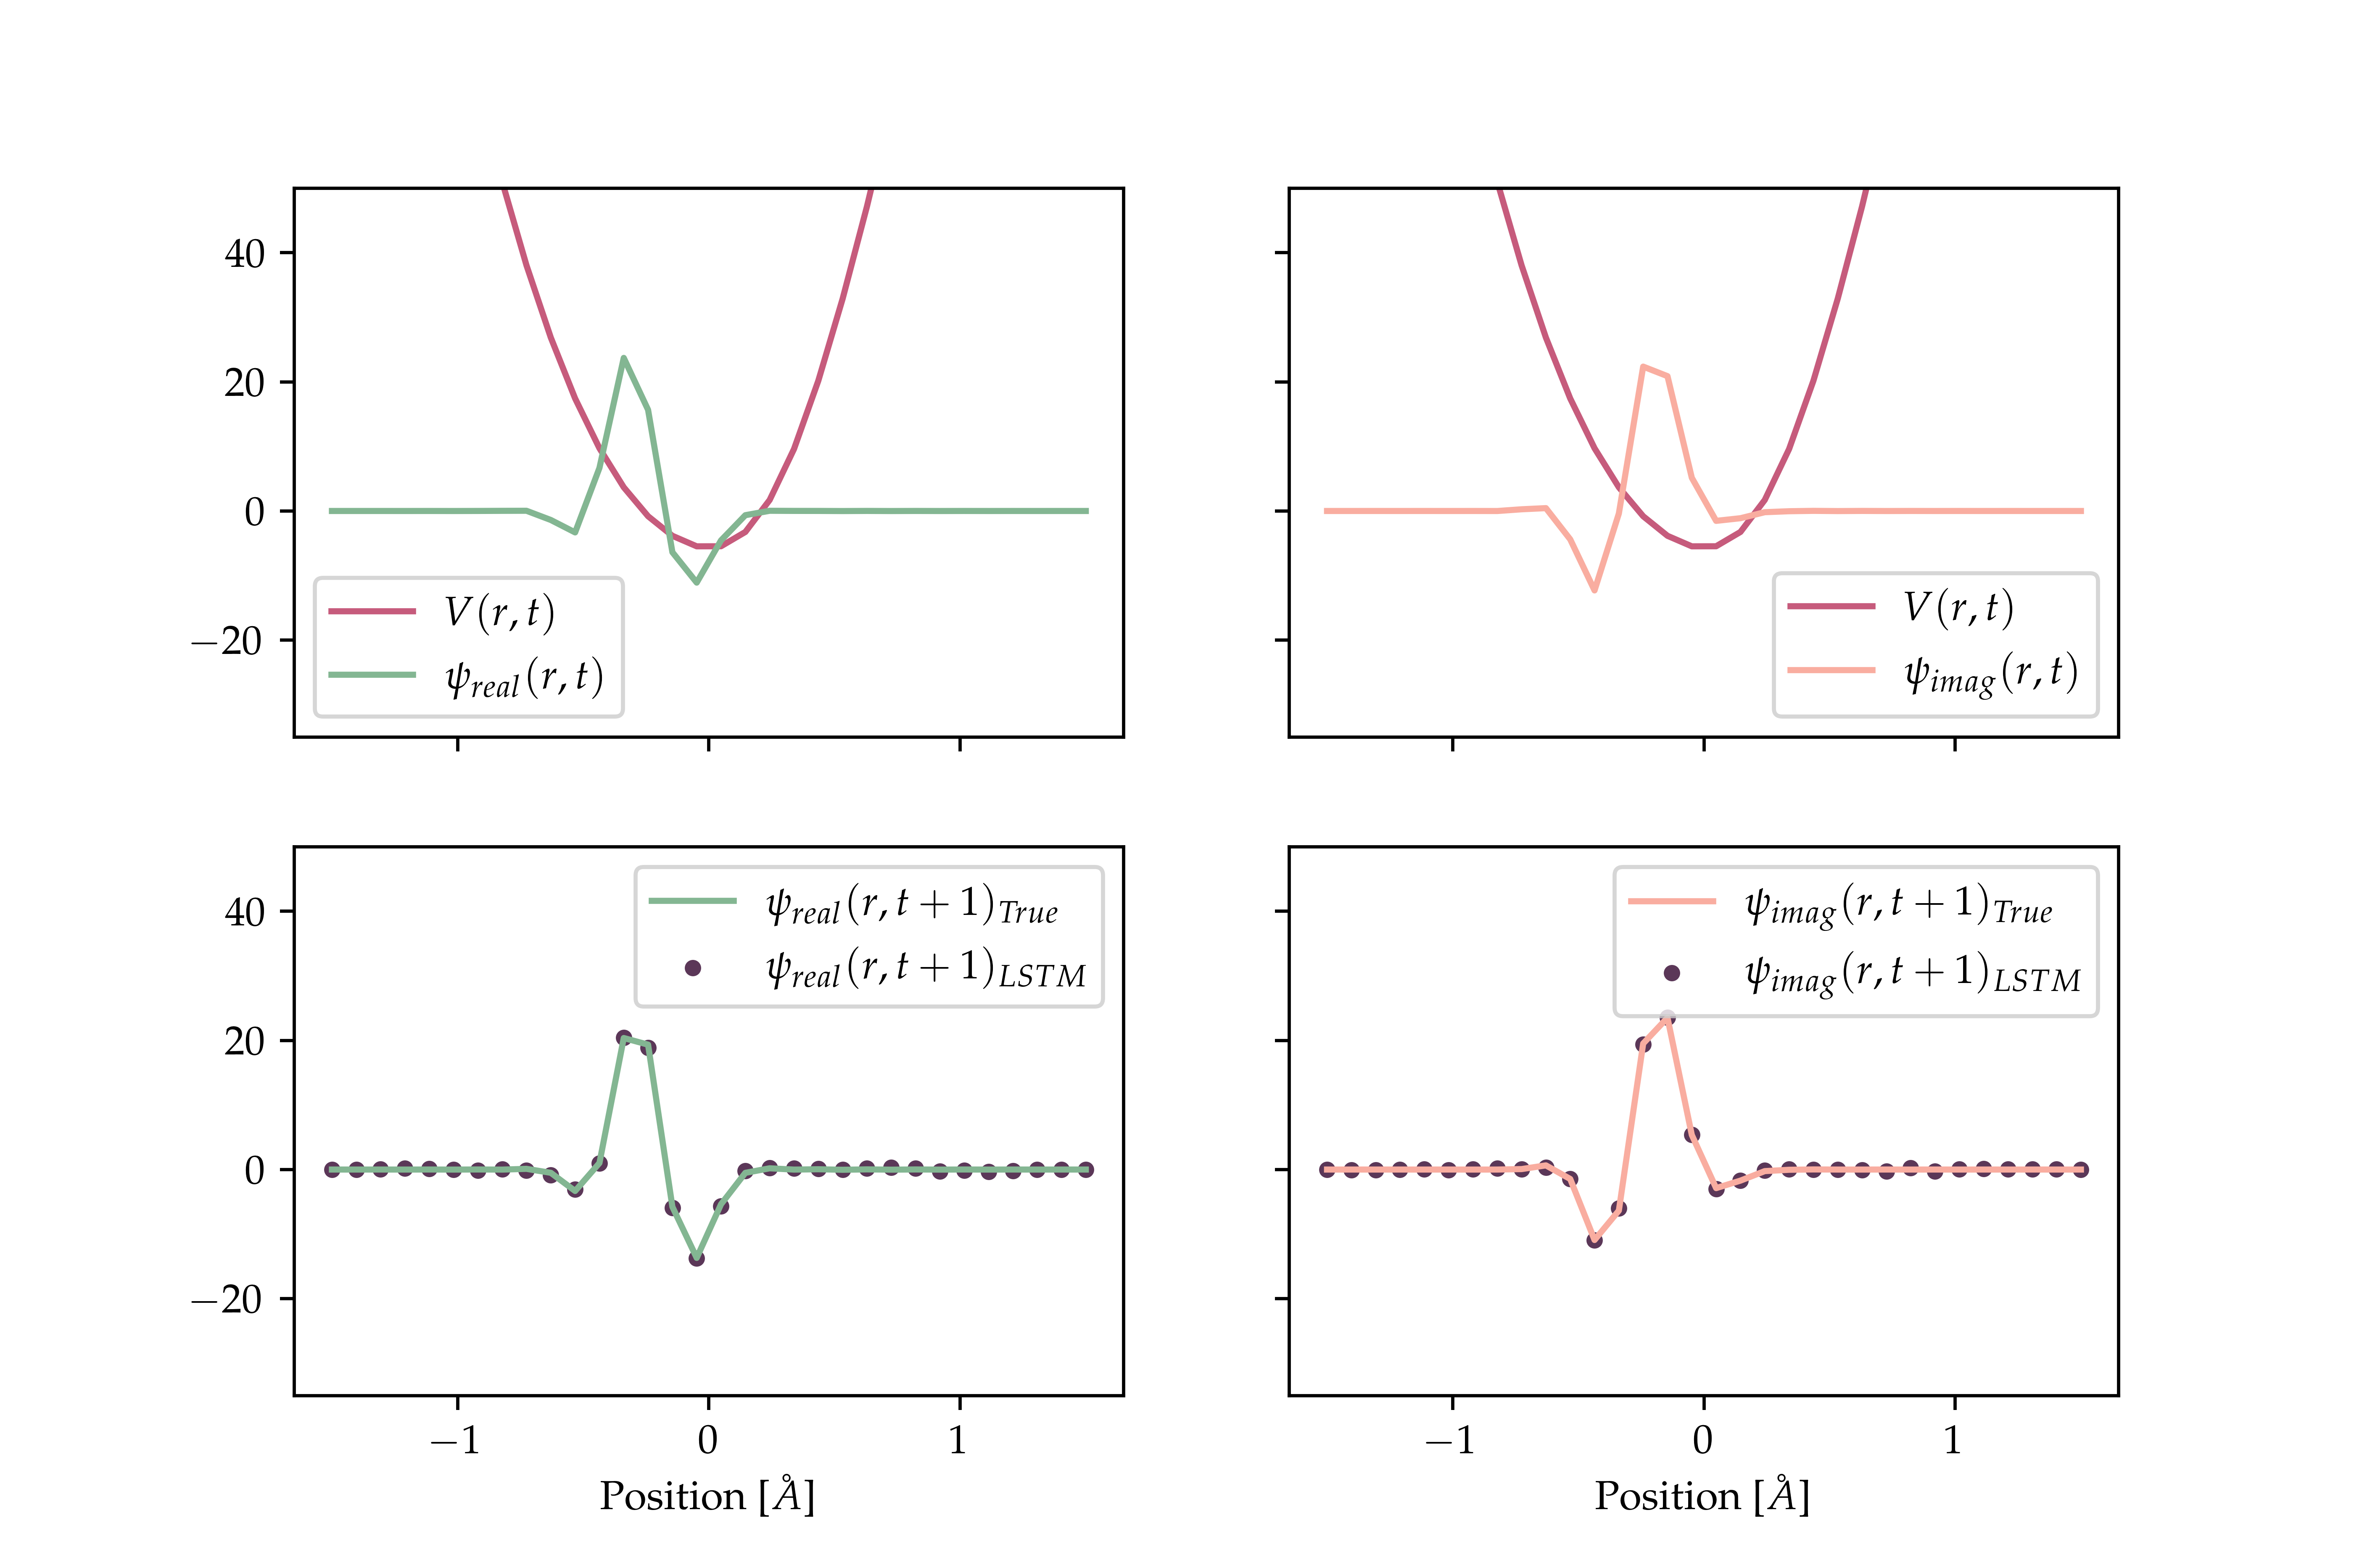
\includegraphics[width=1\textwidth]{./img/model/1step.png}}
  \caption{Ejemplo 1 de predicción a un paso de tiempo $\Delta t = 1\,fs$.\\ Las funciones de onda $\psi$ están escaladas para poder visualizar el potencial en la misma gráfica.}
  \label{fig:1step1}
\end{figure}

\begin{figure}[H]
  \centering
  \makebox[\textwidth][c]{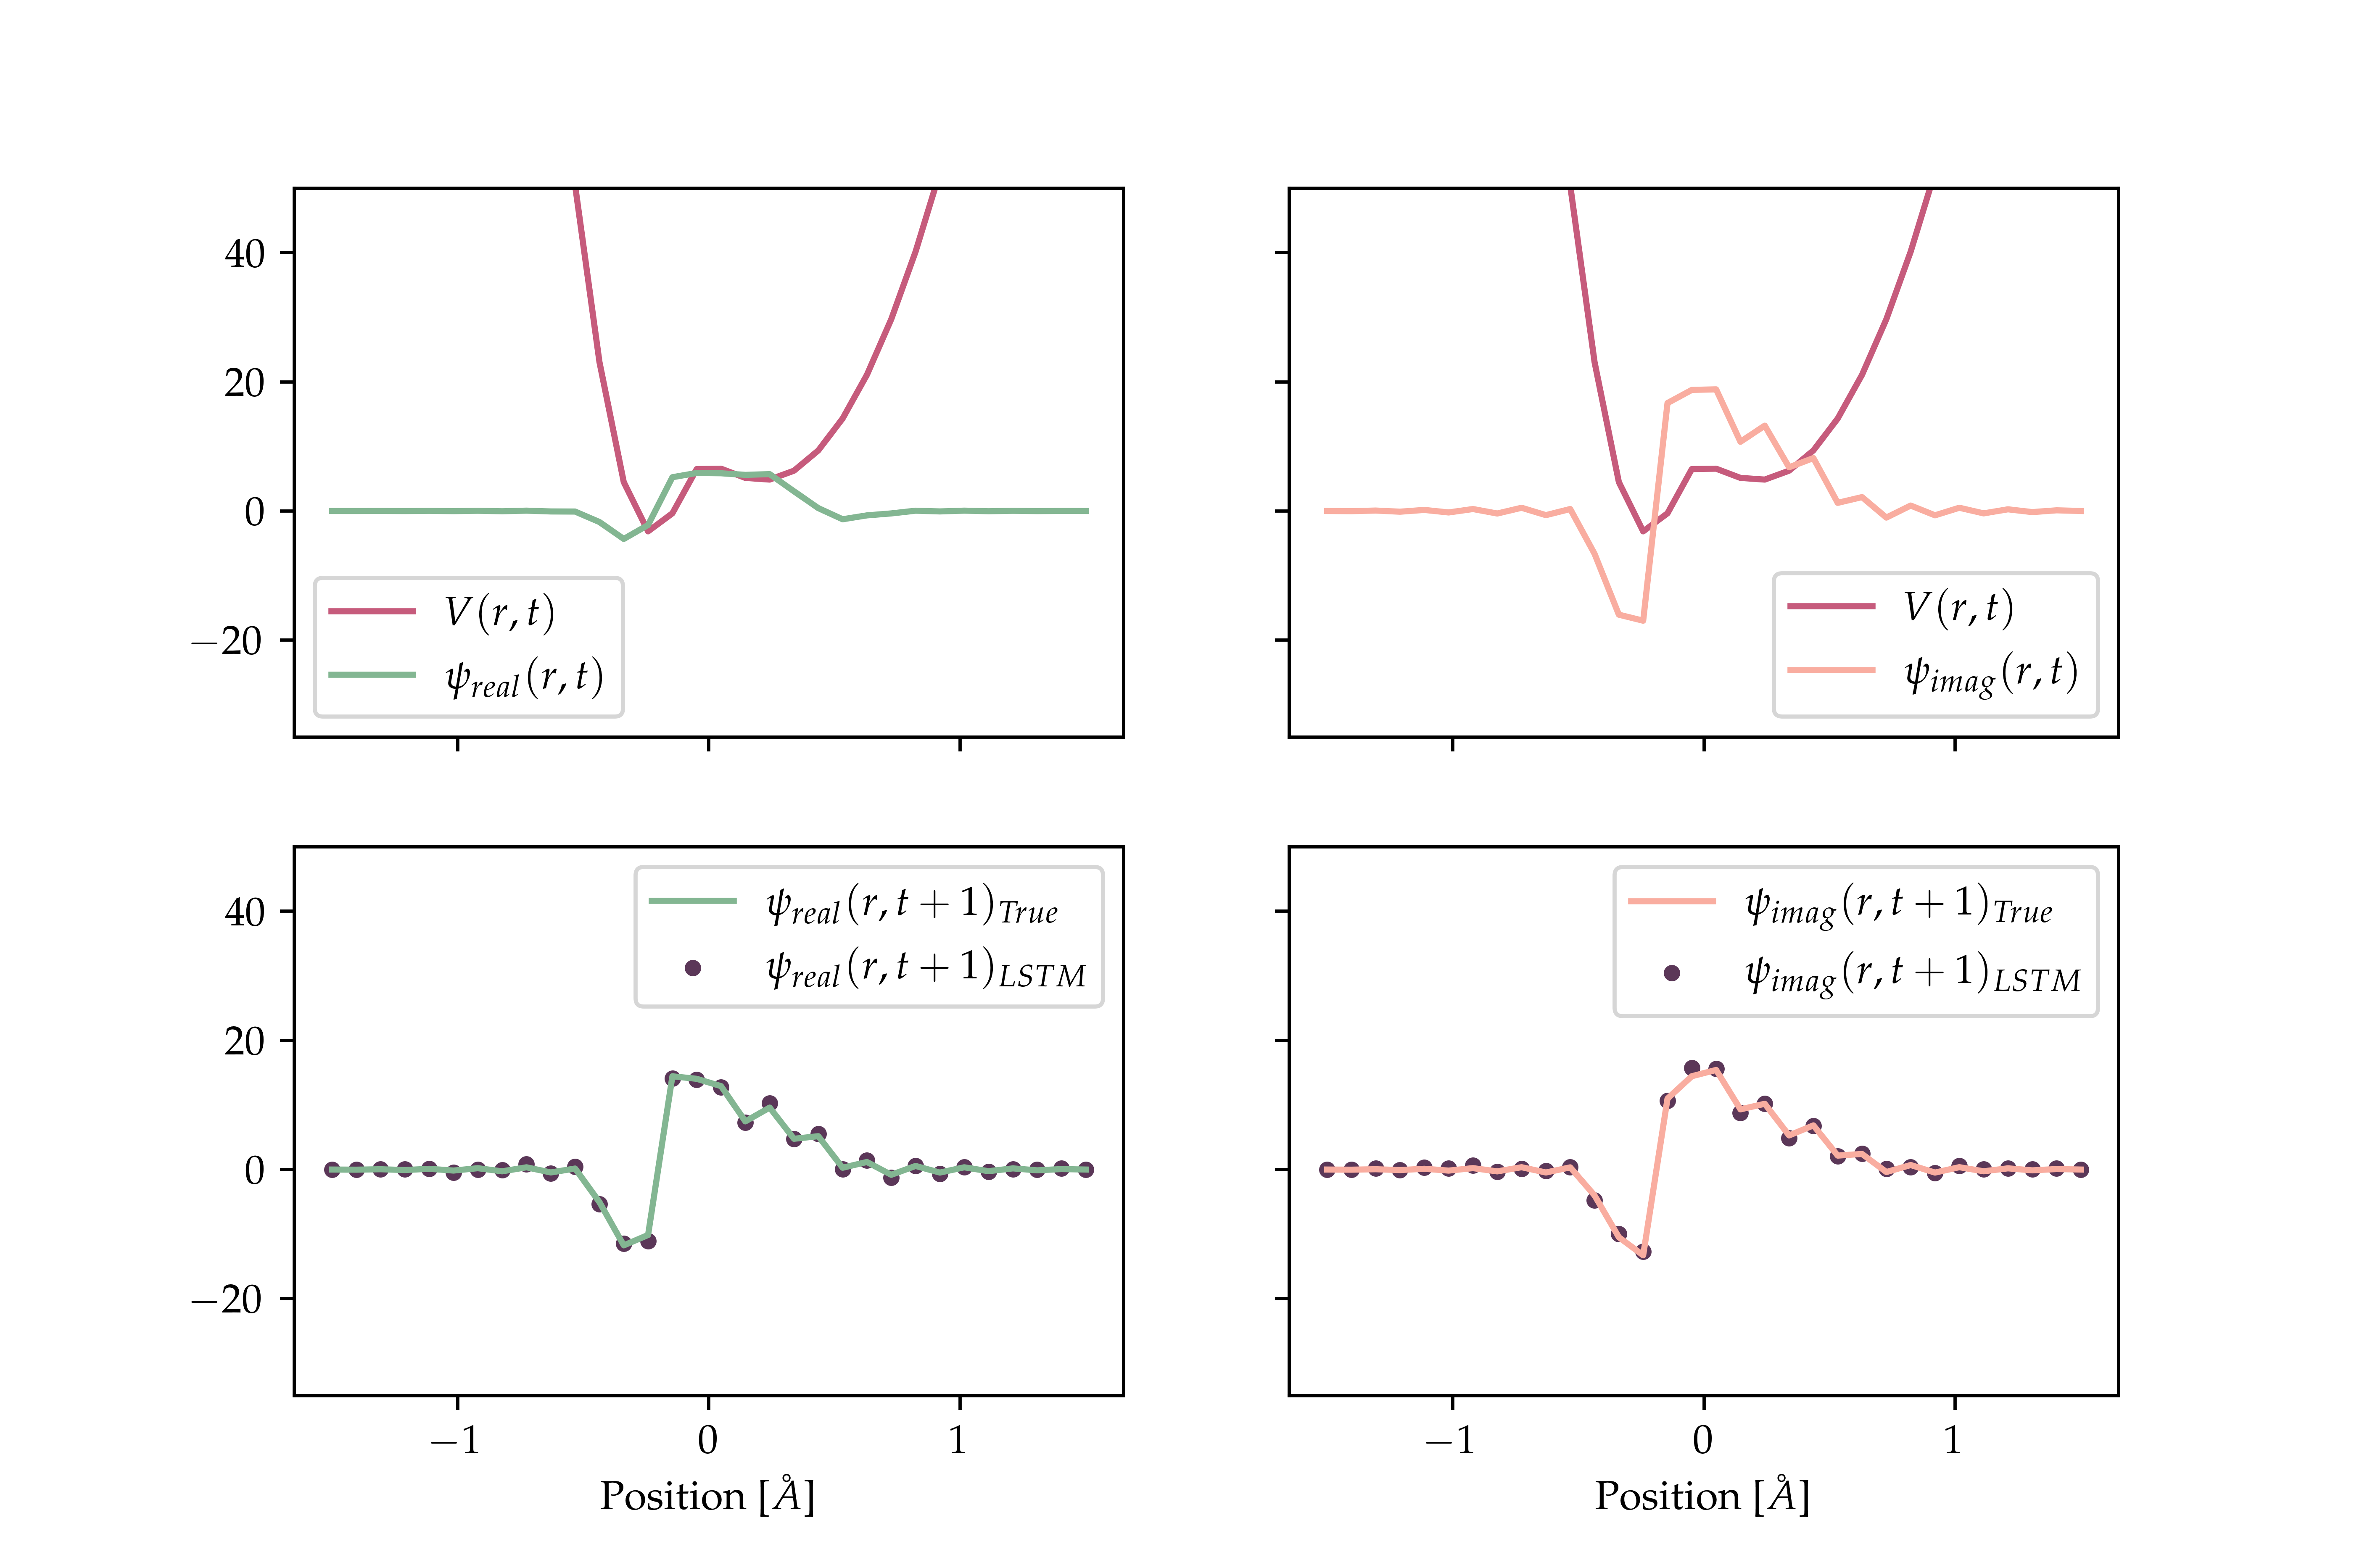
\includegraphics[width=1\textwidth]{./img/model/1step1.png}}
  \caption{Ejemplo 2 de predicción a un paso de tiempo $\Delta t = 1\,fs$.\\ Las funciones de onda $\psi$ están escaladas para poder visualizar el potencial en la misma gráfica.}
  \label{fig:1step2}
\end{figure}

\begin{figure}[H]
  \centering
  \makebox[\textwidth][c]{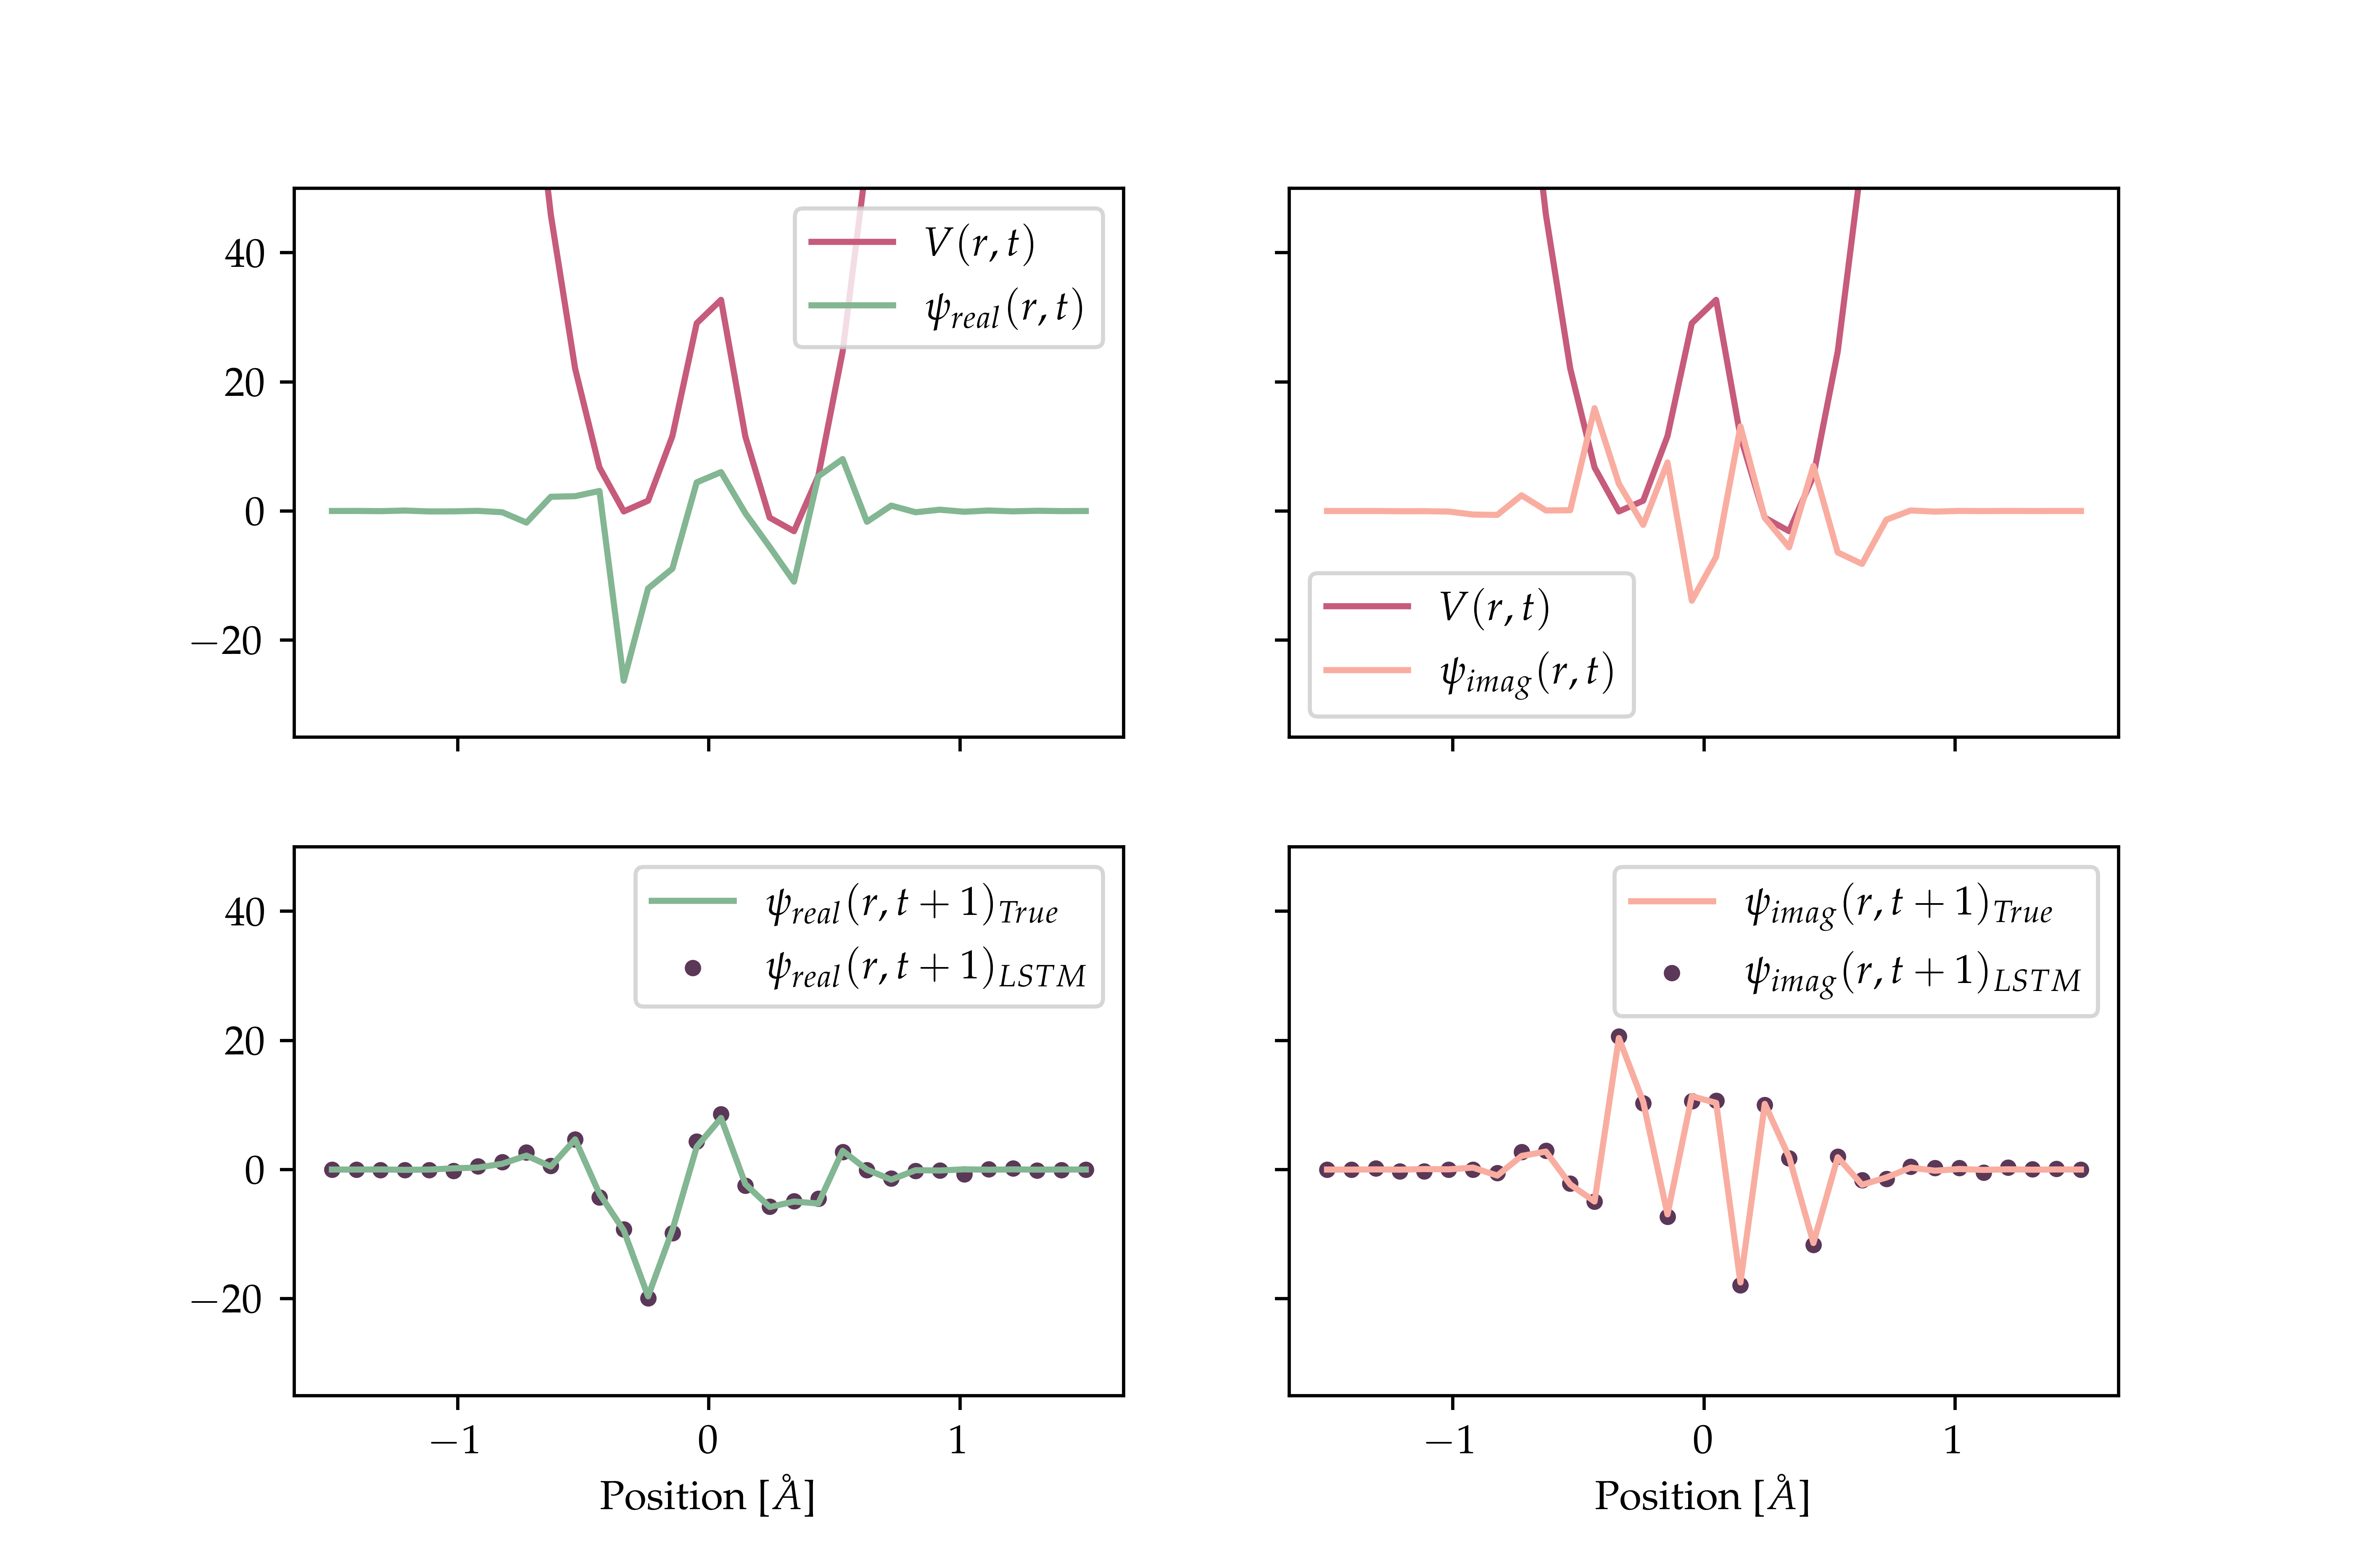
\includegraphics[width=1\textwidth]{./img/model/1step2.png}}
  \caption{Ejemplo 3 de predicción a un paso de tiempo $\Delta t = 1\,fs$.\\ Las funciones de onda $\psi$ están escaladas para poder visualizar el potencial en la misma gráfica. }
  \label{fig:1step3}
\end{figure}

\begin{figure}[!htbp]
  \centering
  \makebox[\textwidth][c]{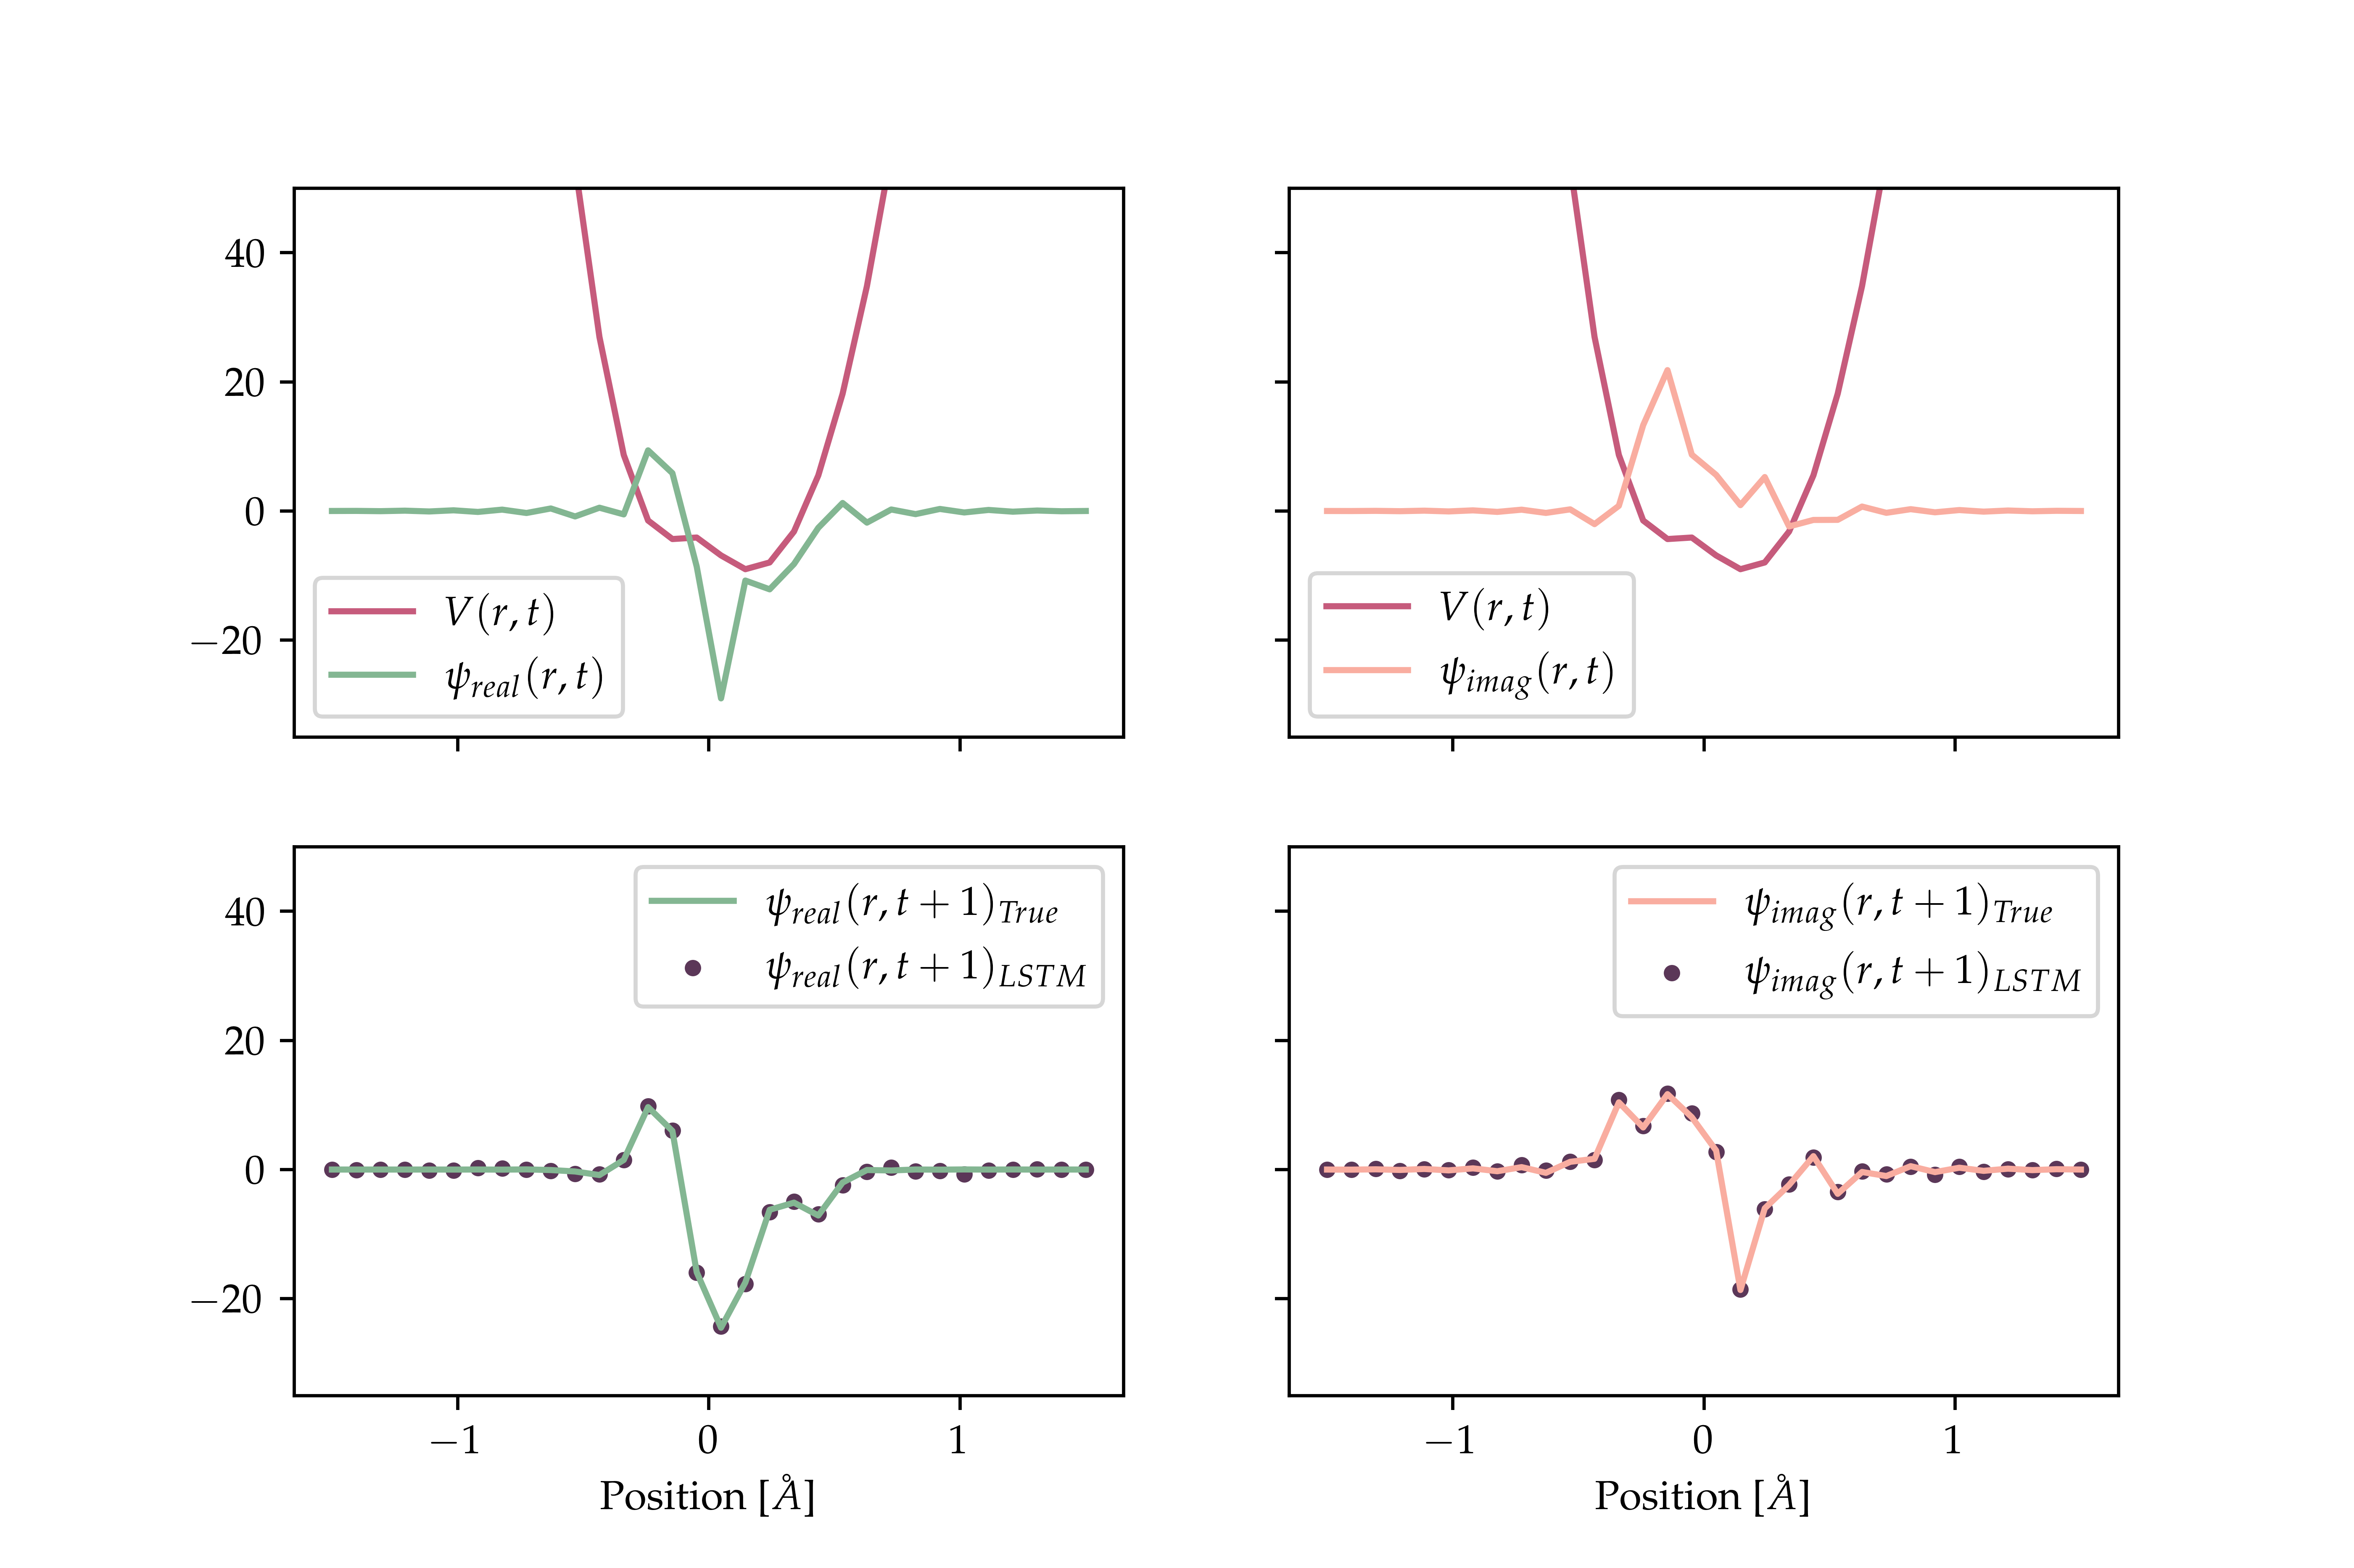
\includegraphics[width=1\textwidth]{./img/model/1step3.png}}
  \caption{Ejemplo 4 de predicción a un paso de tiempo $\Delta t = 1\,fs$.\\ Las funciones de onda $\psi$ están escaladas para poder visualizar el potencial en la misma gráfica.}
  \label{fig:1step4}
\end{figure}

\begin{figure}[H]
  \centering
  \makebox[\textwidth][c]{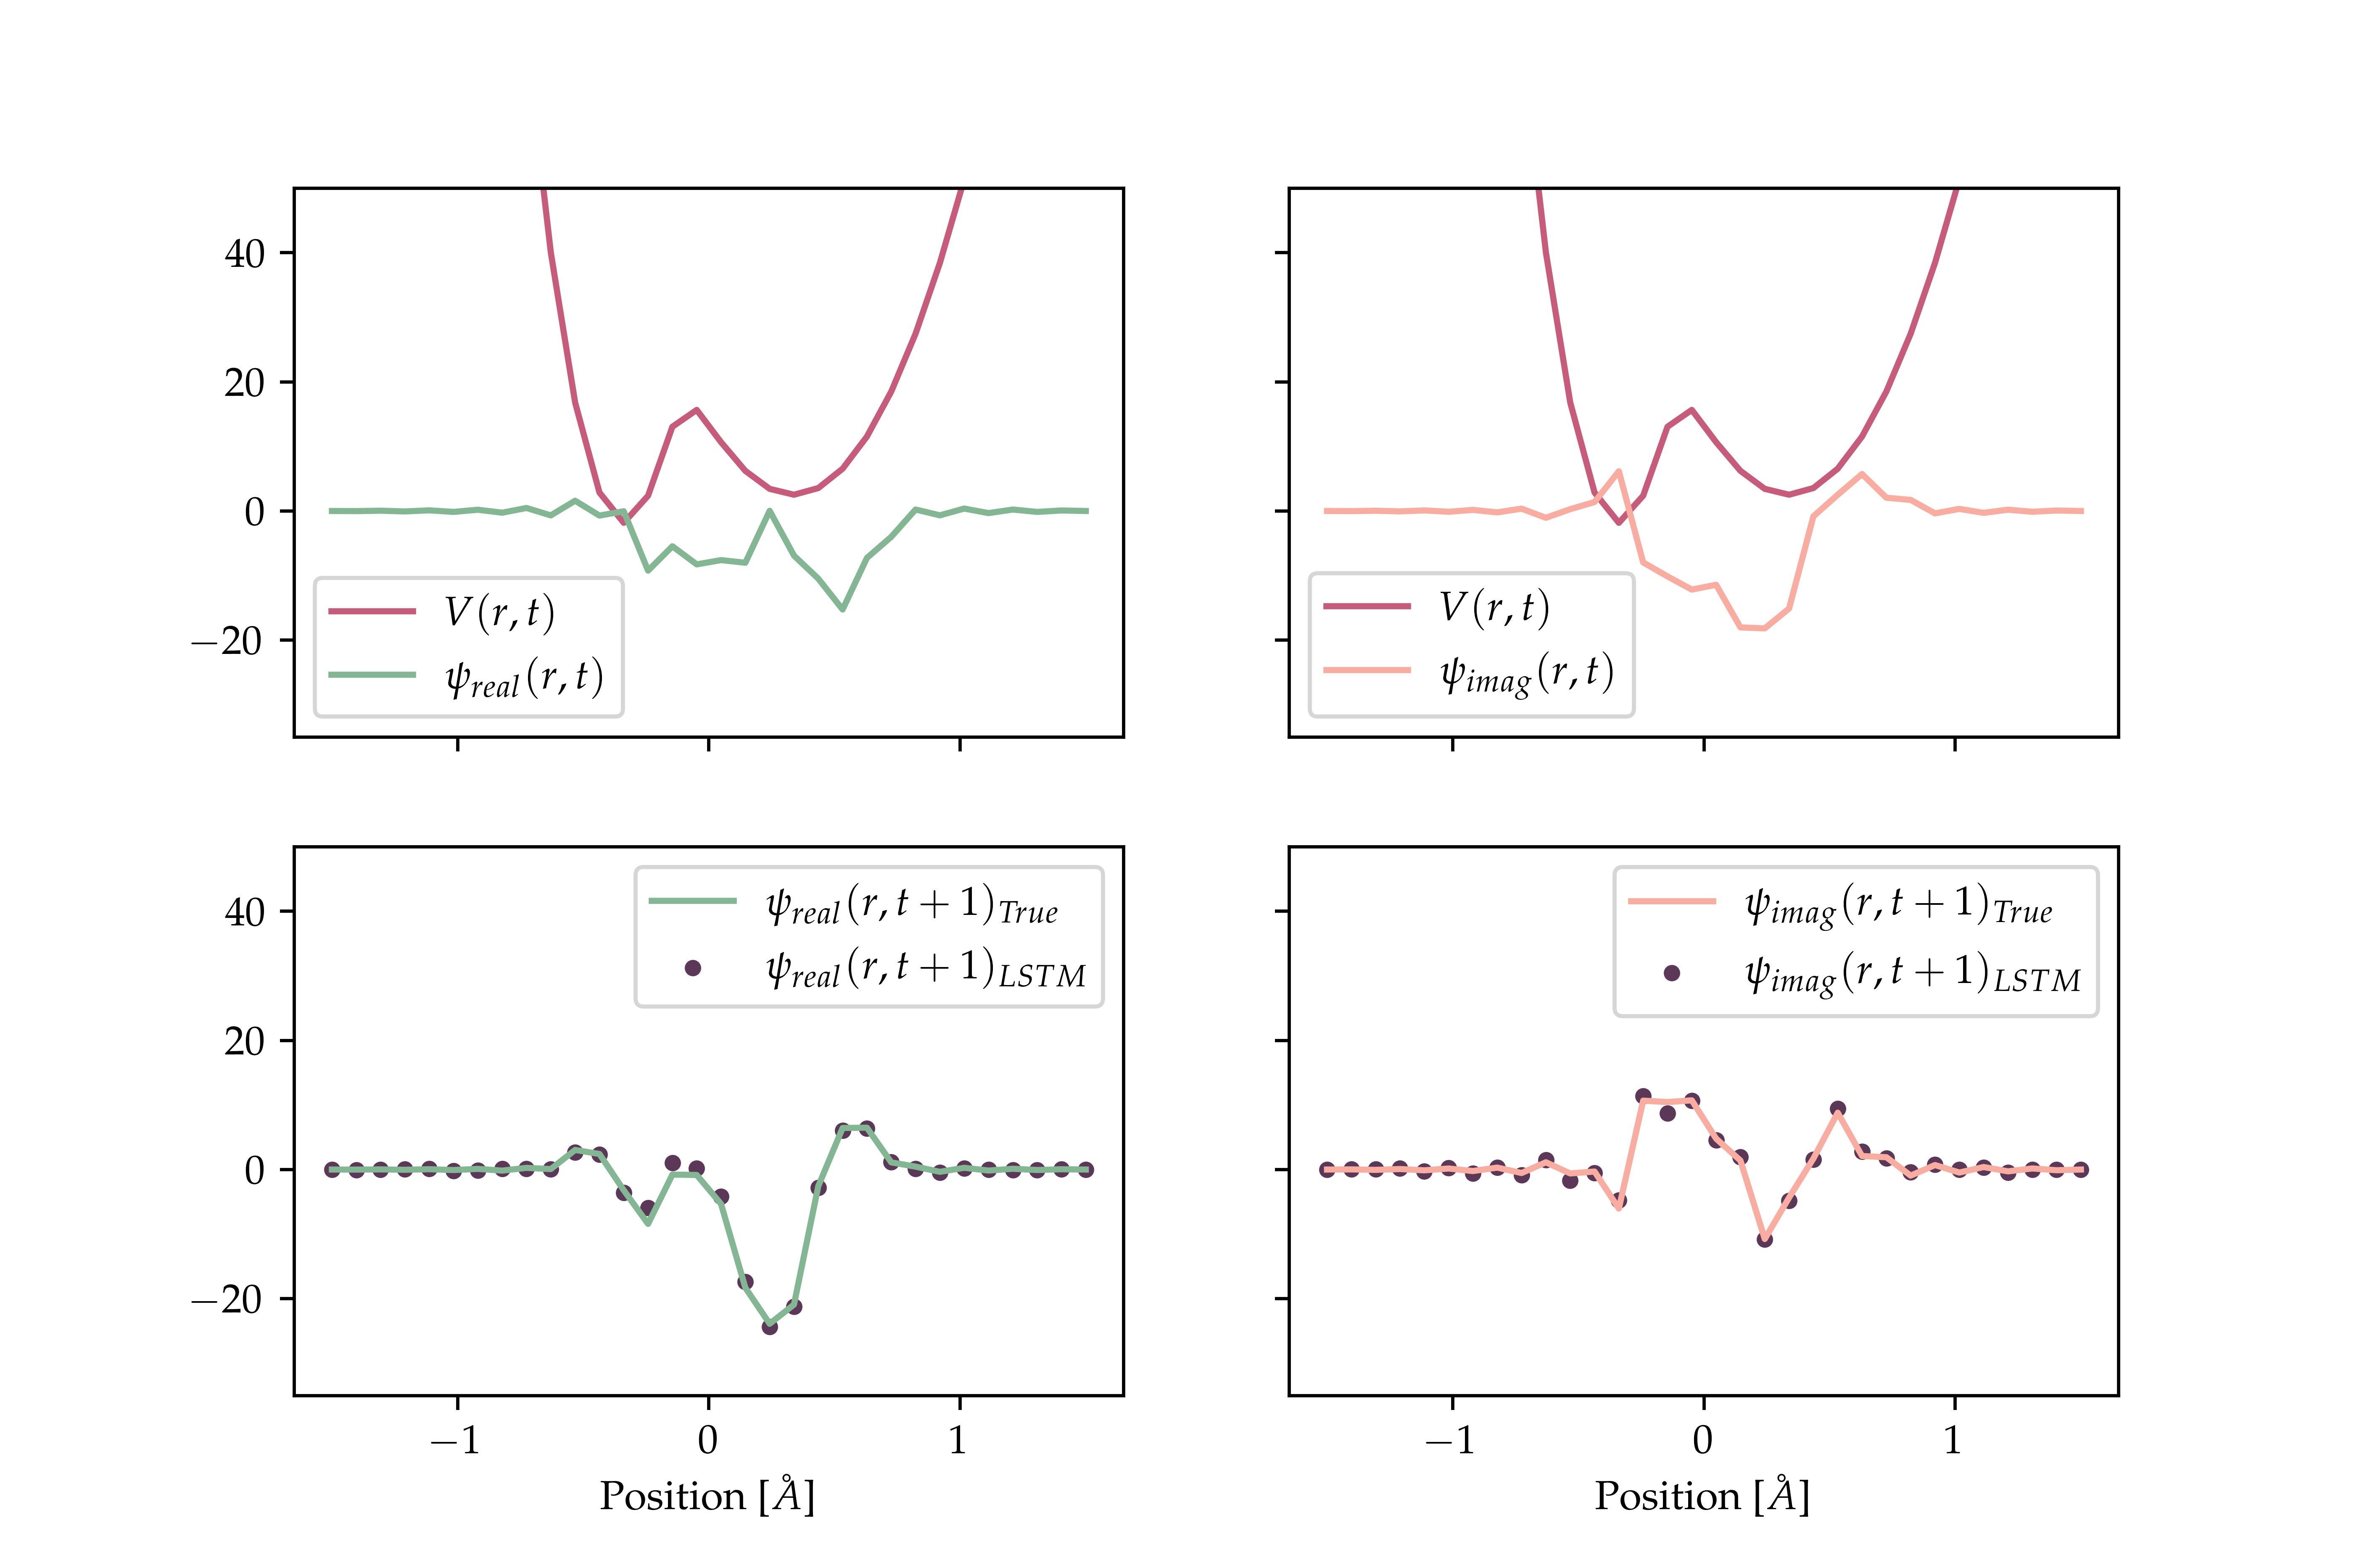
\includegraphics[width=1\textwidth]{./img/model/1step4.png}}
  \caption{Ejemplo 5 de predicción a un paso de tiempo $\Delta t = 1\,fs$.\\ Las funciones de onda $\psi$ están escaladas para poder visualizar el potencial en la misma gráfica.}
  \label{fig:1step5}
\end{figure}

En la \autoref{tab:comptime} se reportan los tiempos de computación requeridos para propagar un paso de tiempo una onda usando los métodos numéricos que utiliza el método \acs{DVR}: la exponenciación o la diagonalización \cite{Main:2021}, y el tiempo requerido que utiliza la red \acs{LSTM} entrenada. 

\begin{table}[H]
  \myfloatalign
  \begin{tabularx}{\textwidth}{XXXX} \toprule
   \tableheadline{N malla} & \tableheadline{exponencial$^a$} & \tableheadline{diagonalización$^b$}& \tableheadline{LSTM$^c$} \\ \midrule
   32          &  0.41 s & 0.14 s & 0.0536 s
 \end{tabularx}
 \begin{tabularx}{\textwidth}{X}
   $^a$Tiempo necesario para realizar la exponenciación matricial del hamiltoniano y multiplicación de matrices para la propagación de paquetes de ondas. $^b$Tiempo requerido para realizar la diagonalización de matrices, multiplicación de vectores por elementos, y transformación de base. $^c$Tiempo necesario para aplicar la red LSTM entrenada para la propagación de paquetes de ondas. \\
   \bottomrule  
  \end{tabularx}
  \caption{Tiempo requerido para propagar un paquete de onda un paso en el tiempo $\Delta t$}
  \label{tab:comptime}
\end{table}



Las siguientes gráficas muestran la evolución temporal de la densidad de probabilidad $|\psi(r,t)|$ a través del tiempo bajo potenciales $V(r,t)$ calculadas utilizando la función de onda predicha por la red. Los potenciales $V(r,t)$ y funciones de onda iniciales $\psi(r,t=0)$ se tomaron del conjunto de testeo.

\newpage

\begin{figure}[H]
  \centering
  \makebox[\textwidth][c]{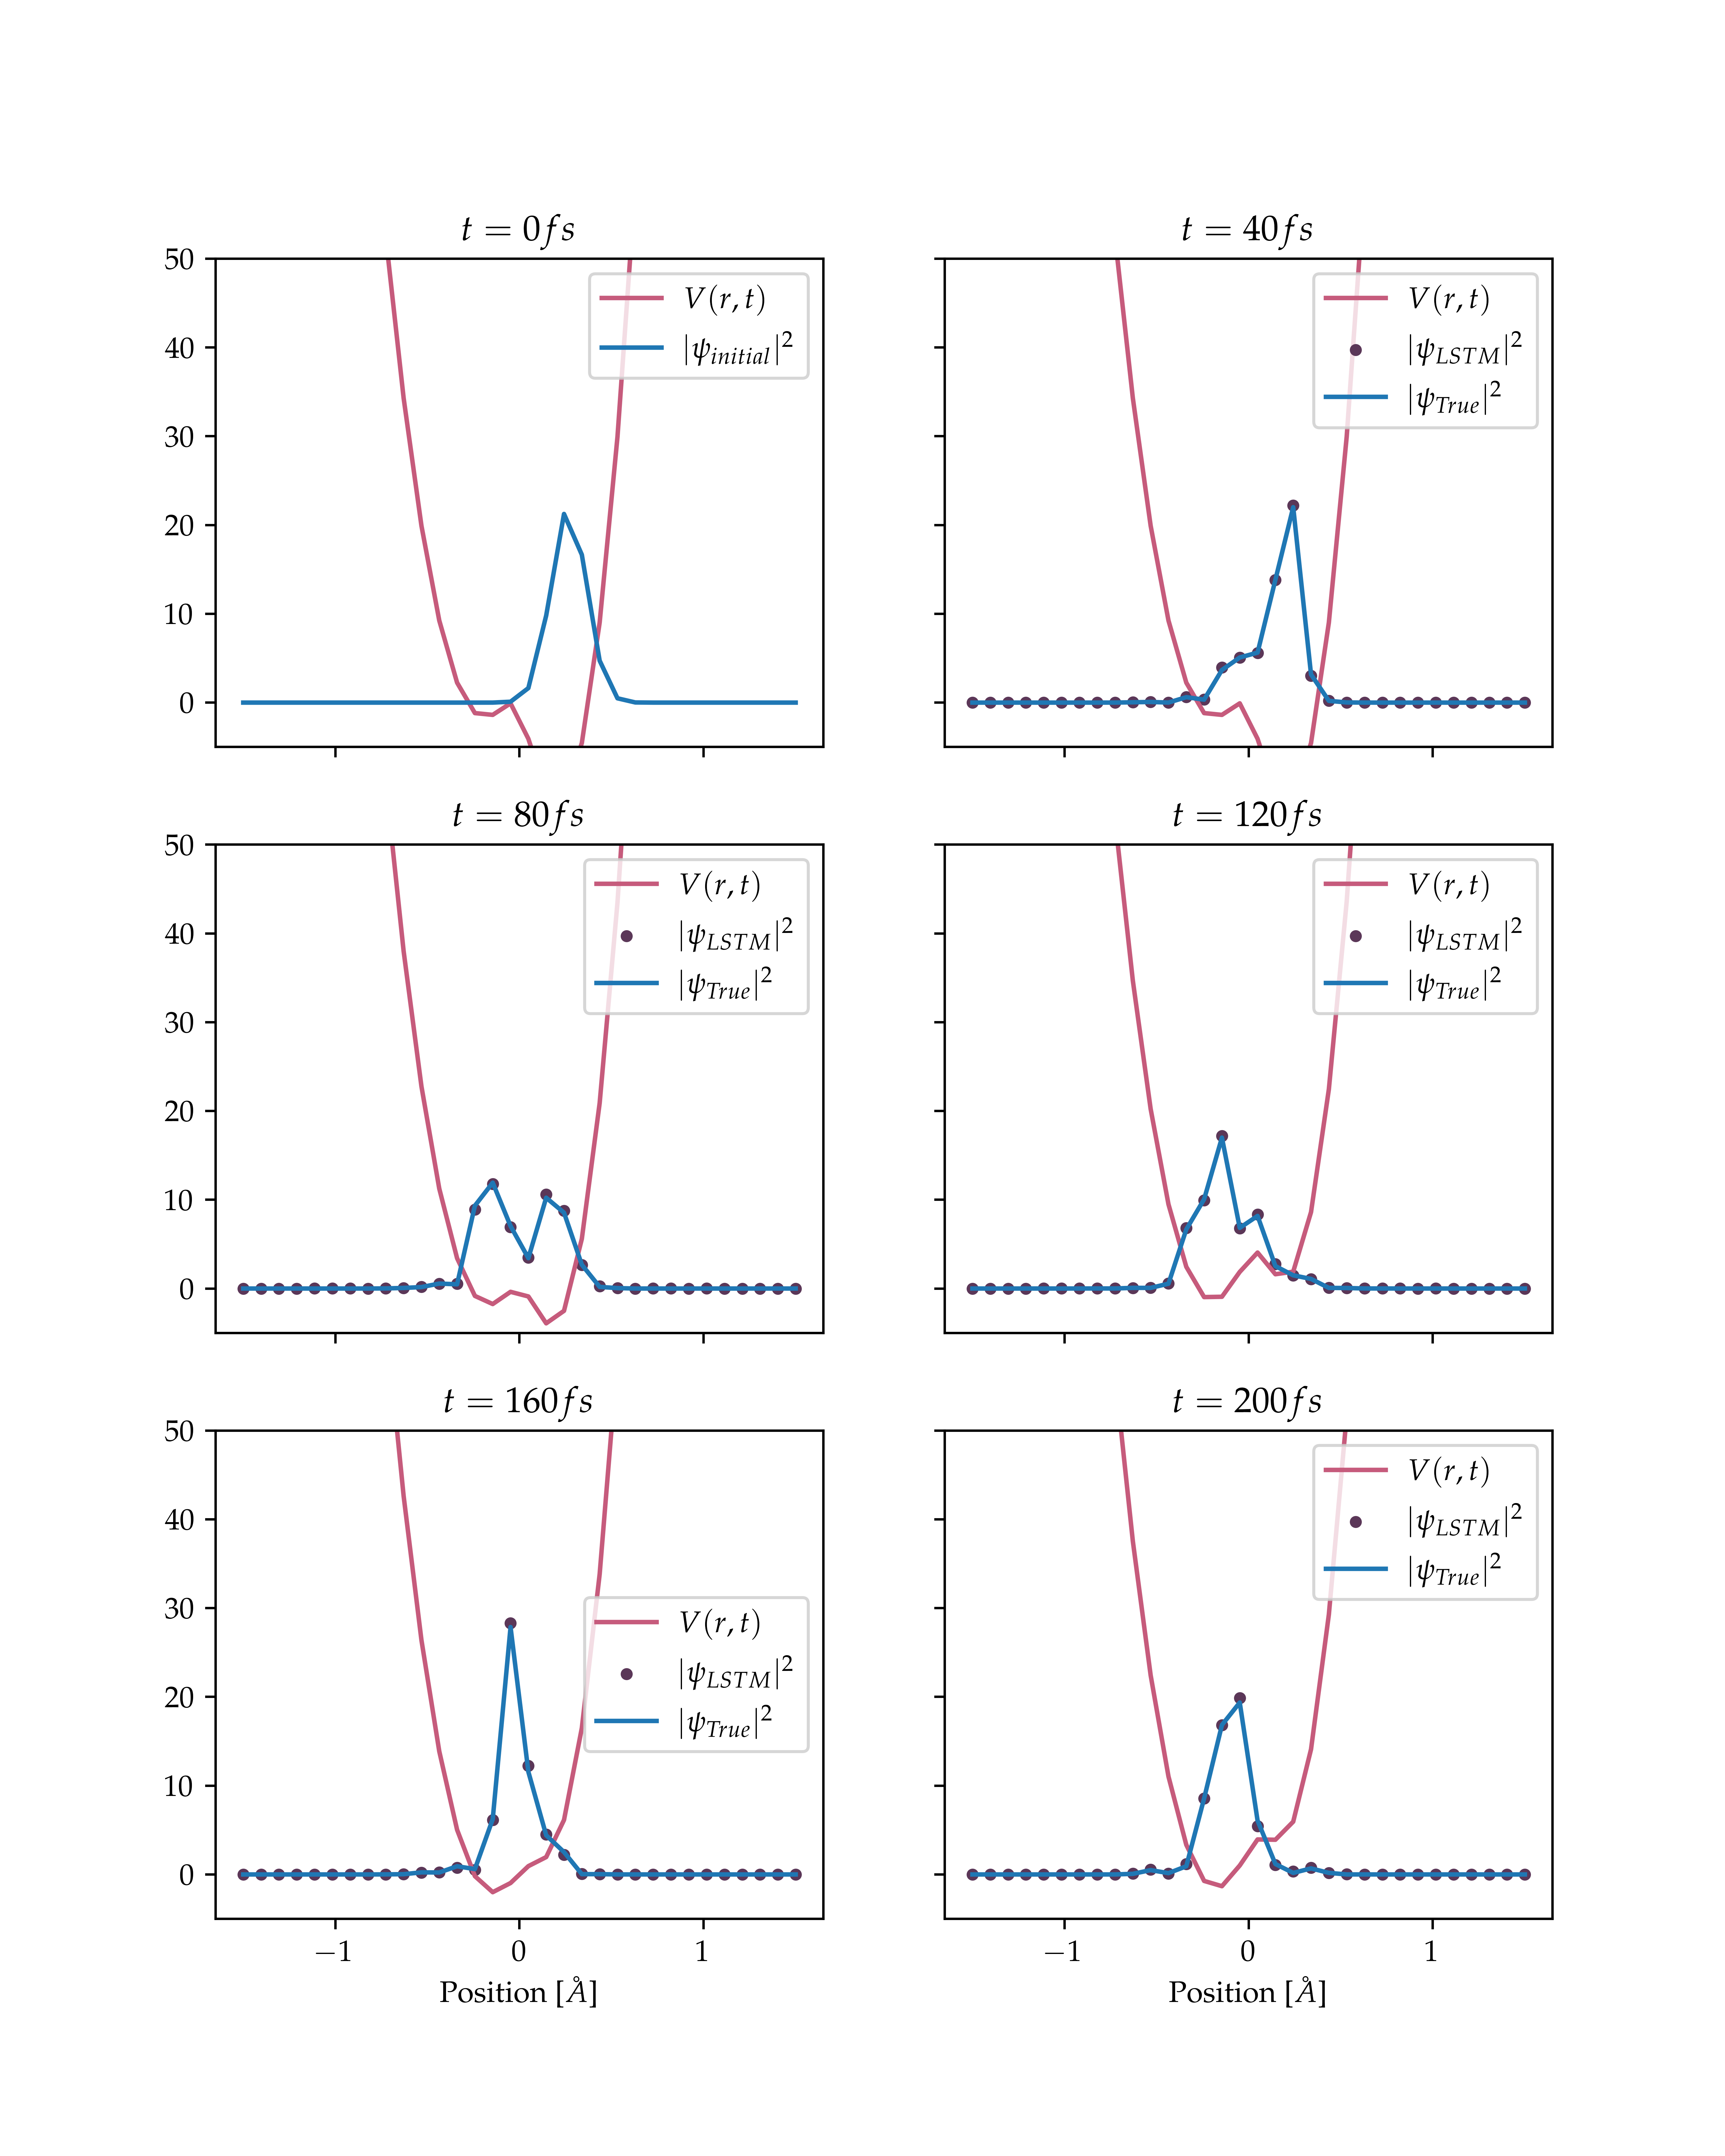
\includegraphics[width=1.4\textwidth]{./img/model/trajDens7.png}}
  \caption{Ejemplo 1 de predicción para una trayectoria completa de $200\,fs$.\\ Las densidades de probabilidad $|\psi|$ están escaladas para poder visualizar el potencial en la misma gráfica.}
  \label{fig:trajec1}
\end{figure}

\begin{figure}[H]
  \centering
  \makebox[\textwidth][c]{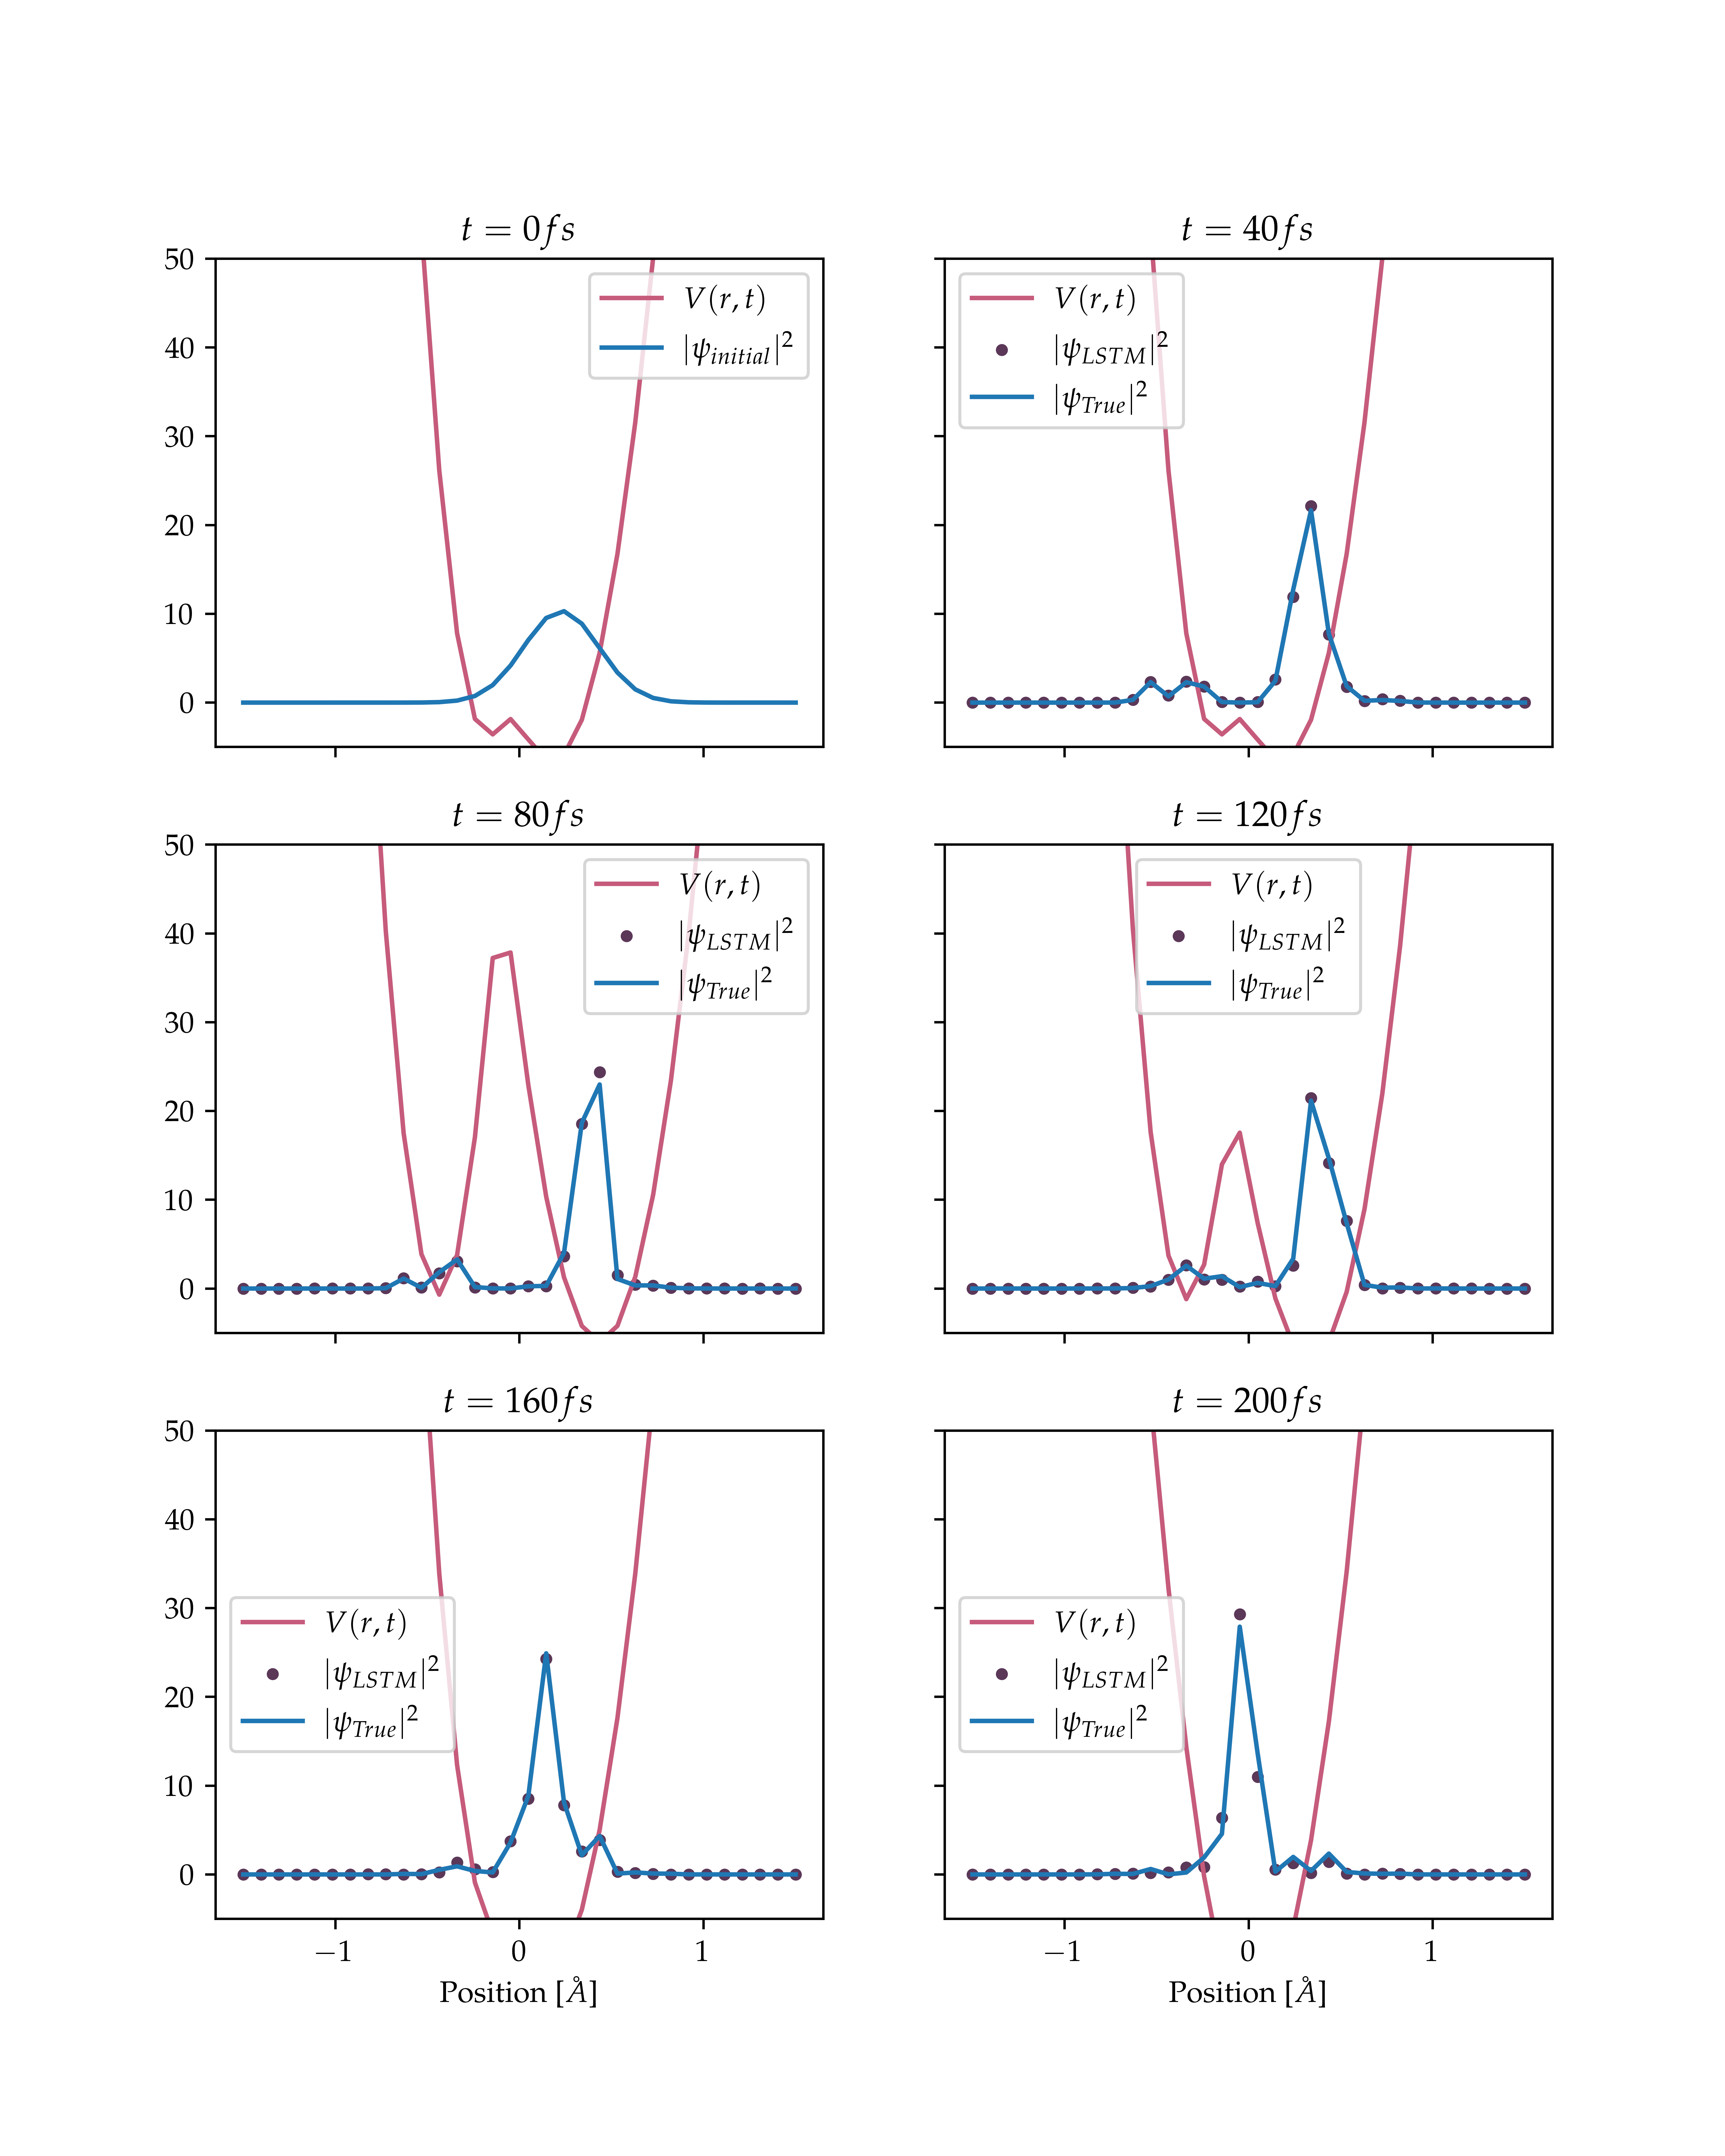
\includegraphics[width=1.4\textwidth]{./img/model/trajDens1.png}}
  \caption{Ejemplo 2 de predicción para una trayectoria completa de $200\,fs$.\\ Las densidades de probabilidad $|\psi|$ están escaladas para poder visualizar el potencial en la misma gráfica}
  \label{fig:trajec2}
\end{figure}

\begin{figure}[H]
  \centering
  \makebox[\textwidth][c]{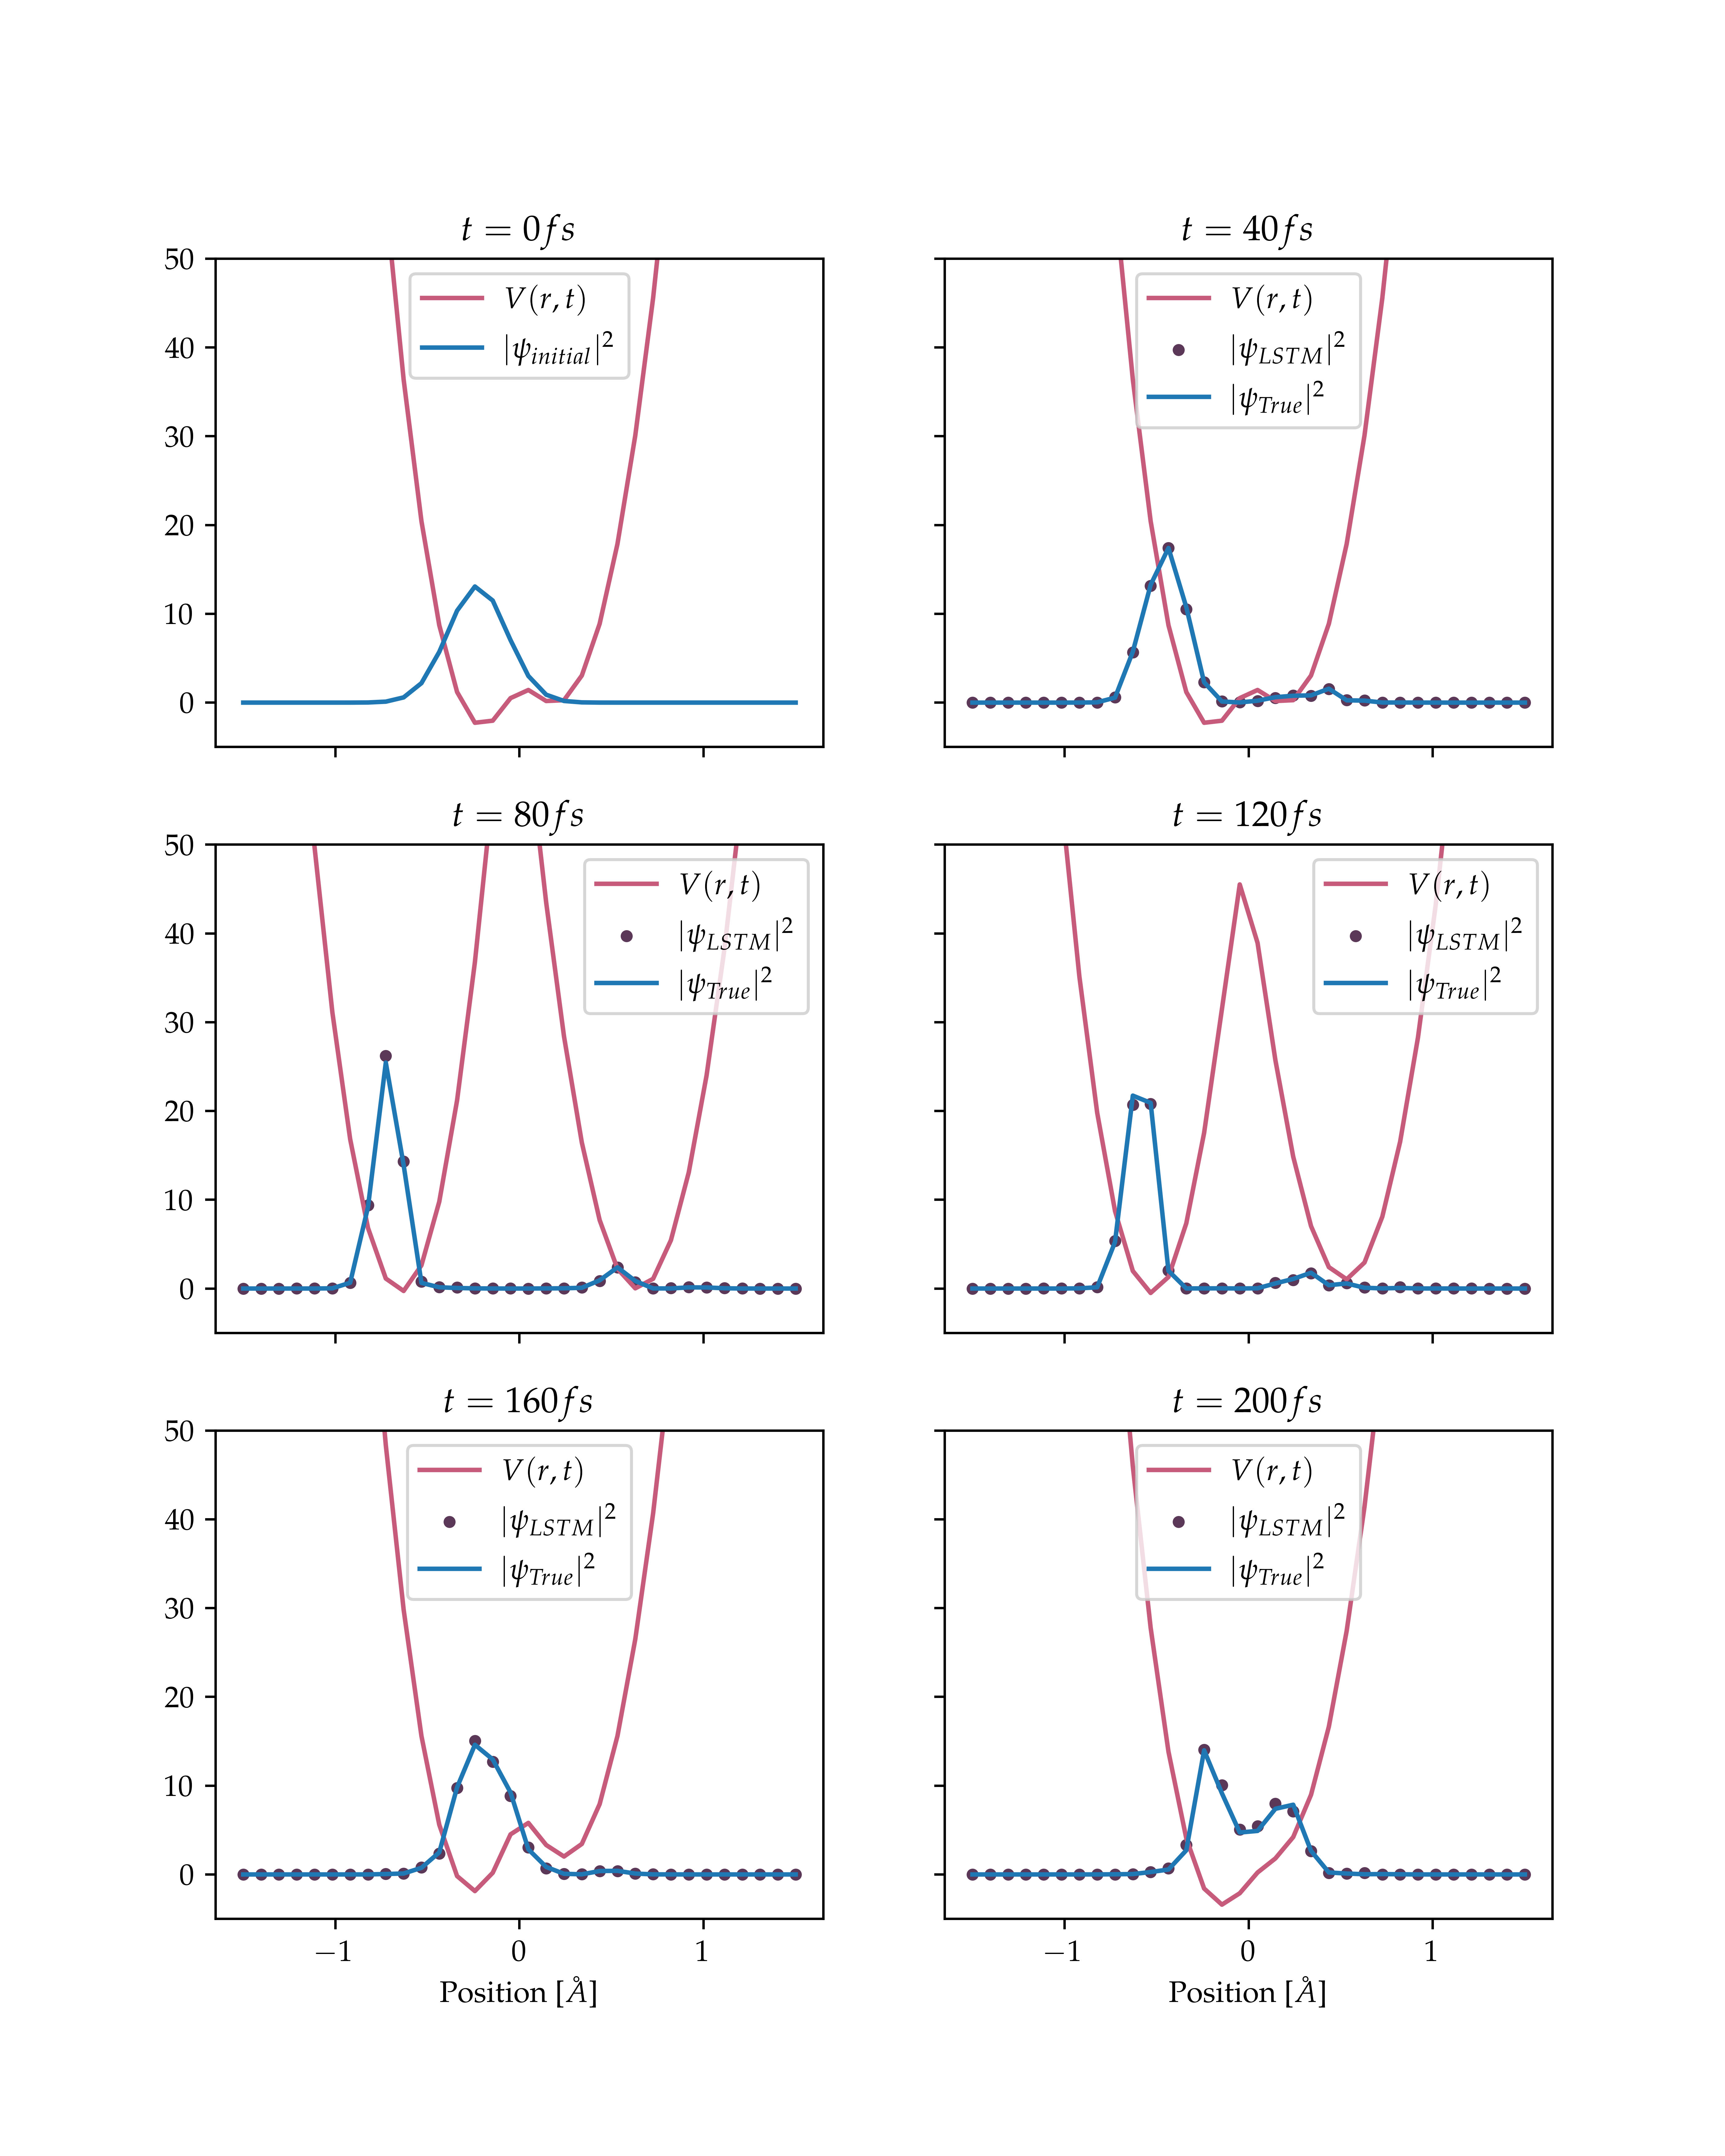
\includegraphics[width=1.4\textwidth]{./img/model/trajDens5.png}}
  \caption{Ejemplo 3 de predicción para una trayectoria completa de $200\,fs$.\\ Las densidades de probabilidad $|\psi|$ están escaladas para poder visualizar el potencial en la misma gráfica}
  \label{fig:trajec3}
\end{figure}

En las gráficas anteriores se observa que la red es capaz de predecir la evolución temporal de una onda inicial hasta $200\,fs$ después, dado que la escala de tiempo característico del movimiento vibratorio de protones es de $10\,fs$ a $25\,fs$ \cite{Main:2021}, la red puede predecir al menos 8 veces más esta escala de tiempo característico.  


\subsection{Aumento de resolución con dos LSTM}

Una manera de aumentar la resolución de la red, es decir, aumentar el número de puntos en la malla es tomar una división de $N=64$ puntos en la malla para la onda inicial $\psi(r,t=0)$ y los potenciales $V(r,t)$, y dividirlos en dos grupos de $N_{azul}=32$ y $N_{rojo}=32$ de manera distribuida en la malla, como se muestra en la \autoref{fig:aumento}. 

\begin{figure}[H]
  \centering
  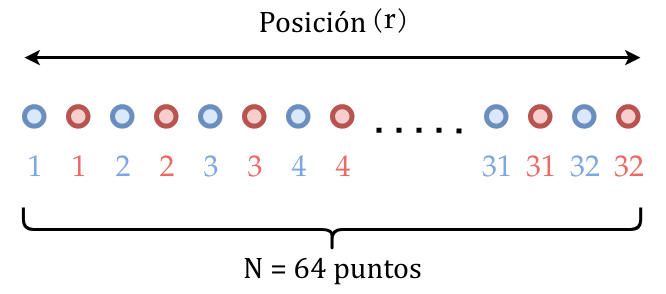
\includegraphics[width=0.5\textwidth]{./img/aumento.drawio.png}
  \caption{División de 64 puntos en el espacio de posiciones en dos grupos.}
  \label{fig:aumento}
\end{figure}

De esta forma, se tienen los valores correspondientes: $\psi_{azul}(r,t=0)$, $V_{azul}(r,t)$, $\psi_{rojo}(r,t=0)$ y $V_{rojo}(r,t)$, en donde cada uno tiene entradas de $N=32$ puntos, que se ajustan al tamaño de la entrada de la red. Así, utilizando dos veces la misma red, una vez para cada grupo de puntos, se obtienen los resultados a cada tiempo $t$ para un malla de tamaño de $N=64$ puntos.
\\
Las siguientes gráficas muestran el resultado de aplicar este método.

\begin{figure}[H]
  \centering
  \makebox[\textwidth][c]{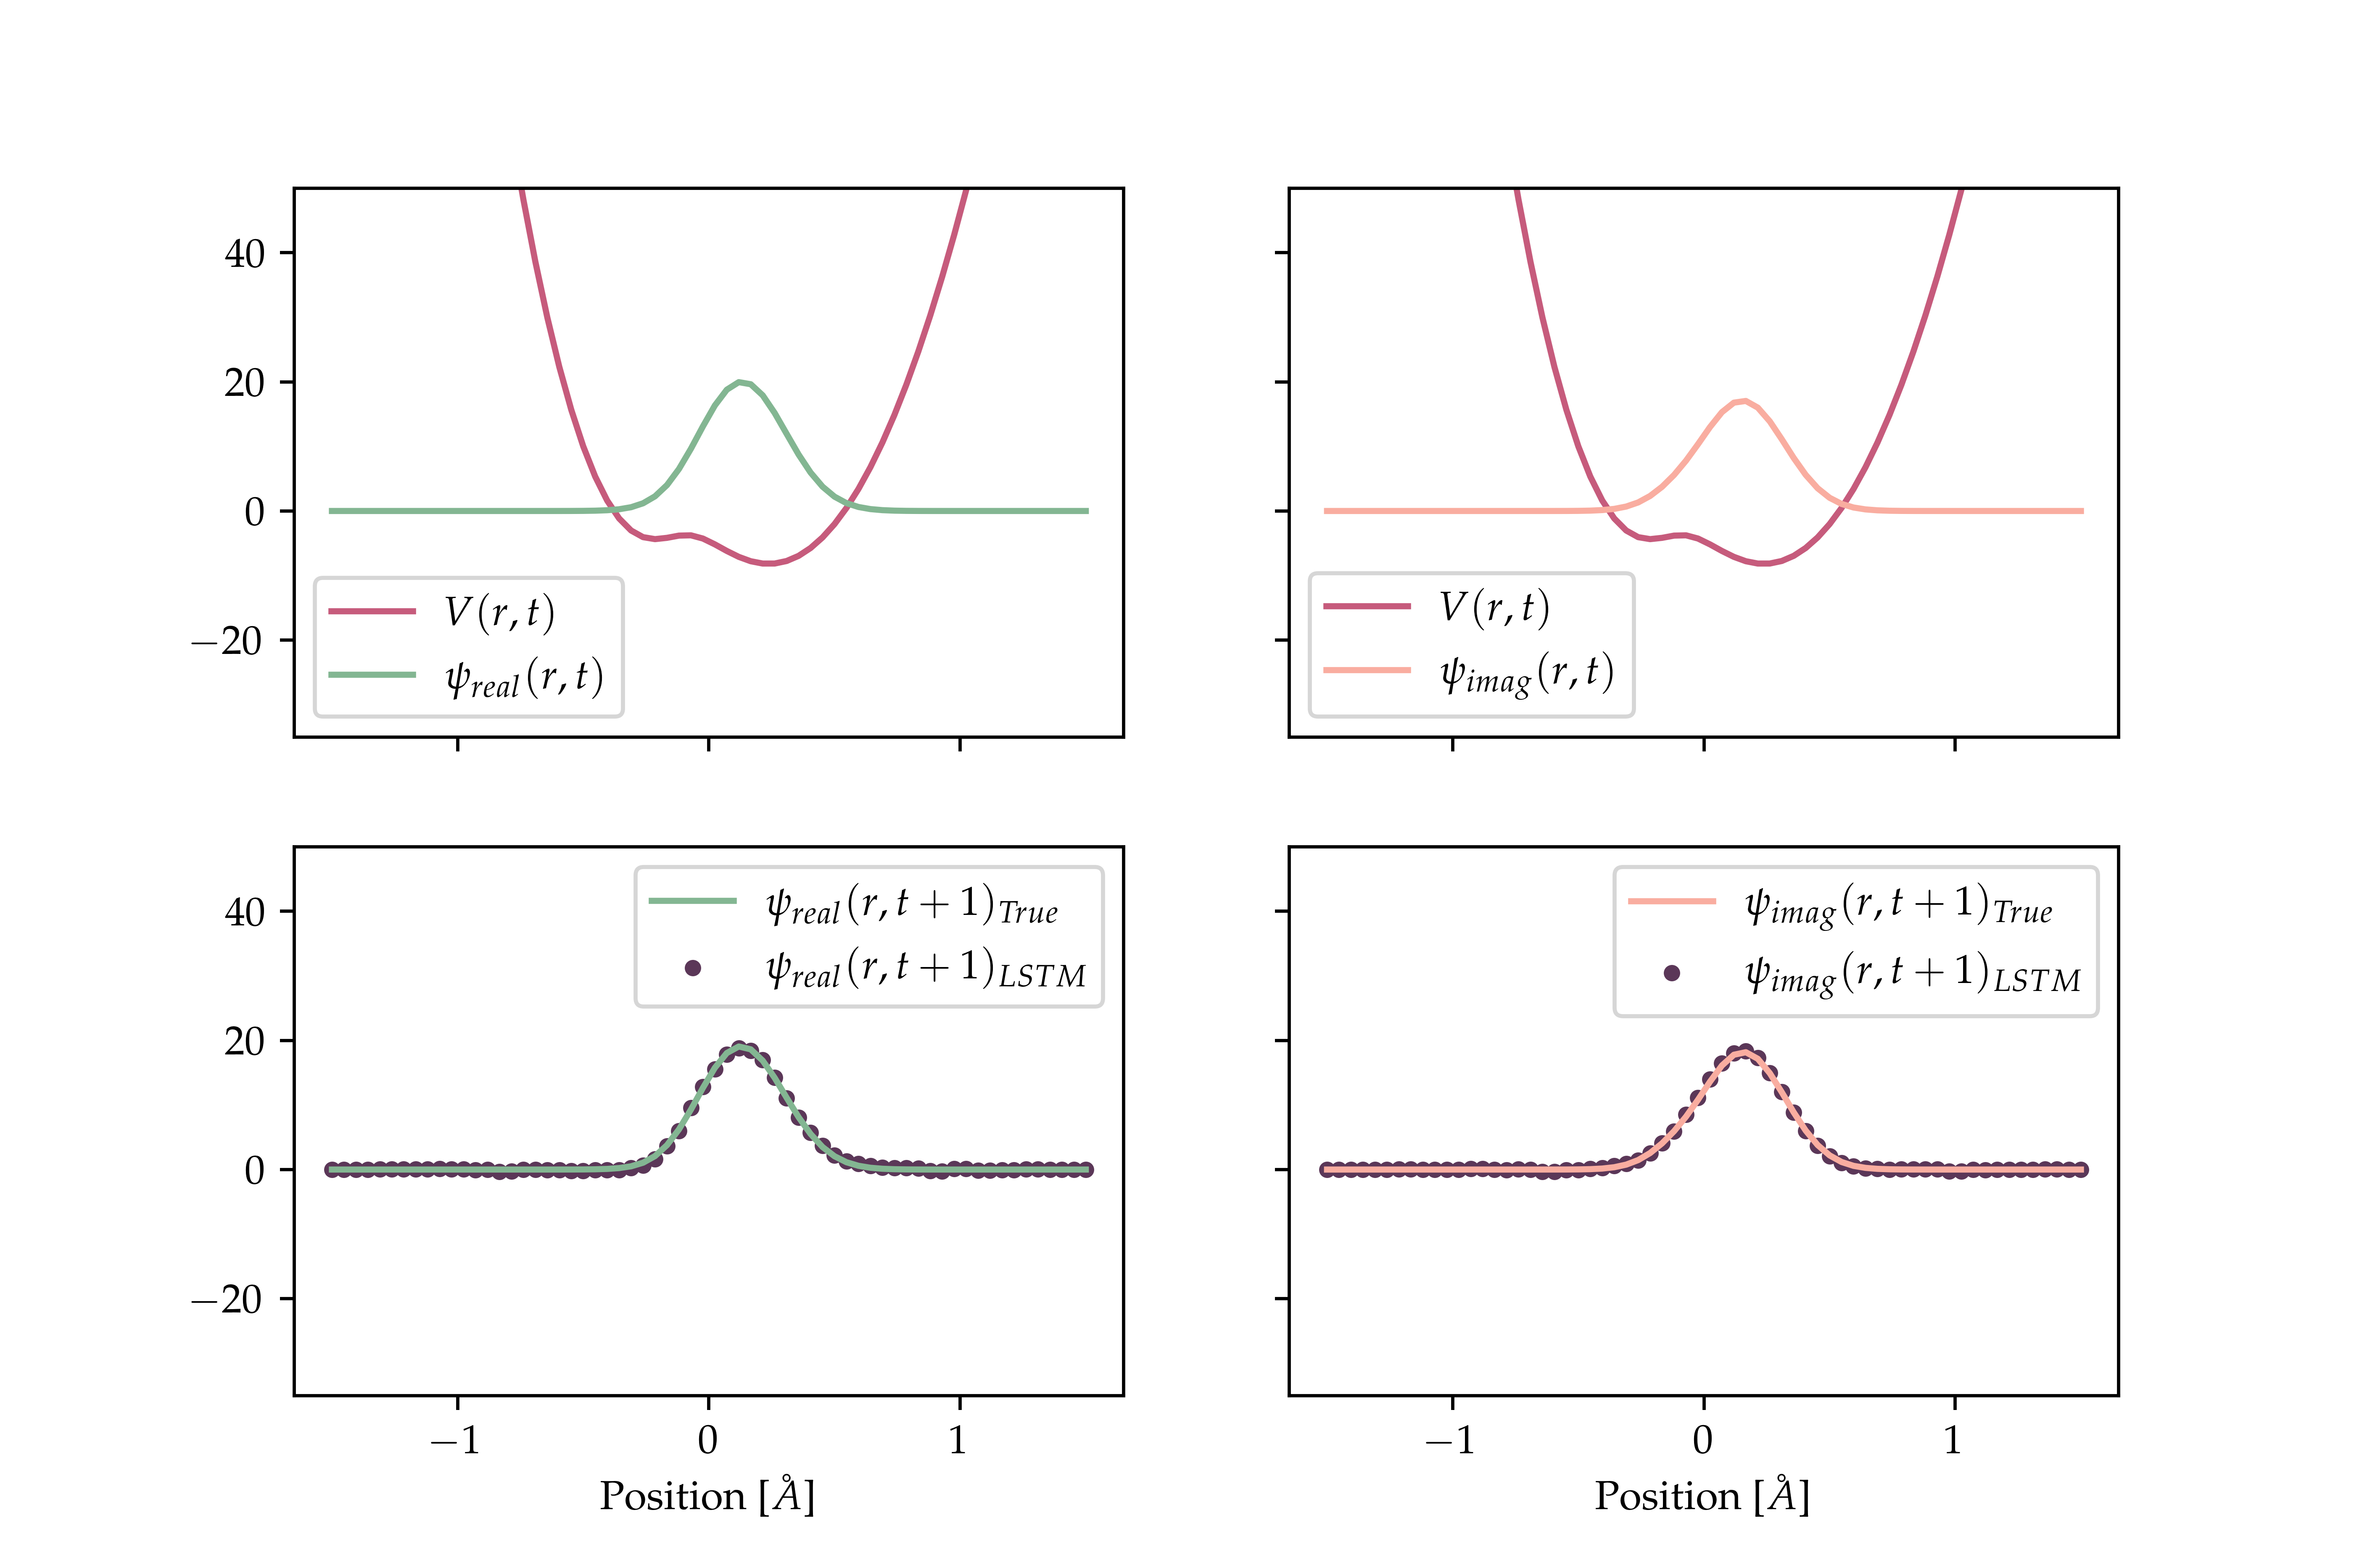
\includegraphics[width=1.1\textwidth]{./img/model/1step64size.png}}
  \caption{Ejemplo 1 de predicción a un paso de tiempo $\Delta t = 1\,fs$, $N=64$ puntos.\\ Las funciones de onda $\psi$ están escaladas para poder visualizar el potencial en la misma gráfica.}
  \label{fig:1step164}
\end{figure}

\begin{figure}[H]
  \centering
  \makebox[\textwidth][c]{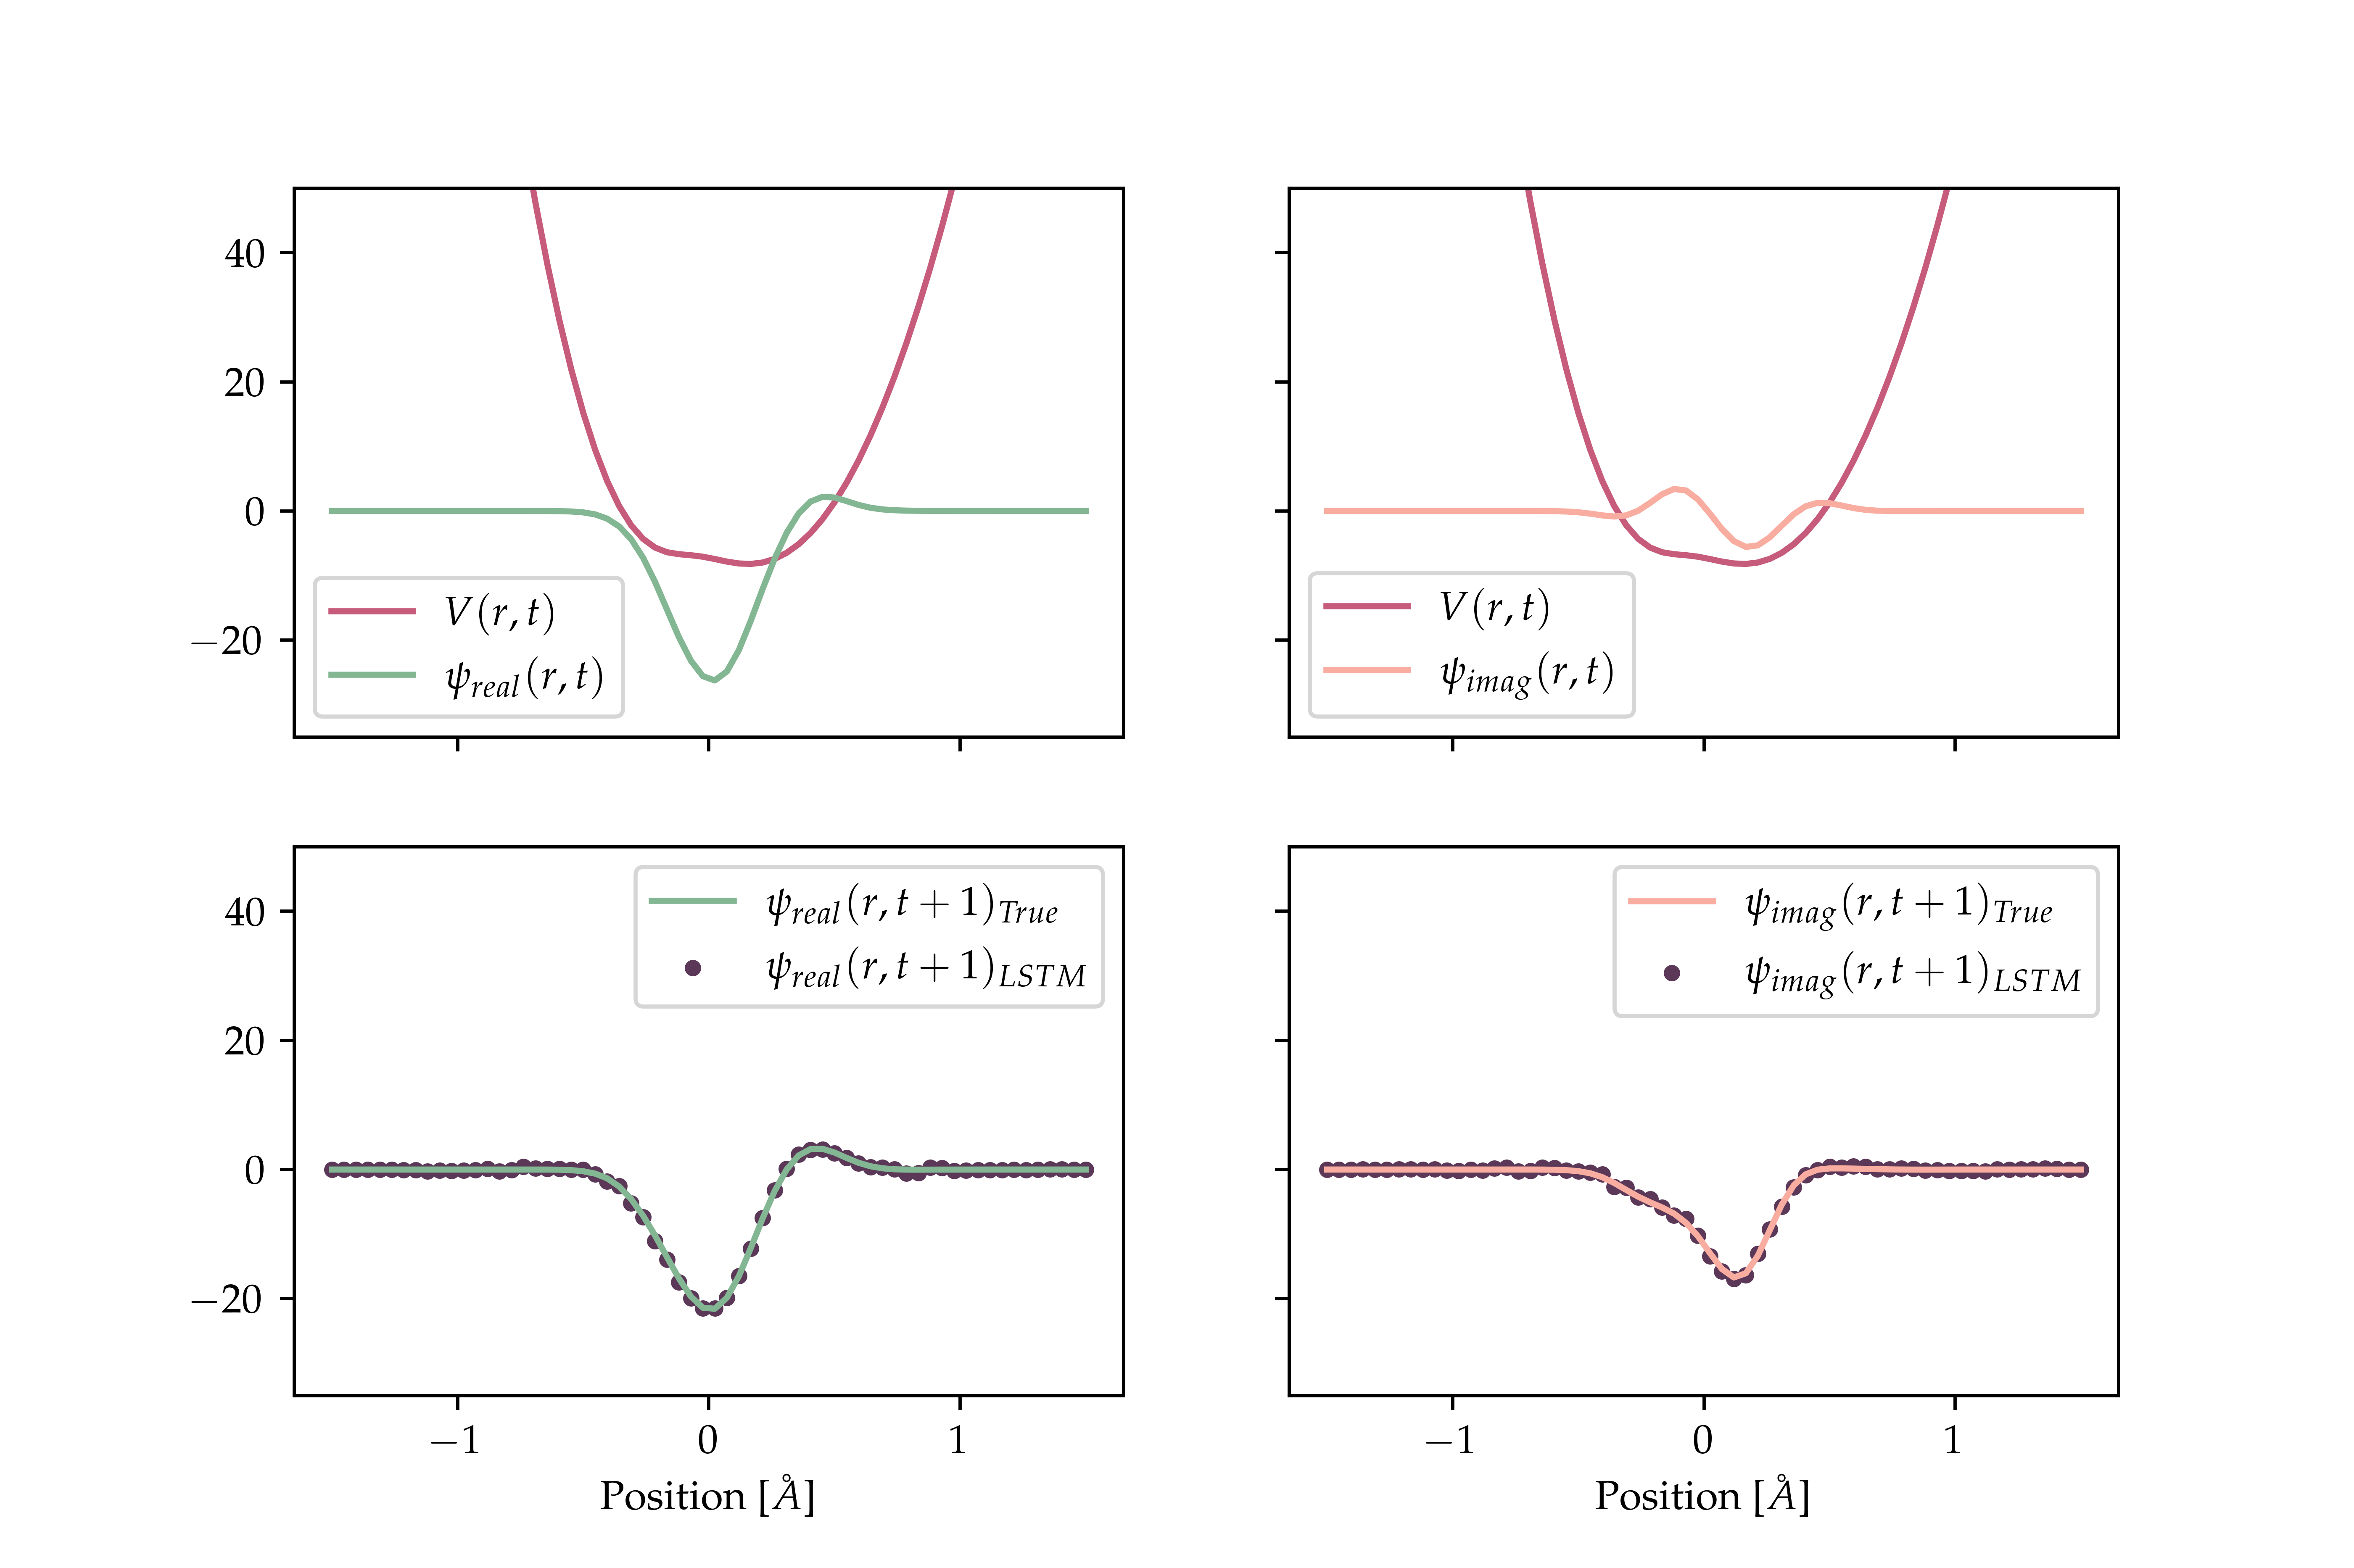
\includegraphics[width=1\textwidth]{./img/model/1step64size1.png}}
  \caption{Ejemplo 2 de predicción a un paso de tiempo $\Delta t = 1\,fs$, $N=64$ puntos.\\ Las funciones de onda $\psi$ están escaladas para poder visualizar el potencial en la misma gráfica.}
  \label{fig:1step264}
\end{figure}

\begin{figure}[H]
  \centering
  \makebox[\textwidth][c]{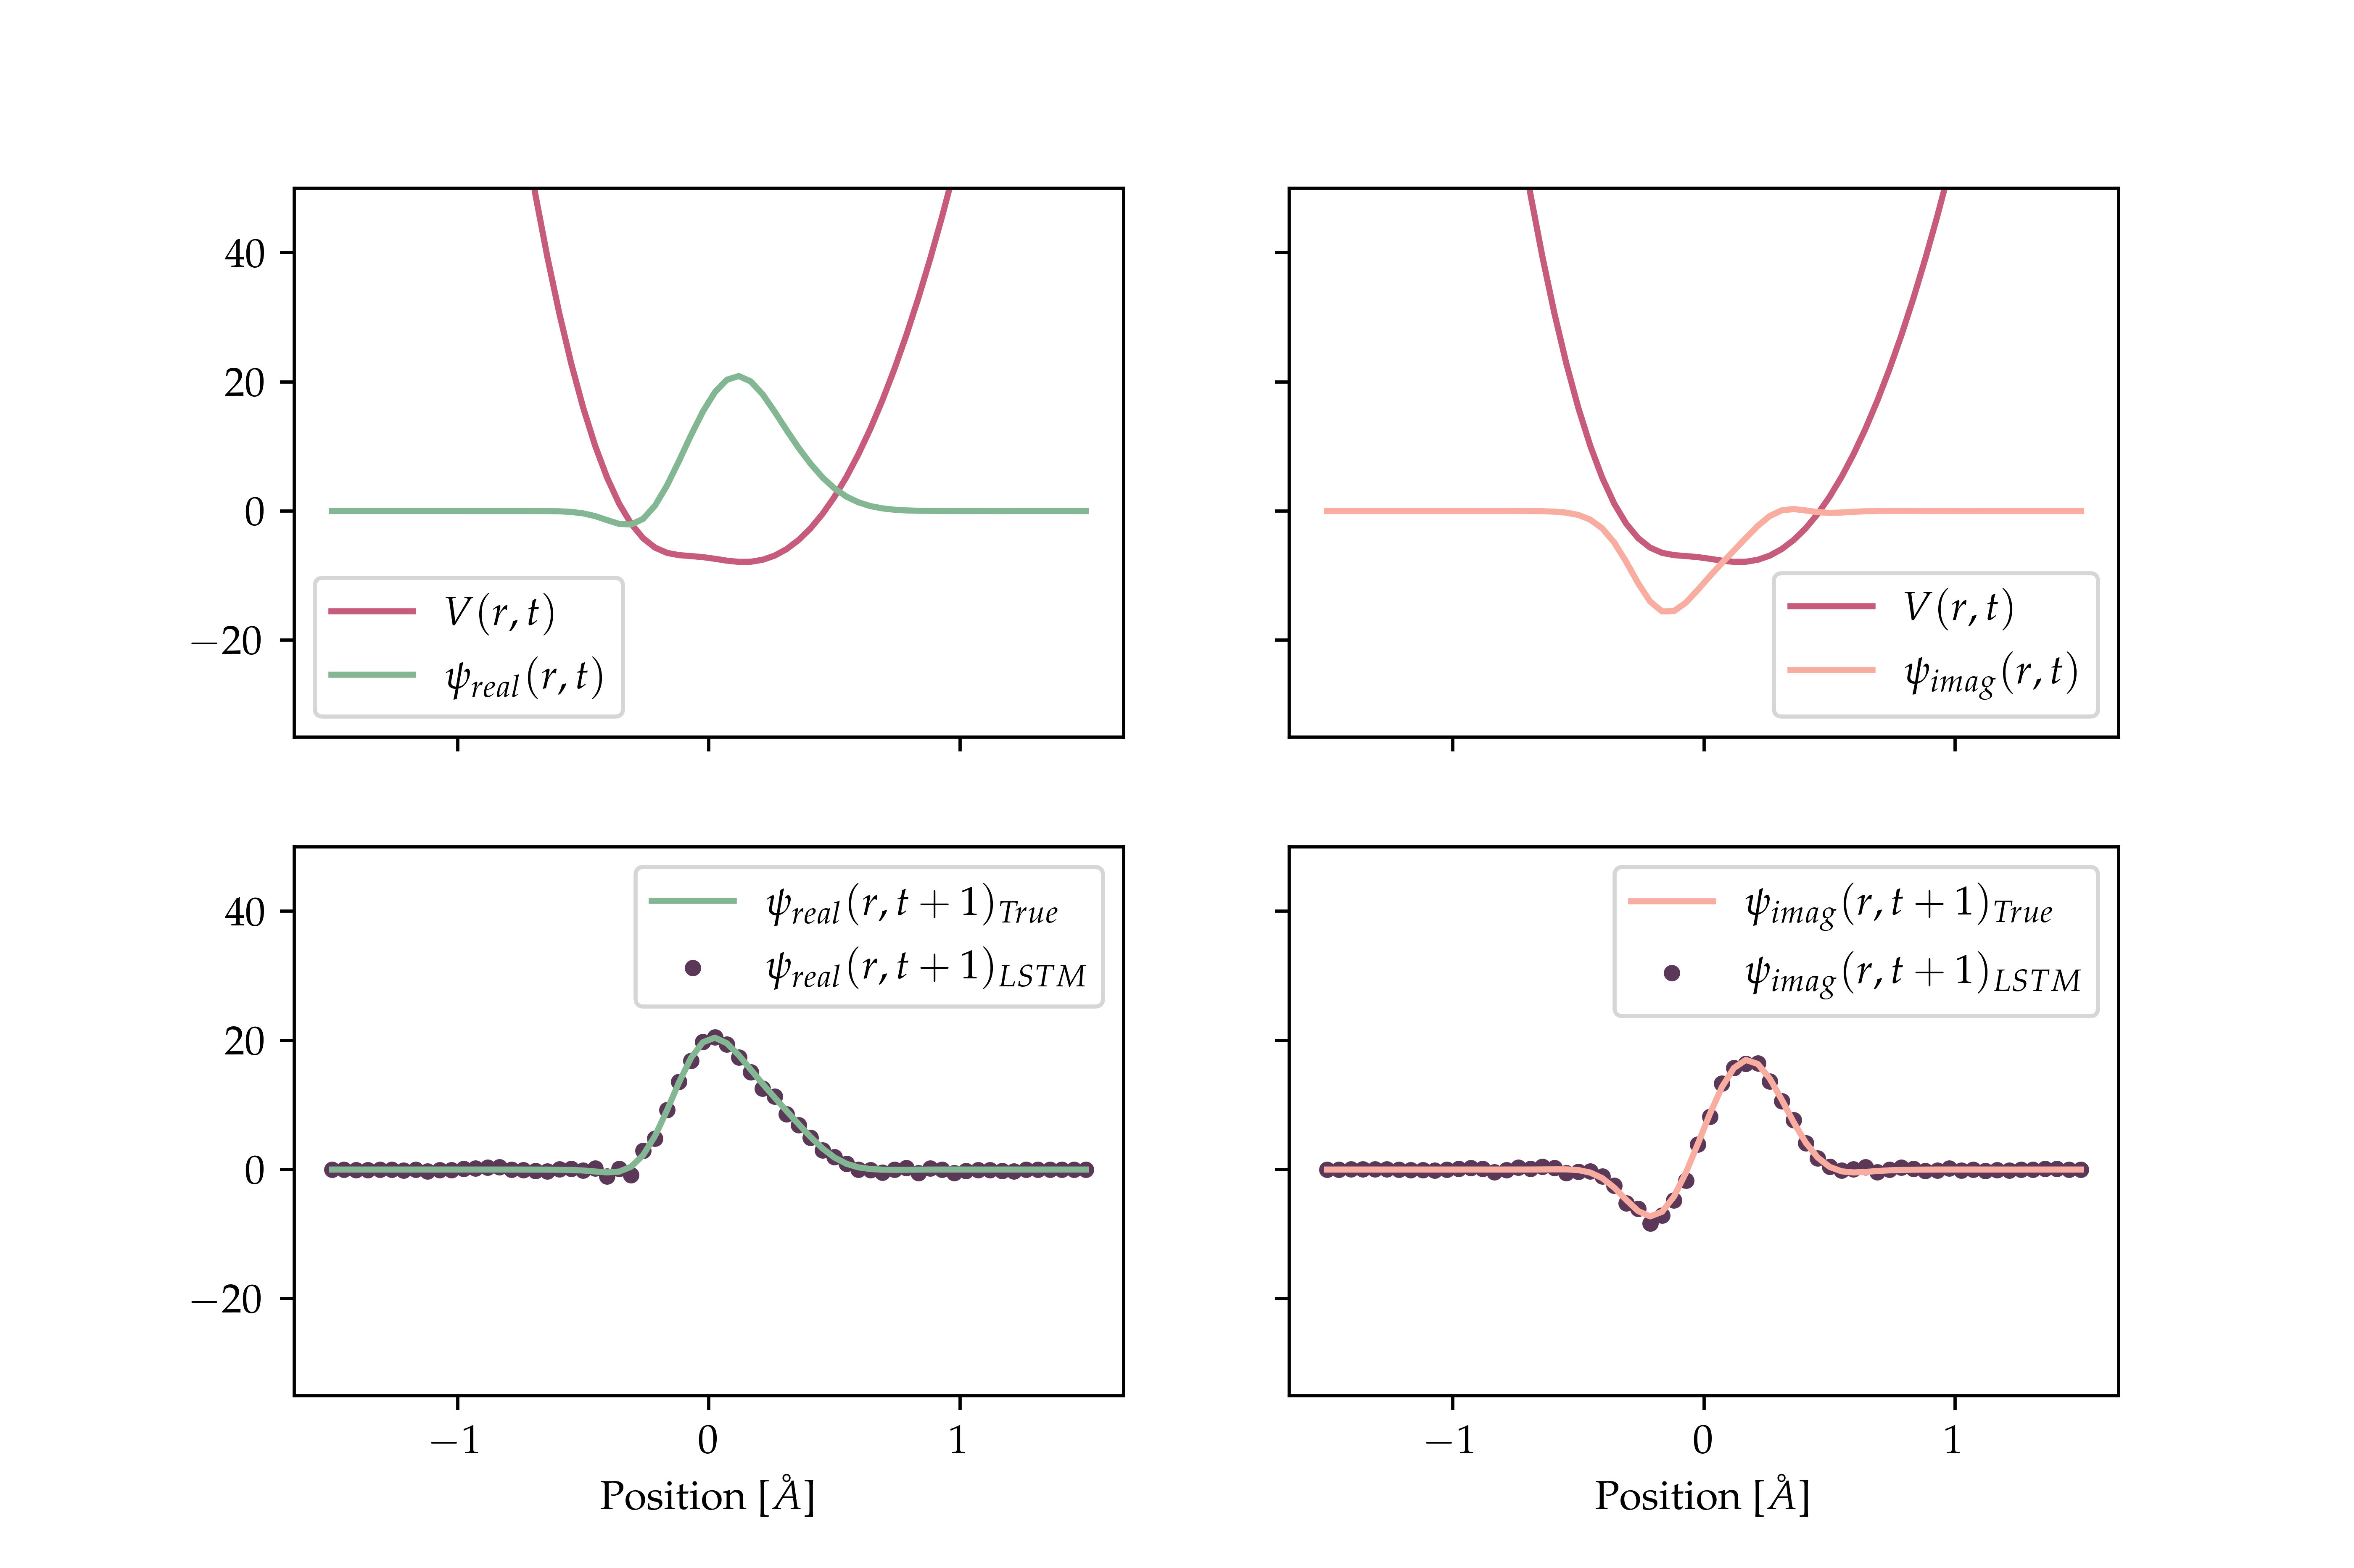
\includegraphics[width=1\textwidth]{./img/model/1step64size2.png}}
  \caption{Ejemplo 3 de predicción a un paso de tiempo $\Delta t = 1\,fs$, $N=64$ puntos.\\ Las funciones de onda $\psi$ están escaladas para poder visualizar el potencial en la misma gráfica.}
  \label{fig:1step364}
\end{figure}

La siguiente gráfica muestra la evolución temporal de la densidad de probabilidad $|\psi(r,t)|$ bajo un potencial $V(r,t)$ aplicando el método de aumento de resolución de puntos.

\begin{figure}[H]
  \centering
  \makebox[\textwidth][c]{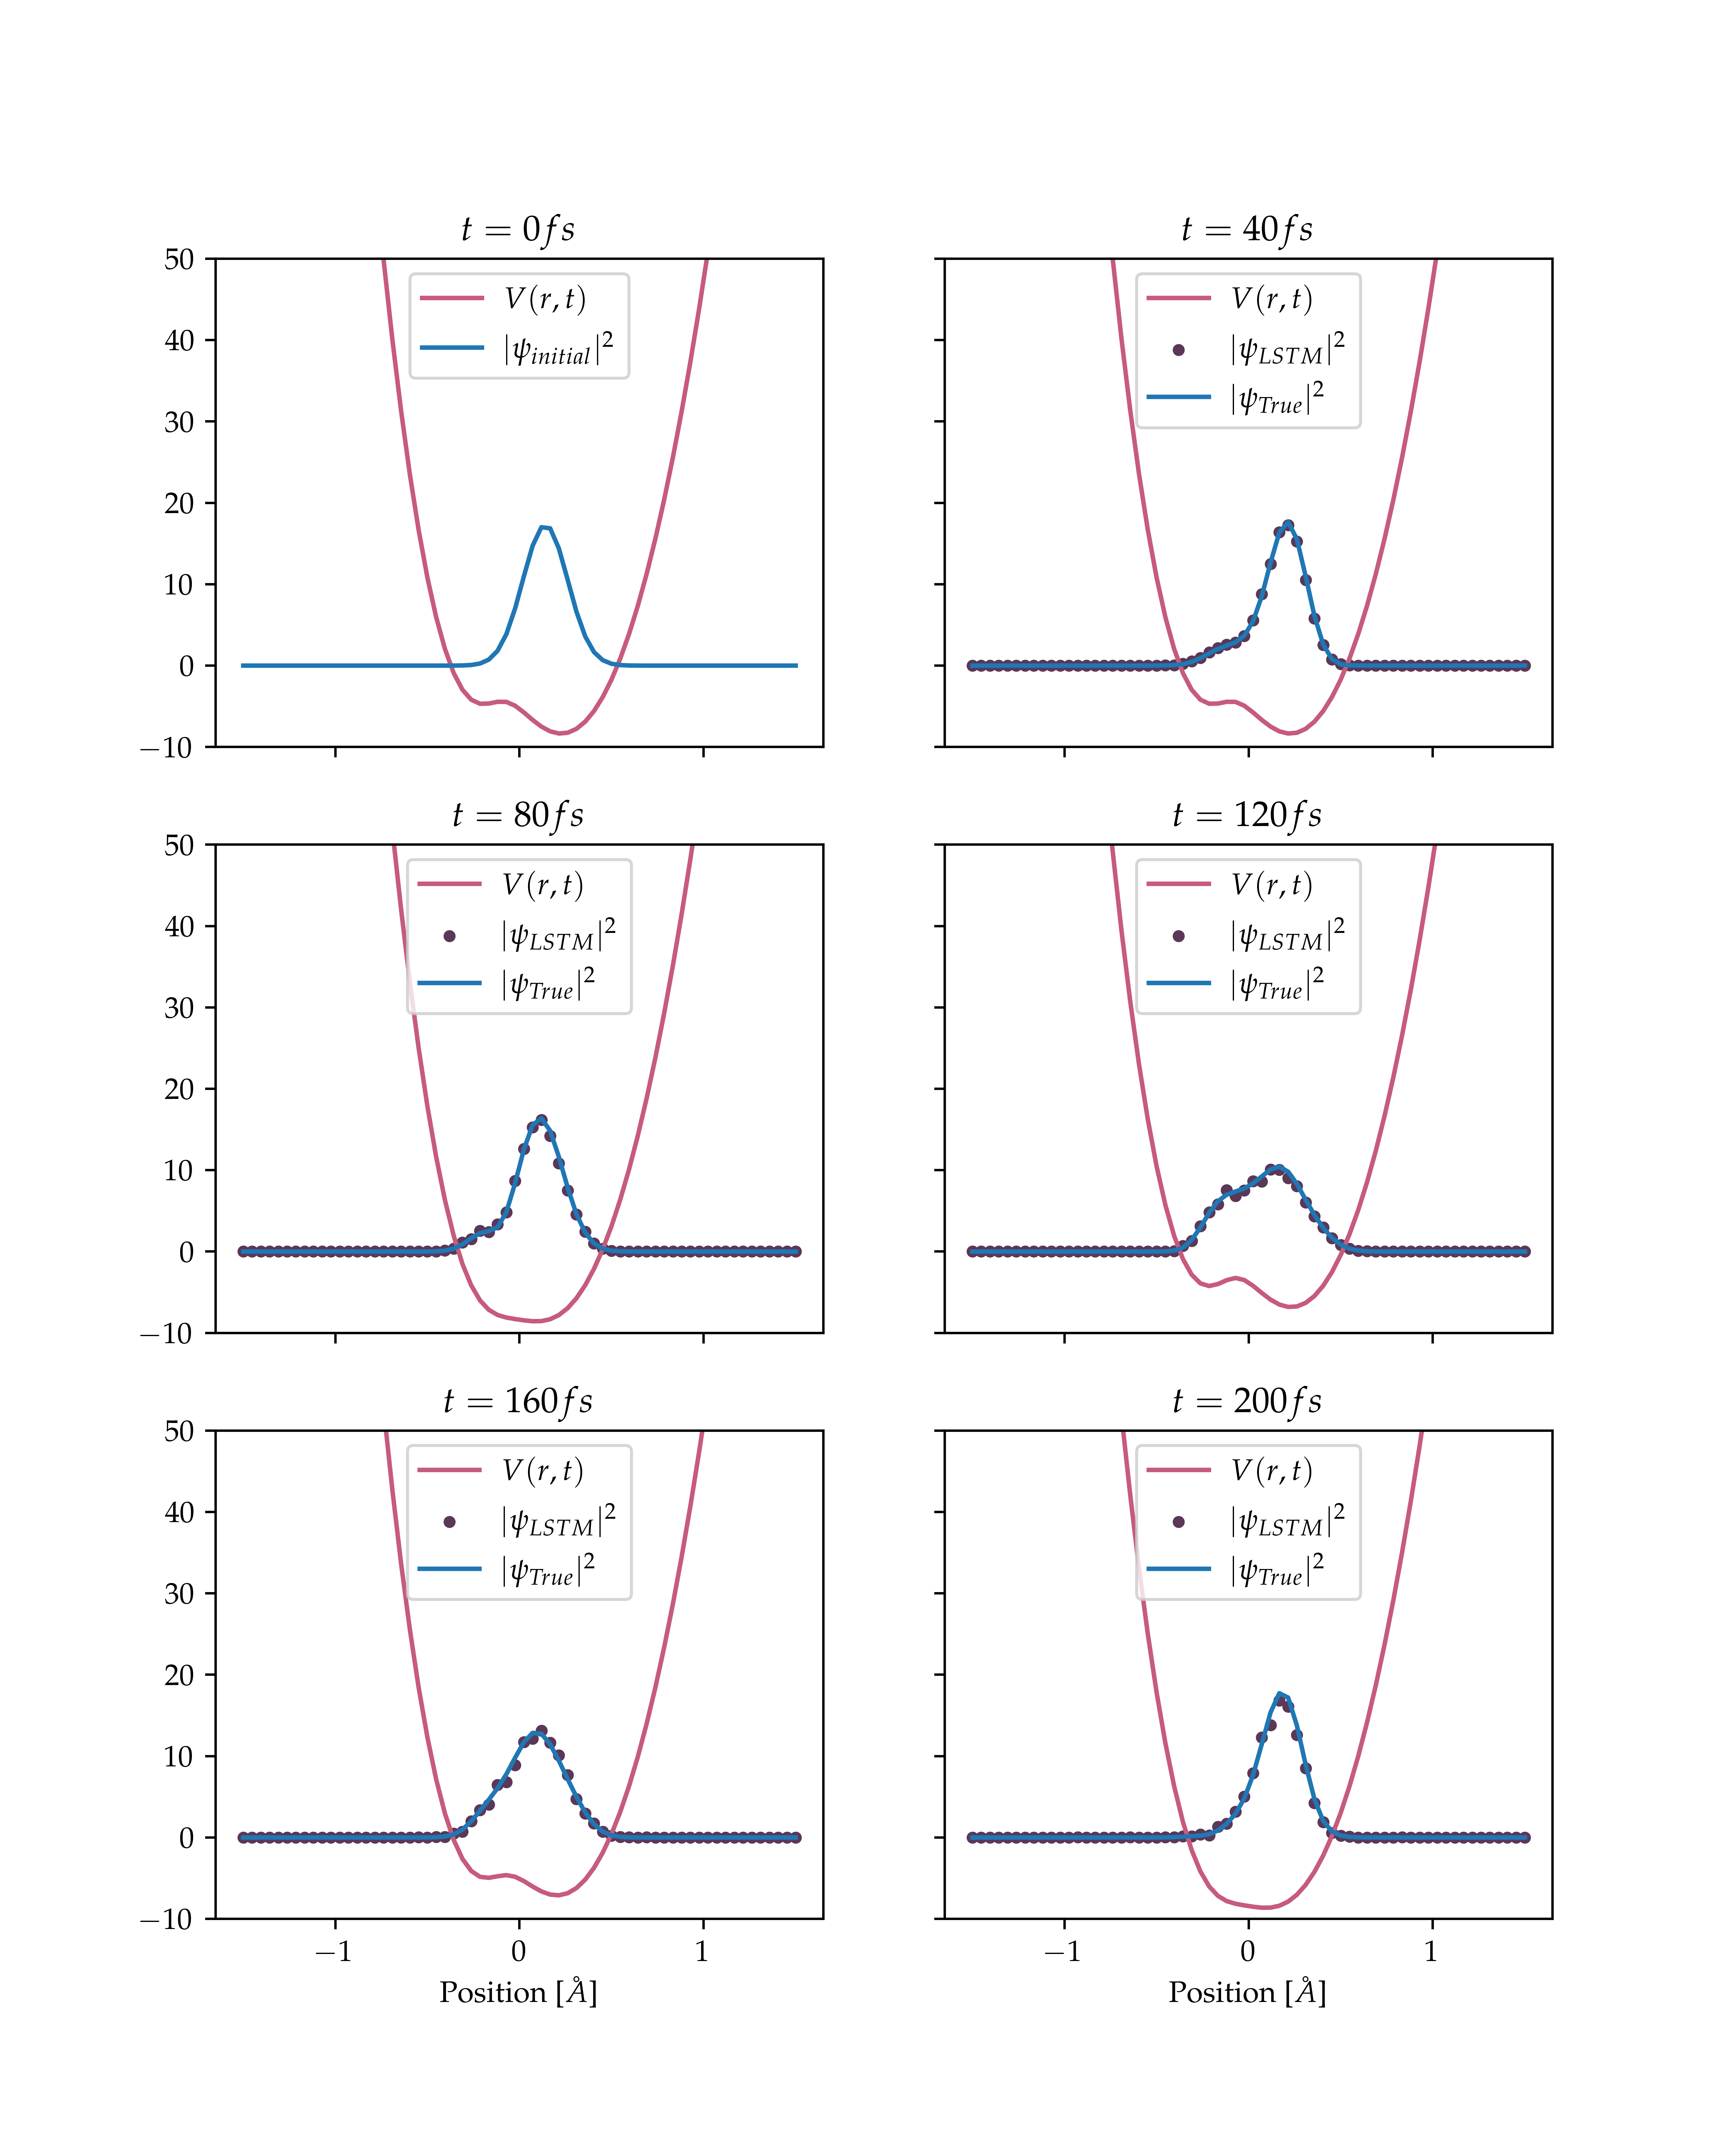
\includegraphics[width=1.4\textwidth]{./img/model/trajDens64size.png}}
  \caption{Ejemplo de predicción para una trayectoria completa de $200\,fs$, $N=64$ puntos.\\ Las densidades de probabilidad $|\psi|$ están escaladas para poder visualizar el potencial en la misma gráfica}
  \label{fig:trajec1_64}
\end{figure}

\subsection{Conclusión}
La evolución temporal de un sistema cuántico se encuentra resolviendo la ecuación de Schrödinger \autoref{eq:TDSE ket}, cuando el Hamiltoniano del sistema es dependiente del tiempo, encontrar el operador de propagación, que es una solución general de la ecuación, puede ser un proceso complicado para los métodos analíticos, o costoso en tiempo computacional para los métodos numéricos. En este trabajo se desarrolló una alternativa para resolver la \acs{TDSE} utilizando una red neuronal artificial tipo long short-term memory como propagador, encontrando que la red entrenada necesita menos tiempo de ejecución para propagar una onda en comparación a otros métodos numéricos, con una calidad de predicción promedio de $0.946$ para la magnitud $|S|$ y $0.0001$ para la fase absoluta $\theta$. \\
Como propuesta para trabajos futuros se presentan las siguientes sugerencias:
\begin{itemize}[label=\textcolor{CTtitle}{\textbullet}]
\item Utilizar más puntos en la malla: Generar datos con más puntos en la malla requieren de un mayor tiempo de computación, sin embargo la calidad en las predicciones puede mejorar significativamente, esperando resultados como los que se presentan en la sección \autoref{sec:ProtonTransfer}.
\item Implementar el modelo para dos dimensiones en el espacio de posiciones: En el documento de información adicional de la referencia \cite{Main:2021} se proporcionan las ecuaciones para modelar el potencial en dos dimensiones.
\end{itemize}